%%% PART B 
%  \macror Keywords and input data formatting 
%% \macror = cmbx10 scaled\magstep2
%\macror Glossary of keywords 
%\part{Keywords and input data formatting}{Keywords and input data formatting}

%%   ZGlossaire 2

\section*{INTRODUCTION}
\addcontentsline{toc}{section}{\numberline{}INTRODUCTION}

Here after is given a detailed description of input data formatting 
and units. All available keywords appear in alphabetical order.  
\bigskip

\noindent Keywords are read from the input data file by an unformatted 
\textsl{FORTRAN READ} statement. They  be enclosed between quotes (\emph{e.g.}, `\textsl{DIPOLE}').  
\bigskip

\noindent Text string data such as comments or file names, are read by 
formatted READ statements, no quotes should be used in that case. 

\bigskip

Numerical variables 
and indices are read by unformatted READ. It may therefore be necessary that 
integer variables be assigned an integer value.  
\bigskip

\noindent In the following tables 
\begin{itemize}
	\item[$\bullet$] the first column shows the expected input parameters (actually, their \textsl{values} are expected), 
indices and text strings,
	\item[$\bullet$]  the second column gives brief comments regarding their meaning and use,
	\item[$\bullet$]  the third column gives the units or ranges, 
	\item[$\bullet$] the fourth column indicates whether the expected  parameter types are 
integer (I), real (E) or text string (A). For example, ``I, 3*E''
 means that one integer followed by 3 reals is expected. 
``A80'' means that a text string of maximum 80 characters is expected. 
\end{itemize}

\clearemptydoublepage

%%%%%%%%%%%%%%%%%%%%%%%%%%%%%%%%%%%%%%%%%%%%%%%%%%%%%%%%%%%%%%%%%%%%%%%%%%%%%%%%%%%%%%%%
\newcommand{\mestab}{
~ ~ $ \omega^+$, $\theta$,     $R_1$, $U_1$, $U_2$, $R_2 $     \quad \=
 �$ B=\mathcal{F}B_0 \left(1+N \left(\frac{R-RM }{ RM} \right)      
                +B \left(\frac{R-RM}{ RM} \right)^2+G \left(\frac{R-RM }{ RM}
                \right) \right) $, more    \quad \= 2*cm, 2*deg, cm ~ ~  \= \kill
}
\newcommand{\mestabOBJ}{$PY$, $PT$, $PZ$, $PP$, $PD$ ~ ~  \quad \= 
        total number of particles~; number of distinct momenta~; more... \quad \=
            IY*IT*IZ*IP*IT*IZ*IP*   \quad \= \kill}
%%%%%%%%%%%%%%%%%%%%%%%%%%%%%%%%%%%%%%%%%%%%%%%%%%%%%%%%%%%%%%%%%%%%%%%%%%%%%%%%%%%%%%%%


\begin{tabbing}
\mestab
\textbf{AGSMM}         \label{AGSMM-B} \index{AGSMM|textbf}
           \>\textbf{\AGSMMTitl}\> \>\\
\\
\\
 $\IL$   \>$\IL=1,2[\times 10^n],~7$ : print coordinates, fields, etc., along trajectories \>0-2$[\times 10^n]$, 7 \>I\\
         \> in zgoubi.res ($1$),  zgoubi.plt ($2$),  zgoubi.impdev.out ($7$).       \>                   \> \\
 \\
\textsl{MOD[.MOD2]},  $dL$,   \> Type of magnet model~\footnotemark[1]~[type of back-leg winding model~\footnotemark[2]]~; \> 2*no dim., cm, \>I[.I], 5*E\\     
$R_0$, $dB1$, $dB2$, $dB3$ \> unused~; pole tip radius, 10~cm if set to zero~; relative  \>  3*no dim. \>\\     
 \>error on dipole, quadrupole, sextupole component. \>\>\\
 \\
 NBLW,    \>Number of back-leg windings~; for each back-leg winding~:   \> $\leq$2, \textsl{\small NBLW}$\times$  \> I, \textsl{NBLW}$\times$ \\     
\textsl{NBLW times~:}  NW, I    \> number of windings, current.   \>(any, Amp.)  \>  (I, E)  \\     
 \\
 \>\textbf{Entrance face} \>\>\\
$ X_E$, $\lambda_E$, $E_2$,  $E_3 $ \>Integration zone~; fringe field extent : \>2*cm, 2*no dim.\> 4*E\\
 \>dipole fringe field extent = $ \lambda_ E $~; \>\>\\
 \>quadrupole fringe field extent = $ \lambda_ E\ast E_2 $~;\>\>\\
 \>sextuppole fringe field extent = $ \lambda_ E\ast E_3 $ \>\>\\
 \>(sharp edge if field extent is zero) \>\>\\
 \\
 \textsl{NCE}, $ C_0-C_5 $            \>same as \textsl{QUADRUPO} 
 					\>0-6, 6*no dim. \>I, 6*E\\
 \\
 \>\textbf{Exit face} \>\>\\
$ X_S$, $\lambda_S$, $S_2$,  $S_3 $ \>Integration zone~; as for entrance
         \>2*cm, 2*no dim. \> 4*E\\
 \\
 \textsl{NCS}, $ C_0-C_5 $           \> \> 0-6, 6*no dim. \>I, 6*E \\
 \\
$ R1$, $R2$, $R3$   \>Skew angles of field components \>3*rad \>10*E \\
\\
 \textsl{XPAS}                 \>Integration step    \>cm \>E \\
 \\
 \textsl{KPOS}, \textsl{XCE},   \textsl{YCE, ALE}    \>\textsl{KPOS}=1 : element aligned, 2 : misaligned~; shifts, tilt. 
           \>1-4, 2*cm, rad \>I, 3*E \\
% \textsl{YCE, ALE}      \>shifts, tilt (unused if \textsl{KPOS}=1). \> \> \\
\> \textsl{KPOS} = 3 : effective only if $B1 \not = 0$ :  \> \> \\ 
\> entrance and exit frames are shifted by \textsl{YCE} \> \> \\ 
\> and tilted \wrt\ the magnet by an angle  of          \> \> \\ 
\> $\bullet$ either ALE if ALE$\not =$0 \> \> \\ 
\> $\bullet$ or $2\, \textrm{Arcsin}( B1 \, \XL\, /\, 2 BORO)$ if ALE=0 \> \> \\ 
\> \textsl{KPOS} = 4 : same as \textsl{KPOS} = 3 however   \> \> \\ 
\>  with possible X- or Y- or Z-misalignment or -rotation  \> \> \\ 
\> (under development)  \> \> \\ 
\end{tabbing}


%\begin{alltt}
\footnotetext[1]{ 
\textsl{MOD=1}~:   centered multipole model~; \textsl{MOD=2}~: long-shifted dipole model~;
     \textsl{MOD=3}~: short-shifted dipole model.
}
\footnotetext[2]{ 
\textsl{MOD2 = 0} (default)~:   user defined back-leg windings (defined in routine \texttt{agsblw.f})~; 
\textsl{MOD2 = 1}~:  actual AGS data are taken, namely~: 
MM\_A16AD~: 
          NBLW = 1, 
          SIGN = 1.D0, 
          NW = 10~;
MM\_A17CF~: 
          NBLW = 1, 
          SIGN = 1.D0, 
          NW = 10~;
MM\_A18CF~: 
          NBLW = 1, 
          SIGN = -1.D0, 
          NW = 10~;
MM\_A19BD~: 
          NBLW = 1, 
          SIGN = -1.D0, 
          NW = 12~;
MM\_A20BD~: 
          NBLW = 1, 
          SIGN = 1.D0, 
          NW = 12~;
MM\_B02BF~: 
          NBLW = 2, 
          SIGN = 1.D0, 
          NW1 = 12,
          SIGN = 1.D0,
          NW2 = 6~;
MM\_B03CD~: 
          NBLW = 1, 
          SIGN = 1.D0, 
          NW = 10~;
MM\_B04CD~:
          NBLW = 1, 
          SIGN = -1.D0, 
          NW = 10~;
MM\_B05A~:
          NBLW = 1, 
          SIGN = -1.D0, 
          NW = 10~;
MM\_K19BD~:
          NBLW = 1, 
          SIGN = 1.D0, 
          NW = 6~;
MM\_K20B~:
          NBLW = 1, 
          SIGN = 1.D0, 
          NW = 6~;
MM\_L13CF~:
          NBLW = 1, 
          SIGN = -1.D0, 
          NW = 5~;
MM\_L14C~:
          NBLW = 1, 
          SIGN = -1.D0, 
          NW = 5~;
MM\_A07CD~:
          NBLW = 1, 
          SIGN = -1.D0, 
          NW = 5~;
MM\_A08C~:
          NBLW = 1, 
          SIGN = -1.D0, 
          NW = 5~;
MM\_B01B~:
          NBLW = 1, 
          SIGN = 1.D0, 
          NW = 6~;
MM\_L06A~:
          NBLW = 1, 
          SIGN = 1.D0, 
          NW = 5~;
MM\_L07C~:
          NBLW = 1, 
          SIGN = 1.D0, 
          NW = 5~;
MM\_A14C~:
          NBLW = 1, 
          SIGN = -1.D0, 
          NW = 5~;
MM\_A15A~:
          NBLW = 1, 
          SIGN = -1.D0, 
          NW = 5~;
MM\_E06A~:
          NBLW = 1, 
          SIGN = -1.D0, 
          NW = 5~;
MM\_E07CD~:
          NBLW = 1, 
          SIGN = -1.D0, 
          NW = 5~;
MM\_E20BD~:
          NBLW = 1, 
          SIGN = 1.D0, 
          NW = 6~;
MM\_F01BF~:
          NBLW = 1, 
          SIGN = 1.D0, 
          NW = 6~;
MM\_F14CF~:
          NBLW = 1, 
          SIGN = 1.D0, 
          NW = 5~;
MM\_F15AD~:
          NBLW = 1, 
          SIGN = 1.D0, 
          NW = 5~;
MM\_G08CD~:
          NBLW = 1, 
          SIGN = -1.D0, 
          NW = 5~;
MM\_G09BF~:
          NBLW = 1, 
          SIGN = -1.D0, 
          NW = 6.


  \textsl{MOD2 = 1}~: User defined - implementation to be completed.  
}
%\end{alltt}  



\newpage


\begin{tabbing}
 \mestab
 \textbf{AGSQUAD}        \label{AGSQUAD-B} \index{AGSQUAD|textbf}
           \>\textbf{\AGSQUADTitl}\> \>\\
\\
\\
 $\IL$   \>$\IL=1,2[\times 10^n],~7$ : print coordinates, fields, etc., along trajectories \>0-2$[\times 10^n]$, 7 \>I\\
         \> in zgoubi.res ($1$),  zgoubi.plt ($2$),  zgoubi.impdev.out ($7$).       \>                   \> \\
 \\
 $\XL$, $R_0$, $IW1$, $IW2$,  $IW3$,   \>Length of element~; radius at pole tip~; current in windings~; \>2*cm,3*A \>5*E\\     
$dIW1$,  $dIW2$,  $dIW3$ \>relative error on currents. \> 3*no dim\>3*E\\
 \\
 \>\textbf{Entrance face} \>\>\\
$ X_E$, $\lambda_E$ \>Integration zone~; fringe field extent.
\>2*cm,9*no dim.\> 11*E\\
 \>(sharp edge if field extent is zero) \>\>\\
 \\
 \textsl{NCE}, $ C_0-C_5 $            \>Same as \textsl{QUADRUPO} 
 					\>0-6, 6*no dim. \>I, 6*E\\
 \\
 \>\textbf{Exit face} \>\>\\
$ X_S$, $\lambda_S$ \>Integration zone~; as for entrance
         \>2*cm, 9*no dim. \> 11*E\\
 \\
 \textsl{NCS}, $ C_0-C_5 $           \> \> 0-6, 6*no dim. \>I, 6*E \\
 \\
$ R1$  \>Roll angle \>  rad \> E \\
\\
 \textsl{XPAS}                 \>Integration step    \>cm \>E \\
 \\
 \textsl{KPOS}, \textsl{XCE},   \textsl{YCE, ALE}      \>\textsl{KPOS}=1 : element aligned, 2 : misaligned~; shifts, tilt. 
           \>1-2, 2*cm, rad \>I, 3*E \\
% \textsl{YCE, ALE}      \>shifts, tilt (unused if \textsl{KPOS}=1). \> \> \\


\end{tabbing}




\newpage


\begin{tabbing}
$N$, $EB1$, $EB2$, $EG1$, \quad \=
         $\IL=1,2[\times 10^n]$ : print field and coordinates along trajectories. ~ ~ ~ ~ \quad \=
             1-2, 2*cm, rad ~ ~ ~ ~ \quad \= \kill
%%%\mestab

\textbf{AIMANT}  \label{AIMANT-B} \index{AIMANT|textbf}
        \>\textbf{\AIMANTTitl}\\
 \>$ B_Z=\mathcal{F}B_0 \left(1-N \left(\dfrac{R-RM }{ RM} \right) 
    +B \left(\dfrac{R-RM}{ RM} \right)^2+G \left(\dfrac{R-RM }{ RM} \right)^3 \right) $ \> \> \\
\\
\\
 \textsl{NFACE}, $\IC$, $\IL$        \>Number of field boundaries \>2-3; 0-2; 0-2$[\times 10^n]$, 7 \>3*I\\
  \>$\IC=1,2$ : print field map  \\
  \>$\IL=1,2[\times 10^n],~7$ : print coordinates, fields, etc., along trajectories \>   \> \\
        \> in zgoubi.res ($1$),  zgoubi.plt ($2$),  zgoubi.impdev.out ($7$).       \>                   \> \\
% \>$\IL=1,2[\times 10^n]$, 7 : print field and coordinates along trajectories. \\
 \\
 \textsl{IAMAX, IRMAX}        \>Azimuthal and radial number of nodes of the mesh \>$\leq 400$,
         $\leq \imax  $\>2*I\\
 \\
\textsl{$B_0$, N, B, G }           \>Field and field indices \> kG, 3*no dim.  \>4*E\\
 \\
 \textsl{AT, ACENT, RM, }      \>Mesh parameters : total angle of the map~; azimuth for  EFBs \>2*deg, 3*cm \>5*E\\
     \textsl{RMIN, RMAX}       \>positioning~; reference radius~; minimum and maximum radii \> \> \\
 \\
 \>ENTRANCE FIELD BOUNDARY \> \> \\
 \\
$\lambda$,  $\xi$               \>Fringe field extent  (normally $\simeq$ gap size)~; flag : 
                \> cm, (cm) \>2*E\\
 \>- if $ \xi \geq 0$ :  second order type fringe field with \> \> \\
 \>linear variation over distance $\xi$ \>\>\\
 \>- if $ \xi  =-1$ :  exponential type fringe field : \>\>\\
 \>$ F=(1+ \exp  (P(s)))^{-1} $ \>\>\\
 \>$ P(s)=C_0+C_1(\dfrac{s}{\lambda} )+C_2(\dfrac{s}{\lambda} )^2+...+C_5(\dfrac{s}{\lambda} )^5 $  \\
 \\
  \textsl{NC, $C_0-C_5$, shift }    \>NC = 1 + degree of $ P(s) $~; $ C_0 $ to $ C_5 $ : see
above~; \>0-6, 6*no dim., cm \>I, 7*E\\
 \>EFB shift (ineffective if $ \xi  \geq  0$)   \>  \> \\
 \\
$ \omega^ +$, $\theta$, $R_1$, $U_1$, $U_2$, $R_2 $   \>Azimuth of entrance EFB with respect
to \textsl{ACENT}~; \>2*deg, 4*cm  \>6*E\\
 \>wedge angle of EFB~; radii and linear \> \> \\
 \>extents of EFB (use $\mid  U_{1,2} \mid  =  \infty$ when $R_{1,2}=\infty ) $ \>\>\\
 \\
 \>(Note : $ \lambda =0$,  $\omega^ + $ = ACENT and $ \theta =0 $ for
\underbar{sharp edge}) \>\>\\
 \\
 \>EXIT FIELD BOUNDARY (See ENTRANCE FIELD BOUNDARY) \>\>\\
 \\
$\lambda$, $\xi$               \> Fringe field parameters \>cm, (cm) \>2*E\\
 \textsl{NC, $C_0-C_5$, shift }    \>  See above  \>0-6, 6*no dim., cm \>1, 7*E\\
$ \omega^ - $, $\theta$, $ R_1$, $U_1$, $U_2$, $R_2 $   \>Positioning and shape of the
exit EFB \>2*deg, 4*cm \>6*E\\
 \\
 \>(Note : $ \lambda =0$, $\omega^ -= $-AT+ACENT and $ \theta =0 $  for \\
 \> \underbar{sharp edge}) \\
\end{tabbing}

\newpage

\begin{tabbing}
$N$, $EB1$, $EB2$, $EG1$, \quad \=
         $\IL=1,2[\times 10^n]$ : print field and coordinates along trajectories. ~ ~ ~ ~ \quad \=
             1-2, 2*cm, rad ~ ~ ~ ~ \quad \= \kill
%%%%%\mestab
\textbf{If NFACE = 3}          \>LATERAL FIELD BOUNDARY   (See ENTRANCE FIELD BOUNDARY) \>\>\\
 \>Next 3 records  \emph{only}  if \textsl{NFACE} = 3 \>\>\\
$\lambda$, $\xi$                  \>Fringe field parameters \>cm, (cm) \>2*E \\
 \textsl{NC, $ C_0-C_5$, shift }       \> See above \>0-6, 6*no dim., cm \>I, 7*E \\
$ \omega^ - $, $\theta$, $ R_1$, $U_1$, $U_2$, $R_2$,      \>Positioning and shape of the
lateral EFB~; \> 2*deg, 5*cm \>7*E \\
 $RM3$                   \>RM3 is the radial position on azimuth \textsl{ACENT} \>\>\\
 \\
 \textsl{NBS} \>Option index for perturbations to the field map \>-$2 - 0 \textrm{~or~} ~ \geq 1$  \>I \\
 \\
\textbf{If NBS = 0}            \>Normal value. No other record required \>\>\\
 \\
\textbf{If NBS = -2}           \>The map is modified as follows : \>\>\\
 \\
$ R_0$, $\Delta B/B_0 $              \>$ B $ transforms to 
           $ B\ast\left(1+\dfrac{\Delta B}{B_0} \dfrac{R-R_0}{RMAX-RMIN} \right) $ 
                      \>cm, no dim. \> 2*E \\
 \\
\textbf{If NBS = -1}           \>the map is modified as follows : \>\>\\
 \\
$ \theta_ 0$,  $\Delta B/B_0 $              \>$ B $ transforms to $ B\ast
\left(1+\dfrac{\Delta B}{B_0} \dfrac{\theta -\theta_ 0}{AT} \right) $ \>deg, no dim. \>2*E \\
 \\
\textbf{If NBS $\geq 1$}          \>Introduction of NBS shims \>\>\\
 \\
\textbf{For I = 1, NBS}       \>The following 2 records must be repeated NBS times \>\>\\
 \> \\
$ R_1$,  $R_2$, $\theta_1$, $\theta_2$, $\lambda $       \>Radial and angular limits of
the shim~; $\lambda$ is unused \>2*cm, 2*deg, cm \>5*E \\
 \\
$\gamma$,  $\alpha$,  $\mu$,  $\beta$            \>geometrical parameters of the shim \>2*deg, 2*no dim.  \>4*E \\
% \> \>2*no dim. \> \\
  \\
 \textsl{IORDRE}  \> Degree of interpolation polynomial :        \>2, 25 or 4 \>I\\
 \>\ 2 = second degree,  9-point grid \>\>\\
 \>25 = second degree,  25-point grid \>\>\\
 \> \ 4 = fourth degree, 25-point grid \>\>\\
 \\
 \textsl{XPAS}            \>Integration step \>cm \>E \\
 \\
 \textsl{KPOS}            \>Positioning of the map, normally 2. Two options : \>1-2 \>I\\
 \\
\textbf{If KPOS = 2}     \>Positioning as follows : \>\>\\
 RE, TE, RS, TS     \>Radius and angle of reference, respectively, \>cm, rad, cm, rad \>4*E \\
 \>at entrance and exit of the map. \>\>\\
 \\
\textbf{If KPOS = 1}     \>Automatic positioning of the map, by means of\>\>\\
 $DP$              \>reference relative momentum \>no dim. \>E \\
 \end{tabbing}




\newpage

%%%%%%%%%%%%%%figure%%%%%%%%%%%%%%
\begin{figure}[H]
%%%Figure 9
\centering
            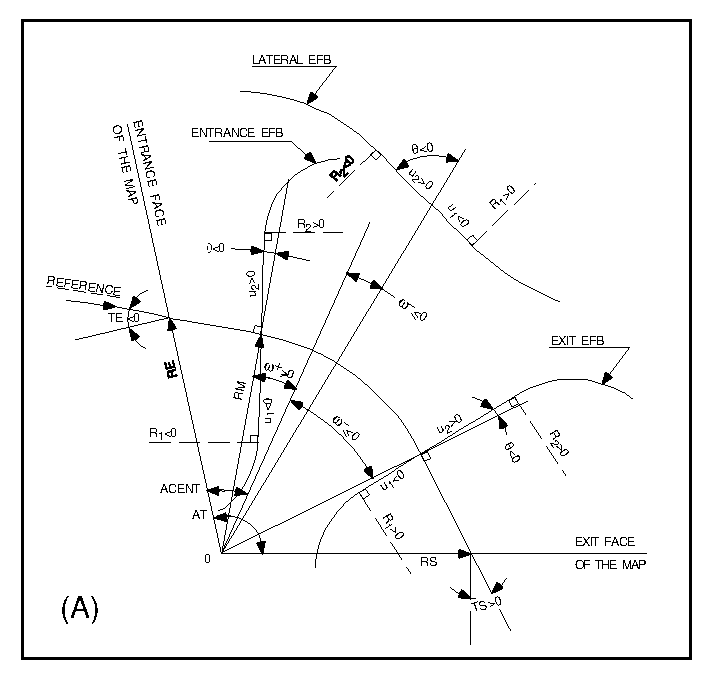
\includegraphics[width=12cm]{Fig9a.eps}
            \vfill
            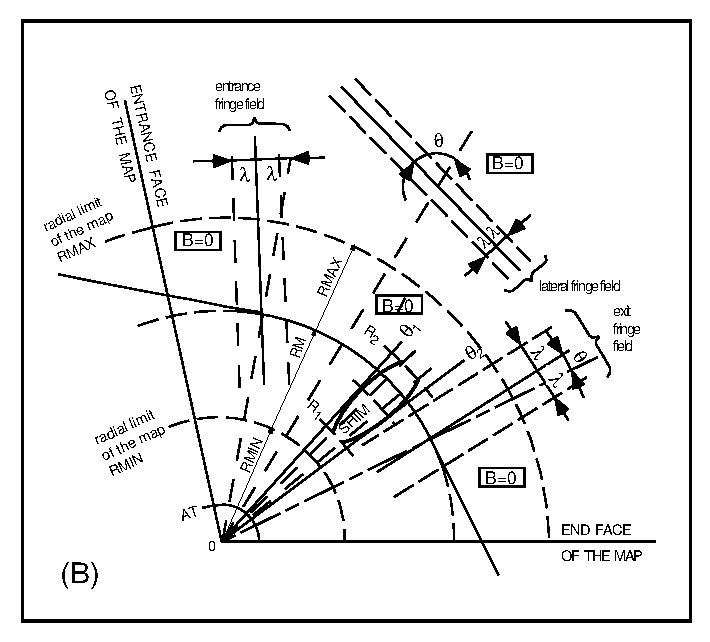
\includegraphics[width=12cm]{Fig9b.eps}
\medskip
\begin{center}
A : Parameters used to define the field map and geometrical boundaries.\\
B : Parameters used to define the field map and fringe fields.
\end{center}
\end{figure}


\newpage


\vfill 
%%%%%%%%%%%%%%figure%%%%%%%%%%%%%%
\begin{figure}[H]
%\vspace{9 truecm}
%%%Figure 10
\centerline{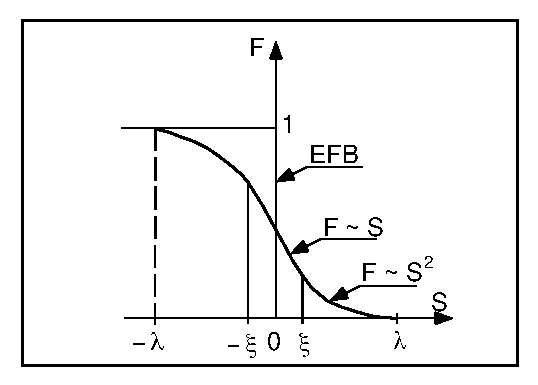
\includegraphics[width=10cm]{Fig10.ps}}
\unnumberedcaption{Second order type fringe field. }
\end{figure}
\vfill

%%%%%%%%%%%%%%figure%%%%%%%%%%%%%%
\begin{figure}[H]
%\vspace{11 truecm}
%%%Figure 11
\centerline{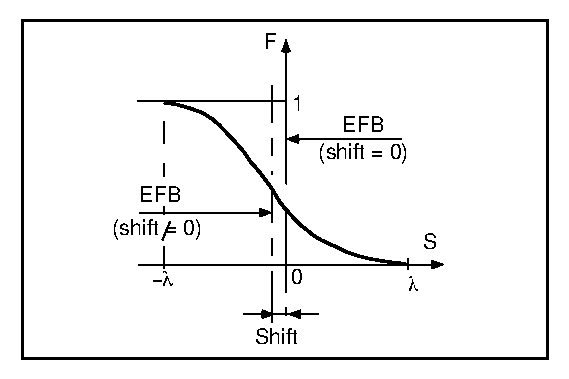
\includegraphics[width=10cm]{Fig11.ps}}
\unnumberedcaption{Exponential type fringe field.}
\end{figure}
\vfill 


\newpage

\begin{tabbing}  %% nouveaux tabs
\mestab
\textbf{AUTOREF} ~ ~ ~ ~  ~ ~ ~  ~ \quad \=   
1 : Equivalent to \textsl{CHANGREF} ($XCE=0$, 
		$YCE=Y(1)$, $ALE=T(1)$) ~ ~ ~ \quad   \quad \=  ~�~� 3*(1-\imax) \quad  \quad  \=\kill
\textbf{AUTOREF}  \label{AUTOREF-B} \index{AUTOREF|textbf}
  \> \textbf{\AUTOREFTitl} \\
 \\
 \\
$ I$             \> 1 : Equivalent to \textsl{CHANGREF}($XCE=0$, $YCE=Y(1)$, $ALE=T(1)$),  \> 1-2 \> I \\
                 \> \ie, recentering of the beam on particle \#1.                          \> 1-2 \> I \\
		 \\
 \> 2 : Equivalent to        \textsl{CHANGREF}($XW$, $YW$, $T(1)$), with ($XW$, $YW$) \> \> \\
 \> the location of the intersection (waist) of particles   1, 4 and 5 (useful \>\>\\
 \>  with \textsl{MATRIX}\index{MATRIX}, for automatic positioning of the first order focus). \>\>\\
 \\
 \> 3 : Equivalent to        \textsl{CHANGREF}($XW$, $YW$, $T(I1)$), with ($XW$, $YW$)  \\
 \>  the location of the intersection (waist) of particles $I1$, $I2$ and $I3$ (for  \>\>\\
 \> instance : $I1=$ central trajectory, $I2$  and $I3=$ paraxial trajectories \>\>\\
 \>that intersect at the first order  focus). \>\>\\
 \\
 \> 4 : Equivalent to        \textsl{CHANGREF}($XCE$, $YCE$, $ALE$).   \\
 \> 4.1 : Equivalent to        \textsl{CHANGREF}($XCE$, $YCE$, $ALE$) with in addition    \\
 \> centering of the beam on a new relative momentum  \textsl{DCE}.   \\
 \\
 \> 5 : The beam  is centered vertically on \textsl{ZCE, PLE}. \\
 \\
\textbf{If $I=3$}        \>Provide next record if $I=3$ \>\>\\
 $I1$, $I2$, $I3$      \>Three particle numbers \> 3*(1-\IMAX) \>3*I  \\
\\
\textbf{If $I=4$}        \>Provide next record  if $I=4$ \>\>\\
 \textsl{XCE, YCE, ALE} \> \XCE\ and beam centroid new coordinates \textsl{YCE, ALE}  \> 2*cm, mrad \>3*E  \\
 \\
\textbf{If $I=4.1$}        \>Provide next record  if $I=4.1$ \>\>\\
 \textsl{XCE, YCE, ALE,} \> \XCE\ and beam centroid new coordinates \textsl{YCE, ALE, DCE, TIME}  \> 2*cm, mrad,\> 6*E  \\
 \textsl{DCE, TIME} \>   \>   -, $\mu$s  \>  \\
 \\
\textbf{If $I=4.2$}        \>Provide next record  if $I=4.2$ \>\>\\
 \textsl{XCE, YCE, ALE,} \> \XCE\ and beam centroid new coordinates \textsl{YCE, ALE, DCE},  \> 2*cm, mrad,\> 6*E  \\
 \textsl{DCE, TIME} \>  time setting \textsl{TIME} (same for all particles). \>   -, $\mu$s  \>  \\
 \\
\textbf{If $I=5$}        \>Provide next record  if $I=5$ \>\>\\
 \textsl{ZCE, PLE} \> New vertical beam centroid coordinates \textsl{ZCE, PLE}  \> cm, mrad \>2*E  \\
 \\
\end{tabbing}



\newpage

\begin{tabbing}
\mestab
\textbf{BEAMBEAM} \label{BEAMBEAM-B} \index{BEAMBEAM|textbf} \index{beam-beam spin kick} \index{spin kick, beam-beam}
      \>\textbf{\BEAMBEAMTitl}\> \>    \\
\\
\\
SW, I   \> 0/1~: off/on~; beam intensity. \> 0-2, Amp   \> I, E  \\
  \>     Use \textsl{SPNTRK} to activate spin kicks.  \>  \>  \\
\\
$\alpha_Y, ~ \beta_Y, ~ \epsilon_{Y,norm}/\pi$   \> Beam parameters, horizontal.  \>  - , m, m.rad \> 3*E  \\
\\
$\alpha_Z, ~ \beta_Z, ~ \epsilon_{Z,norm}/\pi$   \> Beam parameters, vertical.  \>  - , m, m.rad \> 3*E  \\
\\
$\sigma_X, ~ \sigma_{dp/p}$   \> \rms\ bunch length~; \rms\ momentum spread.  \> m,  - \> 2*E  \\
\\
$\mathcal{C}, ~ \alpha$   \> Ring circumference~; momentum compaction. \> m, -  \>  2*E \\
\\
$Q_Y, ~ Q_Z, ~ Q_s$   \> Tunes, horizontal, vertical, synchrotron. \> -, -, -  \>  3*E  \\
\\
$A_Y, ~ A_Z, ~ A_X$   \> Amplitudes, horizontal, vertical, longitudinal. \>  -, -, -  \>  3*E  \\
\\
 \end{tabbing}




\newpage

\begin{tabbing}
\mestab
\textbf{BEND}  \label{BEND-B} \index{BEND|textbf} \>  \textbf{\BENDTitl} \> \> \\
 \\
 \\
 $\IL$   \>$\IL=1,2[\times 10^n],~7$ : print coordinates, fields, etc., along trajectories \>0-2$[\times 10^n]$, 7 \>I\\
        \> in zgoubi.res ($1$),  zgoubi.plt ($2$),  zgoubi.impdev.out ($7$).       \>                   \> \\
  \\
$ \XL$, $Sk$, $B1 $      \>Length~; skew angle~; field (change ALE and wedge signs, if B$<$0). \>cm, rad, kG \>3*E \\
  \\
 \>\textbf{Entrance face :}  \> \> \\
 $X_{\text{E}}$, $ \lambda_{\text{E}}$, $W_{\text{E}}$      \>Integration zone
extent~; fringe field extent (normally   $\simeq$ gap    height~;             \>cm, cm, rad \>3*E   \\
 \>  zero for sharp edge)~; wedge angle ($>$0 for rectangle magnet). \> \> \\
  \\
 $N$, $C_0$--$C_5$       \>Unused~; fringe field coefficients : $ B(s)=B1\, F(s)$ with   
 	\>unused, 6*no dim.\>I, 6*E \\
 \>$ F(s)=1/(1+ \exp(P(s)) $ and $ P(s)= \sum^ 5_{i=0}C_i(s/\lambda )^i$ \> \>\\
 \\
 \>\textbf{Exit face :} \> \> \\
 $X_S$, $\lambda_S $, $W_S$      \>See entrance face \> cm, cm, rad \> 3*E \\
 \\
 $N$, $C_0$--$C_5$        \> \>unused, 6*no dim. \>I, 6*E \\
 \\
 \textsl{XPAS}                 \>Integration step    \>cm \>E \\
 \\
 \textsl{KPOS, XCE, YCE, ALE}     \>\textsl{KPOS}=1 : element aligned, 2 : misaligned~; shifts, Z-tilt.
%  (unused if \textsl{KPOS}=1)
           \>1-2, 2*cm, rad \>I, 3*E \\
\> \textsl{KPOS} = 3 : \> \> \\
\> entrance and exit frames are shifted by \textsl{YCE} and tilted \wrt\ the magnet by an angle of           \> \> \\ 
\> $\bullet$ either ALE, if ALE is non-zero  (normally, ALE$>$0 in that case)\> \> \\ 
\> $\bullet$ or $2\, \textrm{Arcsin}( \Bone \times \XL\, /\, 2 \times \BORO)$ if ALE=0 \> \> \\ 

\end{tabbing}
%%%%%%%%%%%%%%figure%%%%%%%%%%%%%%
\begin{figure}[H]
%%%Figure 14
\centerline{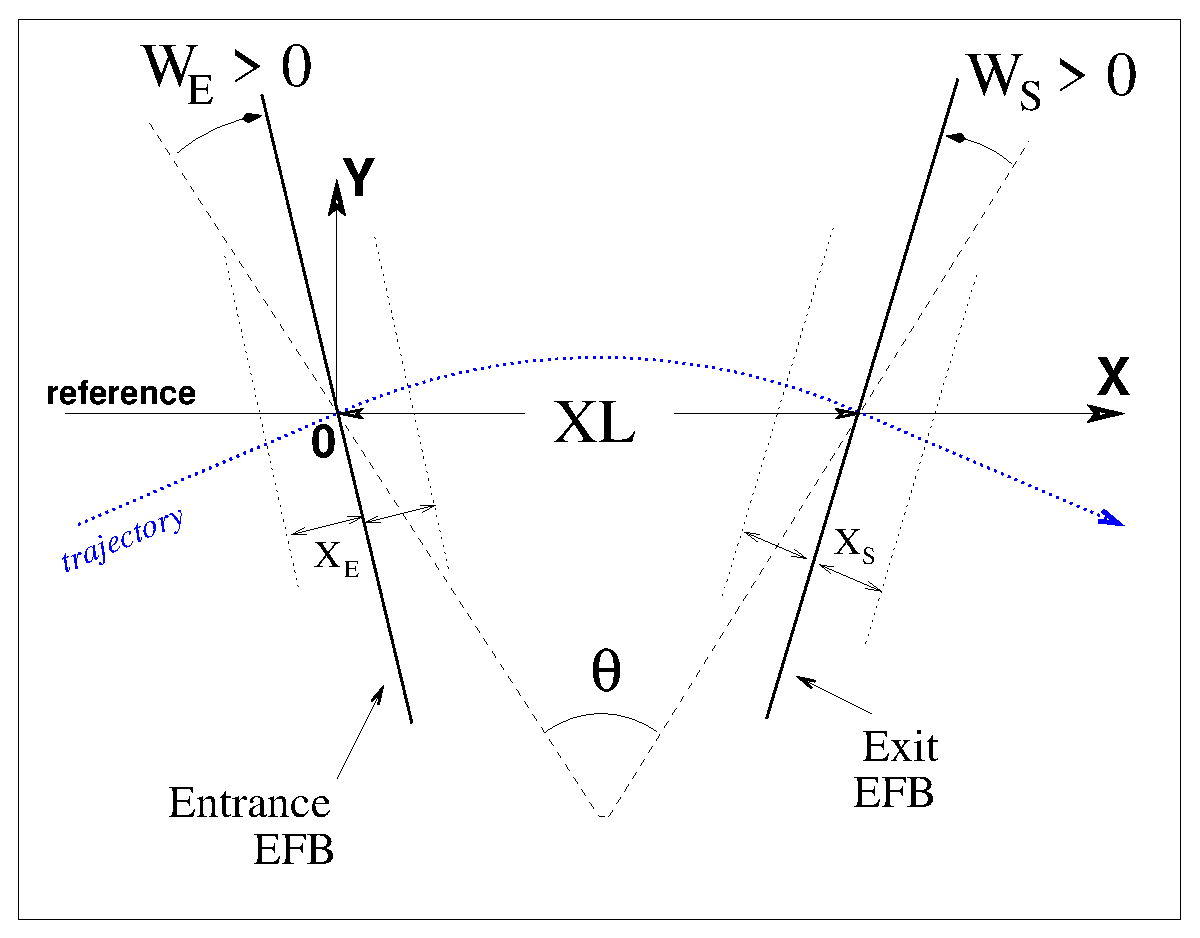
\includegraphics[height=6cm]{Fig14.eps}}
%\medskip

\begin{center}
\begin{minipage}[t]{8cm}
               \CapBEND
\end{minipage}
\end{center}
\end{figure}




\newpage

{\noindent $\bullet$ {\bf \textsl{Example}}~: Positive or negative field \textsl{BEND} \\ 

\smallskip

\noindent The data list at left hand, below, simulates a case of positive field, followed by two different ways 
to simulate the same magnet with negative field. (This can be copy-pasted to \zgou, as is, for execution.)

\noindent The right hand column shows the transport matrix in all three cases. 

\bigskip

\begin{minipage}{0.999\linewidth}
\begin{minipage}{0.45\linewidth}
{\tiny
\begin{verbatim}
Test signs, with wedges.
 
! Magnet deviation is
! tta=11.25deg=2asin(L/2rho)=2asin(B.L/2.Brho) with L=247.30039, Brho=1000, B=1.57776
 
! 1/ Positive B, regular form of input data
 'OBJET'                                                            
1000.
5
.01 .1 .01 .1 0. .001
0. 0. 0. 0. 0. 1.
 
 'BEND'                                                             
0
247.30039  0.  1.57776
20. 8. 0.04276056667                           ! wedge is +2.45deg
4 .2401  1.8639  -.5572  .3904 0. 0. 0.
20. 8. 0.04276056667                           ! wedge is +2.45deg
4 .2401  1.8639  -.5572  .3904 0. 0. 0.
#30|10|30
3 0. 0. -.1963495408
 
 'FAISCEAU'                                                         
 'MATRIX'                                                           
1 0
 
! 2/ Negative B. Compared to 1/ : R11-R44 unchaged, R16, R26 change sign.
! 2-a/ By changing sign of B. Note : signs of ALE and wedges have to be reversed.
 'OBJET'                                                            
1000.
5
.01 .1 .01 .1 0. .001
0. 0. 0. 0. 0. 1.
 
 'BEND'                                                             
0
247.30039  0.  -1.57776
20. 8. -0.04276056667                           ! wedge is +2.45deg
4 .2401  1.8639  -.5572  .3904 0. 0. 0.
20. 8. -0.04276056667                           ! wedge is +2.45deg
4 .2401  1.8639  -.5572  .3904 0. 0. 0.
#30|10|30
3 0. 0. .1963495408
 
 'FAISCEAU'                                                         
 'MATRIX'                                                           
1 0
 
! 2-a/ Using YMY instead. All data in BEND remain unchanged.
 'OBJET'                                                            
1000.
5
.01 .1 .01 .1 0. .001
0. 0. 0. 0. 0. 1.
 
 'YMY'                                                              
 'BEND'                                                             
0
247.30039  0.  1.57776
20. 8. 0.04276056667                           ! wedge is +2.45deg
4 .2401  1.8639  -.5572  .3904 0. 0. 0.
20. 8. 0.04276056667                           ! wedge is +2.45deg
4 .2401  1.8639  -.5572  .3904 0. 0. 0.
#30|10|30
3 0. 0. -.1963495408
 'YMY'                                                              
 
 'FAISCEAU'                                                         
 'MATRIX'                                                           
1 0
 
 'END'                                                              
\end{verbatim}
}
\end{minipage} ~ ~ ~ 
\begin{minipage}{0.49\linewidth}
{\tiny
\begin{verbatim}




  Reference particle (#     1), path length :   248.88547    

          TRANSFER  MATRIX  ORDRE  1  (MKSA units)
  0.940559         2.42528         0.00000         0.00000  0.0   0.482374    
 -4.768802E-02    0.940229         0.00000         0.00000  0.0   0.385904    
   0.00000         0.00000        0.985447         2.48908  0.0    0.00000    
   0.00000         0.00000       -1.163098E-02    0.985390  0.0    0.00000    
  0.385970        0.482384         0.00000         0.00000  1.0   6.370064E-02
   0.00000         0.00000         0.00000         0.00000  0.0    1.00000    













  Reference particle (#     1), path length :   248.88547    

          TRANSFER  MATRIX  ORDRE  1  (MKSA units)
  0.940559         2.42528         0.00000         0.00000  0.0  -0.482374    
 -4.768802E-02    0.940229         0.00000         0.00000  0.0  -0.385904    
   0.00000         0.00000        0.985447         2.48908  0.0    0.00000    
   0.00000         0.00000       -1.163098E-02    0.985390  0.0    0.00000    
 -0.385970       -0.482384         0.00000         0.00000  1.0   6.370064E-02
   0.00000         0.00000         0.00000         0.00000  0.0    1.00000    













  Reference particle (#     1), path length :   248.88547    

          TRANSFER  MATRIX  ORDRE  1  (MKSA units)
  0.940559         2.42528         0.00000         0.00000  0.0  -0.482374    
 -4.768802E-02    0.940229         0.00000         0.00000  0.0  -0.385904    
   0.00000         0.00000        0.985447         2.48908  0.0    0.00000    
   0.00000         0.00000       -1.163098E-02    0.985390  0.0    0.00000    
 -0.385970       -0.482384         0.00000         0.00000  1.0   6.370064E-02
   0.00000         0.00000         0.00000         0.00000  0.0    1.00000    
\end{verbatim}
}
\end{minipage} 
\end{minipage} 





\newpage
\begin{tabbing}
\mestab
\textbf{BINARY} \label{BINARY-B}\index{BINARY|textbf}
      \>\textbf{\BINARYTitl}\> \>    \\
\\
\\
$N\!F[.J], ~ N\!Col, ~ N\!H\!D\!R$	\> Number of files to convert [\texttt{READ} format type, see below],   \> $\leq20$, $\leq 7$ , $0-9$
                                                \> 3*I1 \\
                                        \>     of data columns,  of header lines.         \\
\\
\bf The next $N\!F$ lines : \> \> \\
\textsl{FNAME} \> Name of the file to be converted. File content  is assumed binary  \> \> A80 \\
	\> \textsl{iff} name begins with ``B$_{\_}$'' or ``b$_{\_}$'', assumed formatted otherwise.  \> \> \\
\\
\\
\\
\\
\\
\texttt{READ} format, case of formatted input file~: \\
\\
If FRM not given     \>   Format is '*' \\
If FRM=1             \>   Format is '1X, 7E11.*' \\
\\
\texttt{READ} format, case of binary input file~: \\
\\
Expected format is 7 column rows. \\
 \end{tabbing}




\newpage

\begin{tabbing}
\mestab
~ ~ $ \omega^+$, $\theta$,     $R_1$, $U_1$, $U_2$, $R_2 $     \quad \=
 �$ B=\mathcal{F}B_0 \left(1+N \left(\frac{R-RM }{ RM} \right)      
                +B \left(\frac{R-RM}{ RM} \right)^2+G \left(\frac{R-RM }{ RM}
                \right) \right) $, more    \quad \= 2*cm, 2*deg, cm ~ ~  \= \kill
%%%%
\textbf{BREVOL} \label{BREVOL-B}\index{BREVOL|textbf}
      \>\textbf{\BREVOLTitl}\> \>    \\
 \>$X$-axis cylindrical symmetry is assumed \>\>\\
 \\
 \\
 $\IC$, $\IL$      \>$\IC=1,2$ : print the map \>0-2; 0-2$[\times 10^n]$, 7 \>2*I\\
    \>$\IL=1,2[\times 10^n],~7$ : print coordinates, fields, etc., along trajectories \>   \>   \\
        \> in zgoubi.res ($1$),  zgoubi.plt ($2$),  zgoubi.impdev.out ($7$).       \>                   \> \\
% \>$\IL=1,2[\times 10^n]$ : print field and coordinates along trajectories.  \> \> \\
 \\
 \textsl{BNORM, XN}      \> Field and X-coordinate normalization  coeff.  \> 2*UnitConv. \> 2*E \\
        \> Convert values  as read from map file, to kG and cm units. \\
 \\
 \textsl{TITL}        \>Title. Start with ``FLIP'' to get field map X-flipped.  \> \>A80 \\
 \\
 $IX$       \>Number of longitudinal nodes of the map \> $\leq 400$ \> I \\
 \\
\textsl{FNAME [, SUM]}~\footnotemark[1]$^,$~\footnotemark[2]     \> File name  \> \>A80 \\
            \>   
 \\
 $ID$, $A$, $B$, $C$   \>Integration boundary. Ineffective when $ID=0$.      \>$\geq -1$, 2*no dim., \>I,3*E  \\
 {[}, $A'$, $B'$, $C'$,   \>$ID=$ -1, 1 or $\geq 2$ : as for  \textsl{CARTEMES} \> cm {[},2*no dim.,\>[,3*E,etc.]\\
 $B''$, etc., if $\left. ID\geq 2\right]$ \>                                  \> cm, etc.]       \> \\
  \\
 \textsl{IORDRE}     \> Unused \>2, 25 or 4 \>I\\
 \\
 \textsl{XPAS}          \>Integration step  \>cm \>E \\
 \\
 \textsl{KPOS}, \textsl{XCE},  \textsl{YCE, ALE}        \>\textsl{KPOS}=1 : element aligned, 2 : misaligned~; shifts, tilt. 
           \>1-2, 2*cm, rad \>I, 3*E \\
% \textsl{YCE, ALE}      \>shifts, tilt (unused if \textsl{KPOS}=1)  
 \end{tabbing}


\begin{alltt}
\footnotetext[1]{ \textsl{FNAME} (\emph{e.g.}, solenoid.map) \textrm{contains the field data. These must be formatted according to the following \textsl{FORTRAN} sequence :}  

	      OPEN (UNIT = NL, FILE = FNAME, STATUS = `OLD' [,FORM='UNFORMATTED'])
	      DO 1 I = 1, IX
	       IF (BINARY) THEN 
	              READ(NL) X(I), BX(I)
	       ELSE
	              READ(NL,*) X(I), BX(I)
	       ENDIF
         1     CONTINUE

\noindent \textrm{where \(X(I)\) and \(BX(I)\) are the longitudinal coordinate and field component at node \((I)\) of the mesh. Binary file names must begin with \textsl{FNAME}  'B\(\sb{_}\)' or 'b\(\sb{_}\)'. `Binary' will then automatically be set to `.TRUE.'.}} 
\end{alltt}  

\index{maps, summing} 
\begin{alltt}
\footnotetext[2]{ Sumperimposing (summing) field maps is possible. To do so, pile up file names with 'SUM' following each name but the last one. \emph{e.g.}, in the following example, 3 field maps are read and summed : 

myMapFile1  SUM
myMapFile2  SUM
myMapFile3  

\noindent (all maps must all have their mesh defined in identical coordinate frame). }
\end{alltt}  

\newpage
\begin{tabbing}  
\mestab
\textbf{CARTEMES} \label{CARTEMES-B} \index{CARTEMES|textbf}
        \>\textbf{\CARTEMESTitl}\> \> \\  
\>mid-plane symmetry is assumed \>\>\\
 \\
 \\
 $\IC$, $\IL$      \>$\IC=1,2$ : print  the map \>0-2; 0-2$[\times 10^n]$, 7 \>2*I\\
    \>$\IL=1,2[\times 10^n],~7$ : print coordinates, fields, etc., along trajectories \> \>   \\
        \> in zgoubi.res ($1$),  zgoubi.plt ($2$),  zgoubi.impdev.out ($7$).       \>                   \> \\
% \>$\IL=1,2[\times 10^n]$ : print field and coordinates along trajectories.  \> \> \\
 \\
 \textsl{BNORM, XN,YN}      \> Field and X-,Y-coordinate normalization  coeffs.     \> 3*UnitConv. \> 3*E \\
        \> Convert values  as read from map file, to kG and cm units. \\
 \\
 \textsl{TITL}        \>Title. Start with ``FLIP'' to get field map X-flipped.  \> \>A80 \\
 \\
 $IX$, $JY$      \>Number of longitudinal ($IX$) and transverse ($JY$) \>$\leq 400$, $\leq 200$ \>2*I \\
 \>nodes of the map \> \> \\
 \\
\textsl{FNAME}~\footnotemark[1] \> File name \> \>A80 \\
 \\
$ ID$\index{ID@{\textsl{ID}}|textbf}, $A$, $B$, $C$   \>Integration boundary. Normally $ID=0$.                   \>$\geq -1$,2*no dim.,\>I, 3*E\\  %
$\left[, A'\right.$, $B'$, $C'$, $A''$,\>$ID=-1$ : integration in the map begins at \>cm [,2*no dim., \>[3*E,etc.]\\ %
$B''$,etc., if $\left. ID\geq 2\right]$\>entrance boundary defined by $AX+BY+C=0$.\> cm, etc.]     \>           \\
                       \>$ID=1$ : integration in the map is terminated                \> \> \\
                       \>at exit boundary defined by $AX+BY+C=0$.                 \> \> \\
                       \>$ID \geq 2$ : entrance ($A, B, C$) and up to $ID-1$ exit  \> \> \\
                       \>($A', B', C', A'', B'', etc.$) boundaries                \> \> \\
 \\
 \textsl{IORDRE}     \>  Degree of interpolation polynomial (see \textsl{DIPOLE-M})   \>2, 25 or 4 \>I\\
 \\
 \textsl{XPAS}          \>Integration step  \>cm \>E \\
 \\
 \textsl{KPOS}, \textsl{XCE},  \textsl{YCE, ALE}       \>\textsl{KPOS}=1 : element aligned, 2 : misaligned~; shifts, tilt.  
           \>1-2, 2*cm, rad \>I, 3*E \\
% \textsl{YCE, ALE}      \>shifts, tilt (unused if \textsl{KPOS}=1)  
\end{tabbing}


\begin{alltt}
\footnotetext[2]{ \textsl{FNAME} (\emph{e.g.}, spes2.map) \textrm{contains the field data. These must be formatted according to the following \textsl{FORTRAN} sequence :} 

	      OPEN (UNIT = NL, FILE = FNAME, STATUS = `OLD' [,FORM='UNFORMATTED'])
	      IF (BINARY) THEN 
	        READ(NL) (Y(J), J=1, JY)
	      ELSE
                READ(NL,100) (Y(J), J=1, JY)
              ENDIF
     100      FORMAT(10 F8.2)	
              DO 1 I=1,IX
	        IF (BINARY) THEN 
	          READ(NL) X(I), (BMES(I,J), J=1, JY)
	      ELSE
	         READ(NL,101) X(I), (BMES(I,J), J=1, JY) 
     101	 FORMAT(10 F8.2)
              ENDIF
      1       CONTINUE

\textrm{where \(X(I)\) and \(Y(J)\) are the longitudinal and transverse coordinates and \textsl{BMES} is the \(Z\) field component  at a node \((I,J)\) of the mesh. For binary files, \textsl{FNAME} must begin with 'B\(\sb{_}\)' or 'b\(\sb{_}\)'. 
`Binary' will then automatically be set to `.TRUE.'}} 
\end{alltt}
\newpage
\vfill

%%%%%%%%%%%%%%figure%%%%%%%%%%%%%%
\begin{figure}[H]
%\vspace{19 truecm}
%%%Figure 15
\centerline{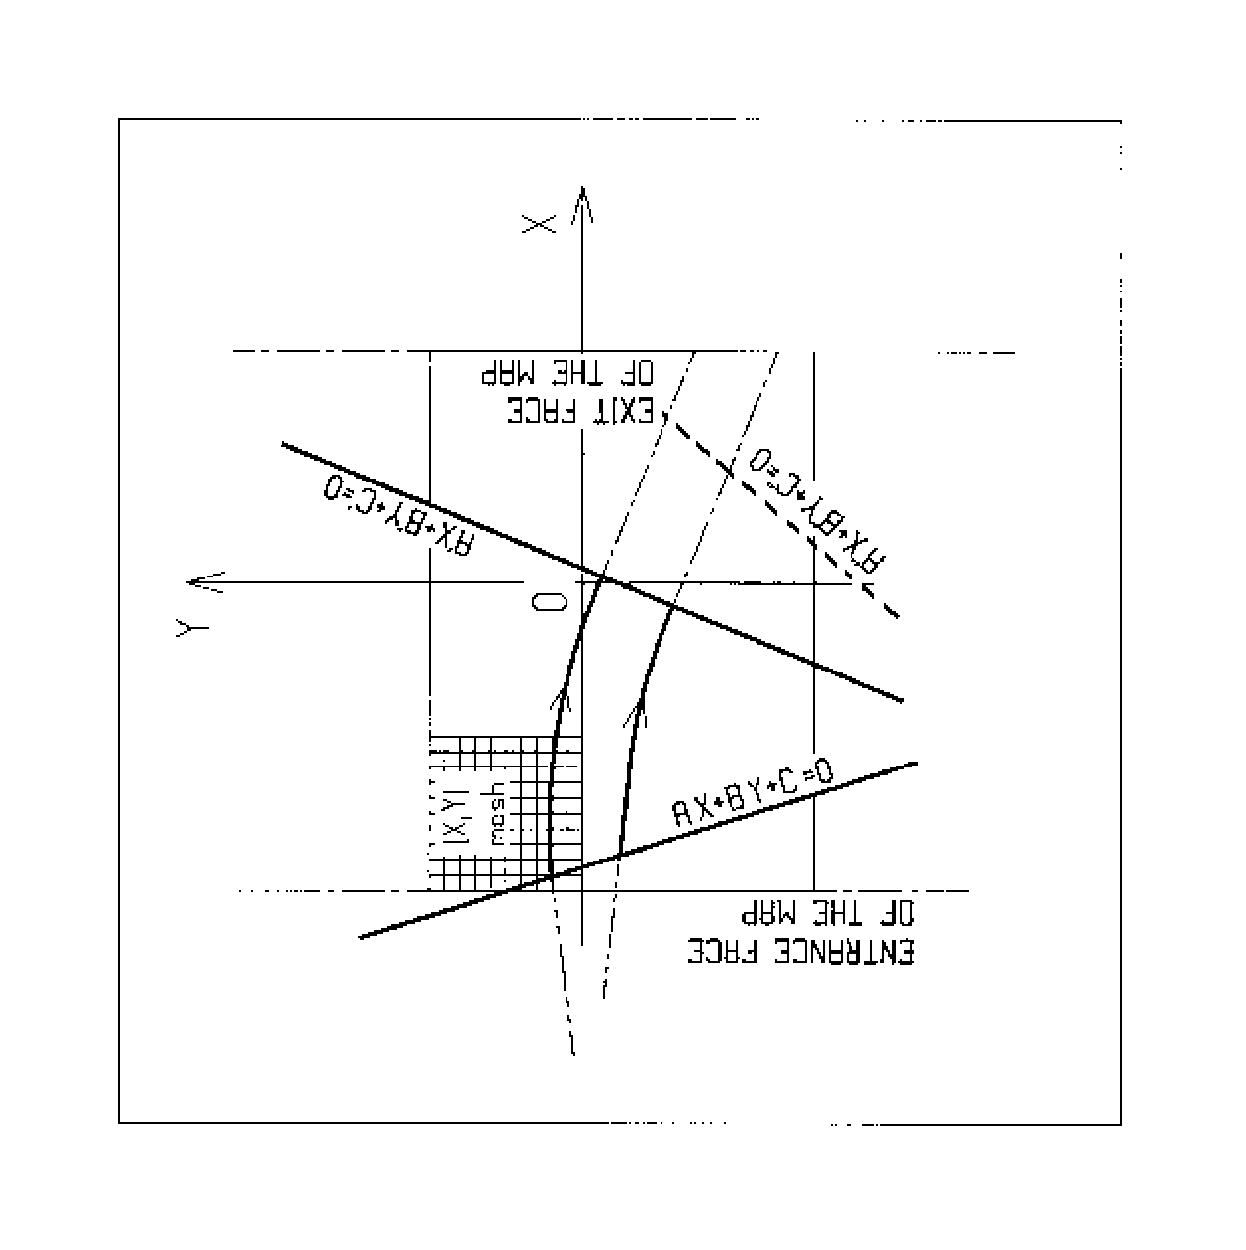
\includegraphics[height=15cm,angle=-90]{Fig15.ps}}
\unnumberedcaption{$OXY $ is the coordinate system of the mesh.
Integration zone limits may be defined, using $ ID\not= 0 $ : particle coordinates are
extrapolated linearly from the entrance face of the map, into the plane 
$A'X+B'Y+C'=0$~; after ray-tracing inside the 
map and terminating on the integration boundary $AX+BY+C=0$,   coordinates are
extrapolated linearly to the exit face of the map.}
\end{figure}
\vfill

\newpage

\begin{tabbing}
\mestab
~ ~ $ \omega^+$, $\theta$,     $R_1$, $U_1$, $U_2$, $R_2 $     \quad \=
 �$ B=\mathcal{F}B_0 \left(1+N \left(\frac{R-RM }{ RM} \right)      
                +B \left(\frac{R-RM}{ RM} \right)^2+G \left(\frac{R-RM }{ RM}
                \right) \right) $, more  \quad  \quad  \quad \= 2*cm, 2*deg, cm   \= \kill
%%%%%
\textbf{CAVITE~\footnotemark[1]} \label{CAVITE-B} \index{CAVITE|textbf}\index{acceleration}\index{synchrotron motion}
     \> \textbf{\CAVITETitl}   \> \> \\
 \> $ \Delta W=qVsin(2\pi hf\Delta t+\varphi_ s) $ and other voltage and frequency laws.   \> \> \\
 \\
 \\
 \textsl{IOPT[.i]}       \> Option. $i=1$ causes info output into \texttt{zgoubi.CAVITE.Out}    \>0-7 \>I \\
 \\
\textbf{If IOPT=0}  \>Element inactive \>\>\\
\\
$ X$, $X $        \> Unused. \>\>\\
$ X$, $X $        \> Unused. \>\>\\
  \\
\textbf{If IOPT=1}~\footnotemark[2]  \> $ f_{RF} $ follows the timing law given by \textsl{SCALING}\index{SCALING}\\
 \\
$\mathcal{L}$, $h$       \> Reference closed orbit length~; harmonic number. \>m, no dim.  \>2*E\\
$ \hat  V, ~ X $       \> R.F. peak voltage~; unused.  \>V, unused\>2*E\\
 \\
\textbf{If IOPT=2}  \> $ f_{RF} $ follows $ \Delta W_s=q\hat  Vsin\phi_ s $ \\
 \\
$\mathcal{L}$, $h $      \> Reference closed orbit length~; harmonic number. \>m, no dim.\>2*E\\
$ \hat  V$, $\phi_ s $       \> R.F. peak voltage~; synchronous phase. \>V, rad \>2*E\\
 \\
\textbf{If IOPT=3}  \> No synchrotron motion : $ \Delta W=q\hat  Vsin\phi_ s $ \> \> \\
\\
$ X$, $X$       \> Unused~; unused.   \> 2*unused. \> 2*E\\
$ \hat  V$, $\phi_ s $       \>R.F. peak voltage~; synchronous phase. \>V, rad \>2*E \\
 \\
\textbf{If IOPT=6}  \> Read  RF frequency and/or phase law from  external file, ``zgoubi.freqLaw.In''.  \\
\\
$\mathcal{L}$, $E_k$       \> Orbit length and kinetic energy at start of acceleration.  \>  m, MeV  \>  2*E  \\
$ \hat  V, ~ \Phi_s $       \> R.F. peak voltage~; synchronous phase. \> V, rad \> 2*E \\
 \\
\textbf{If IOPT=7}  \>   Quasi- or isochronous acceleration. \\
\\
$X$, $f_{RF}$       \> Unused~; RF frequency.   \>  - , Hz  \>  2*E  \\
$ \hat  V, ~ \Phi_s $  \> R.F. peak voltage~; synchronous phase. \> V, rad \> 2*E \\
 \\
\textbf{If IOPT=10}  \>   Chambers matrix method. \\
\\
$L$, $f_{RF}$       \> Cavity length~; RF frequency.   \>  m , Hz  \>  2*E  \\
$ \hat  V, ~ \Phi_s $, \textsl{IOPT}  \> R.F. peak voltage~; synchronous phase~; matrix options. \> V, rad, $-2$-$2$ \> 2*E, I \\
%$ \hat  V, ~ \Phi_s $, \textsl{IOPT}  \> R.F. peak voltage~; synchronous phase~; matrix options~; $B\rho_{ref}$ setting. \> V, rad, $-2$-$2$, - \> 2*E, I, E \\


\end{tabbing}

\footnotetext[1]{~ Use \textsl{PARTICUL} to declare mass and charge. }
\footnotetext[2]{~ For ramping the R.F. frequency following 
$ B\rho (t)$,  use \textsl{SCALING}, with family \textsl{CAVITE}. } 




\newpage

\begin{tabbing}
\mestab
~ ~ $ \omega^+$, $\theta$,     $R_1$, $U_1$, $U_2$, $R_2 $     \quad \=
 �$ B=\mathcal{F}B_0 \left(1+N \left(\frac{R-RM }{ RM} \right)      
                +B \left(\frac{R-RM}{ RM} \right)^2+G \left(\frac{R-RM }{ RM}
                \right) \right) $, more  \quad  \quad  \= 2*cm, 2*deg, cm   \= \kill
%%%%%
\textbf{CHAMBR}  \label{CHAMBR-B} \index{CHAMBR|textbf} 
        \> \textbf{\CHAMBRTitl~\footnotemark[1]}
\\
\\
 $IA$          \>0 : element inactive \> \> \\
 \>1 : (re)definition of the aperture   \> 0-2 \> I \\
 \>2 : stop testing and reset counters, print \> \> \\
 \>information on stopped particles\index{stopped particles}. \> \> \\
 \\
 \textsl{IFORM[.J]}, $C1$, $C2$,\>\textsl{IFORM} = 1 : rectangular aperture~;  \>1-2[.0-1] \> I[.I], 4*E \\
                   $C3$, $C4$   \>\textsl{IFORM} = 2 : elliptical aperture. \>\>\\
                                \>\textsl{J} = 0, default : opening is~\footnotemark[2] ~ $\pm \YL=\pm C1$, $\pm \ZL=\pm C2$,  \>\>\\
                                \> centered at $\YC=C3$, $\ZC=C4$. \>\>\\
                                \>\textsl{J} = 1 : opening is~\footnotemark[2], in Y~: $[C1,C2]$, in Z~: $[C3,C4]$ \>\>\\
\\
% \textsl{IFORM, YL$~\footnotemark[2]$, ZL, YC, ZC} \>Taken into account only if $IA=1$.
%      \>1-2, 4*cm \>I, 4*E \\
% \>\textsl{IFORM} = 1 : rectangular chamber~; horizontal\> \> \\
% \>(vertical) dimension $\pm YL$ ($\pm ZL$)~; \> \> \\
% \>centered at $YC$, $ZC$. \> \> \\
% \>\textsl{IFORM} = 2 : elliptical chamber~; horizontal \>\>\\
% \>(vertical) axis $\pm YL$($\pm ZL$)~; \>\>\\
% \>centered at $YC$, $ZC$.  
\end{tabbing}

\footnotetext[1]{~ Any particle out of limits is stopped\index{stopped particles}. }
\footnotetext[2]{~ When used with an optical element 
defined in polar coordinates (\emph{e.g.}, \textsl{DIPOLE}) $YL$ is the radius and  
$YC$ stands for the reference radius (normally, $YC  \simeq RM$).} 

\newpage

\begin{tabbing}
\mestab
\textbf{CHANGREF}  \label{CHANGREF-B} \index{CHANGREF|textbf}      \> \textbf{\CHANGREFTitl}\\
 \\
 \textbf{``Old Style''} (Figure below)~: \index{CHANGREF ``Old Style''}  \\
\\
 \textsl{XCE, YCE, ALE} \>Longitudinal and transverse shifts, \>2*cm, deg \>3*E \\
 \>followed by $Z$-axis rotation  \\
\\
\\
 \textbf{``New Style'' (example below). \index{CHANGREF ``New Style''}  In an arbitrary order, up to 9  occurrences of~:  }\\
\\
 \textsl{XS 'val', YS 'val', ZS 'val',} \> \>cm or deg \>up to 9*(A2,E) \\
 \textsl{XR 'val', YR 'val', ZR 'val'} \> \>\>\\
\end{tabbing}
\vfill

%% figure 16
%%%%%%%%%%%%%%figure%%%%%%%%%%%%%%
\begin{figure}[H]
%\vspace{10.5 truecm}
%%%Figure 16
\centerline{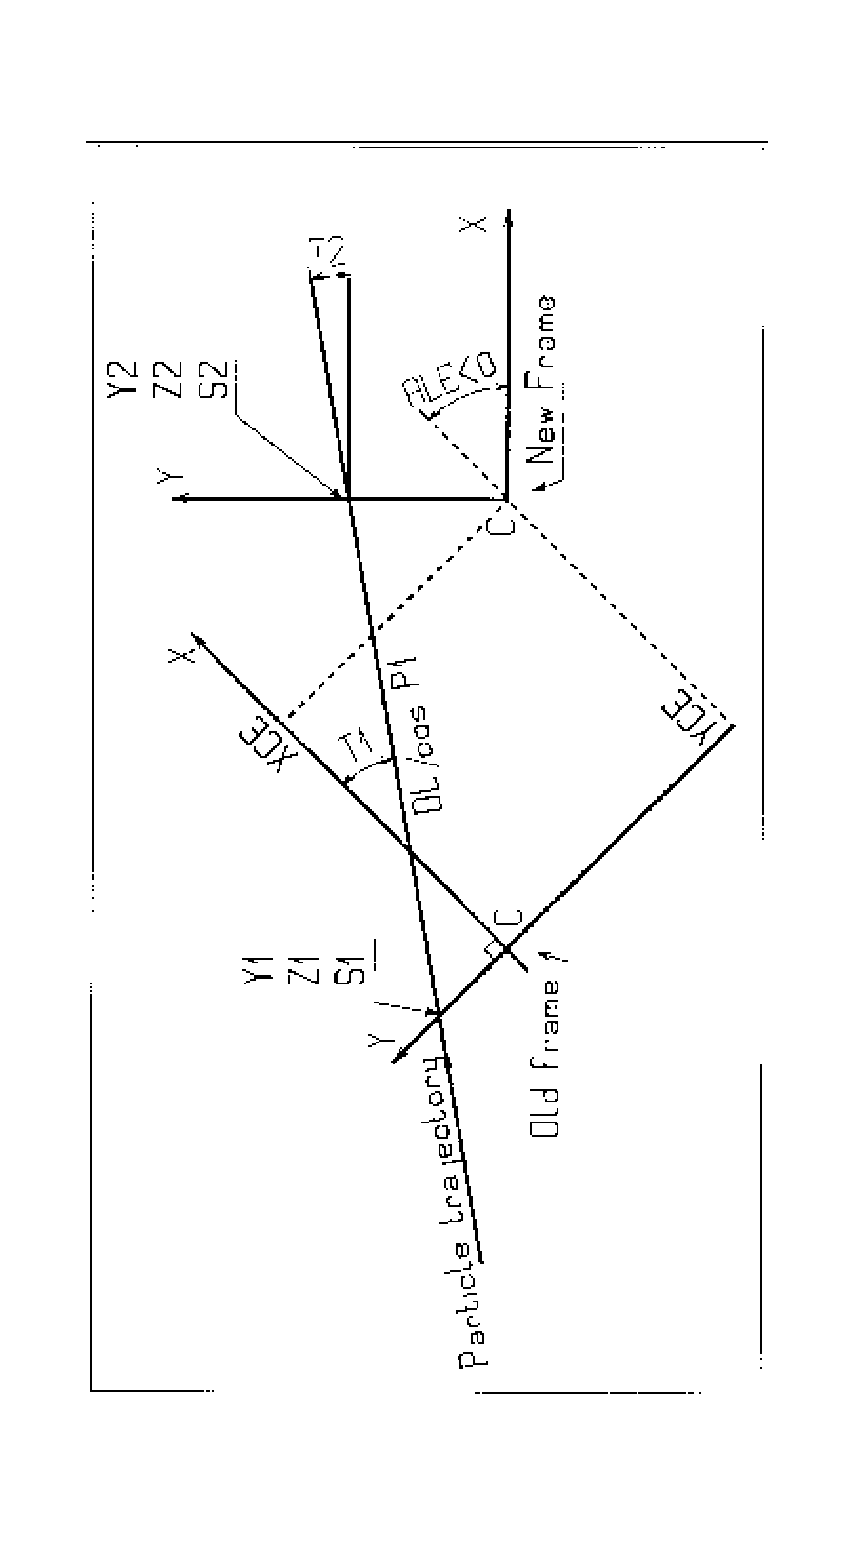
\includegraphics[height=12cm,angle=-90]{FigCHAREFa.eps}}
\unnumberedcaption{Parameters in the \CHANGREF\ procedure. }
\end{figure}


\medskip

Example~: 

\begin{center}
\begin{minipage}{.38\linewidth}
\footnotesize
\begin{verbatim}
Using CHANGREF "New Style
'OBJET'
51.71103865921708                          Electron, Ekin=15MeV.
2
1 1                                           One particle, with
2. 0.  0.0 0.0 0.0 1. 'R'      Y_0=2 cm, other coordinates zero.
1 1 1 1 1 1 1 
'MARKER'    BEG    .plt                -> list  into zgoubi.plt.
'DRIFT'                                             10 cm drift.
10.
'CHANGREF'  
ZR -6.34165 YS 1.             First half Z-rotate, Next Y-shift.
'MULTIPOL'     Combined function multipole, dipole + quadrupole.
   2                                   -> list  into zgoubi.plt.
5  10. 2.064995867082342  2. 0. 0. 0. 0. 0. 0. 0. 0.
 0 0  5. 1.1  1.00 1.00 1.00 1.00 1.00 1. 1. 1. 1.                              
4  .1455   2.2670  -.6395  1.1558  0. 0.  0.                                    
 0 0  5. 1.1  1.00 1.00 1.00 1.00 1.00 1. 1. 1. 1.                              
4  .1455   2.2670  -.6395  1.1558  0. 0.  0.                                    
0 0 0 0 0 0 0 0 0 0
.1   step size
1  0. 0.  0.
'CHANGREF'
YS -1. ZR -6.341         First Y-shift back, next half Z-rotate.
'DRIFT'                                             10 cm drift.
10.
'FAISCEAU'
'END'
\end{verbatim}
\normalsize
\end{minipage}\hspace{.05\linewidth}
\end{center}



\vfill



\newpage

\begin{tabbing}
\mestab
\textbf{CIBLE, TARGET}         \label{CIBLE-B} \index{CIBLE|textbf} \label{TARGET-B} \index{TARGET|textbf}
     \> \textbf{\CIBLETitl} \>\>\\
 \\
 \\
$ M_1$, $M_2$, $M_3$, $Q $        \>Target, incident and scattered particle masses~; 
             \>5*$ \dfrac{MeV}{c^2}$, 2*deg \> 7*E \\
$ T_2$, $\theta$, $\beta $            \>$ Q $ of the reaction~; incident particle kinetic \>\>\\
 \>energy~; scattering angle~; angle of the target \>\>\\
 \\
 $NT$, $NP$             \>Number of samples in $T$ and $P$ coordinates \> \>2*I\\
 \>after \textsl{CIBLE} \>\>\\
 \\
 $TS$, $PS$, $DT$          \>Sampling size~; tilt angle \>3*mrad \>3*E \\
 \\
 \BORO\index{BORO@{\BORO}}              \>New reference rigidity after  \textsl{CIBLE}  \>kG.cm \>E
\end{tabbing}
\vfill

%%%%%%%%%%%%%%figure%%%%%%%%%%%%%%
\begin{figure}[H]
%\vspace{17 truecm}
%%%Figure 17
\centerline{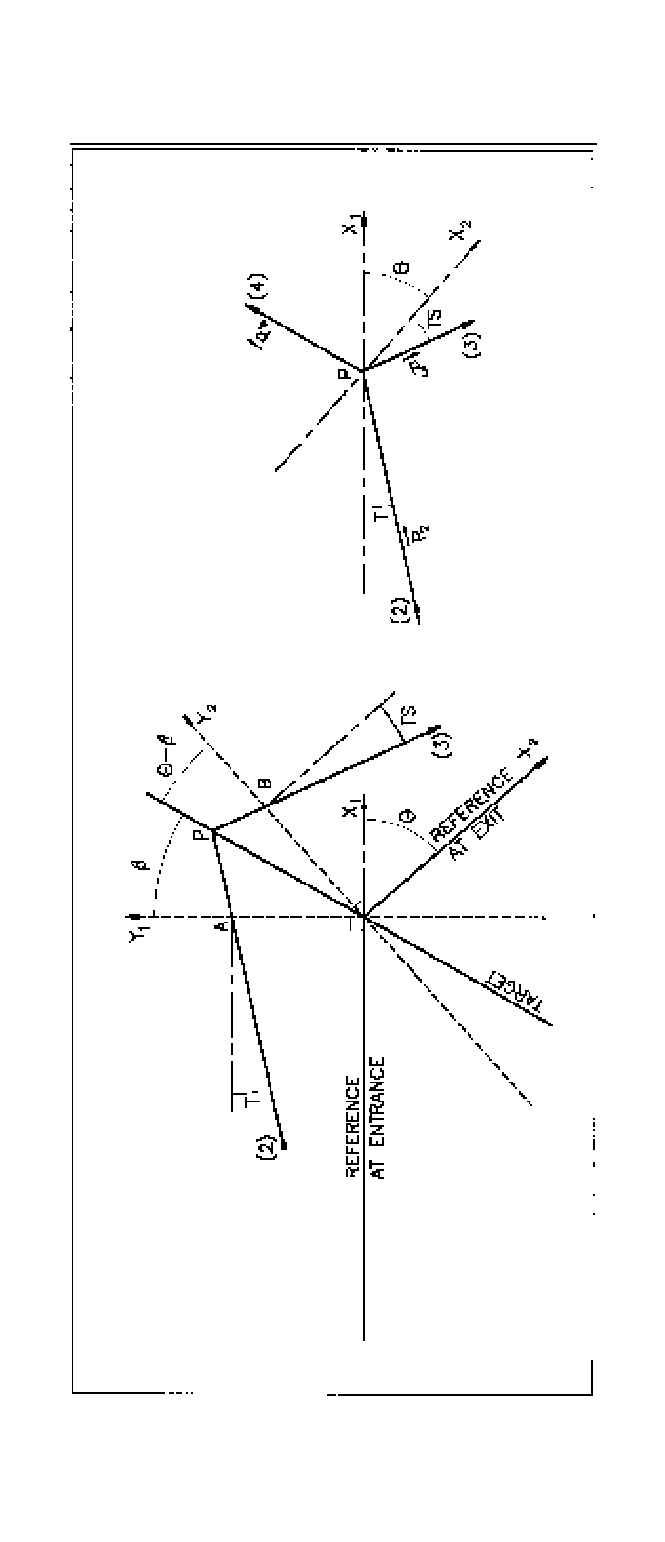
\includegraphics[height=15cm,angle=-90]{Fig17.ps}}
\unnumberedcaption{Scheme of the principles of \textsl{CIBLE (TARGET)}} 
\begin{center}
	\begin{minipage}[t]{13cm}
$ A, T$   =   position, angle of incoming particle 2 in the entrance reference frame\\
$	P$   =   position of the interaction\\
$B, T$   =   position, angle of the secondary particle  in the exit reference frame\\ 
$\theta$   =   angle between entrance and exit frames\\
$\beta$   =   tilt angle of the target 
	\end{minipage} 
\end{center}

\end{figure}
\vfill

\newpage

\begin{tabbing}
\mestab
~ ~ $ \omega^+$, $\theta$,     $R_1$, $U_1$, $U_2$, $R_2 $     \quad \=
 �$ B=\mathcal{F}B_0 \left(1+N \left(\frac{R-RM }{ RM} \right)      
                +B \left(\frac{R-RM}{ RM} \right)^2+G \left(\frac{R-RM }{ RM}
                \right) \right) $, more  \quad  \quad  \= 2*cm, 2*deg, cm \quad \quad  \= \kill
%%%%%
\textbf{COLLIMA}         \label{COLLIMA-B} \index{COLLIMA|textbf}
         \> \textbf{\COLLIMATitl}~\footnotemark[1]   \> \> \\
 \\
 \\
 $IA$       \> 0 : element inactive \> \> \\
 \> 1 : element active   \>0-2 \>I \\
 \> 2 : element active and print information on stopped 
 \\
 \>particles\index{stopped particles} \>\>\\
 \\
\textbf{Physical-space collimation} 
\\
% \textsl{IFORM}, $\YL$, $\ZL$,  \>\textsl{IFORM} = 1 : rectangular collimator~; horizontal \>1-2, 4*cm \> I, 4*E \\
%$\YC$, $\ZC$  \>(vertical) dimension $\pm \YL$ ($\pm \ZL$)~; \>\>\\
 \textsl{IFORM[.J]}, $C1$, $C2$,\>\textsl{IFORM} = 1 : rectangular aperture~;  \>1-2[.0-1] \> I[.I], 4*E \\
                   $C3$, $C4$   \>\textsl{IFORM} = 2 : elliptical aperture. \>\>\\
                                \>\textsl{J} = 0, default : opening is $\pm \YL=\pm C1$, $\pm \ZL=\pm C2$,  \>\>\\
                                \> centered at $\YC=C3$, $\ZC=C4$. \>\>\\
                                \>\textsl{J} = 1 : opening is, in Y~: $[C1,C2]$, in Z~: $[C3,C4]$ \>\>\\
\\
\textbf{Longitudinal  collimation} 
\\
 \textsl{IFORM.J}, $H_{min}$, $H_{max}$,\>\textsl{IFORM} = 6 or 7 for horizontal 
          variable resp$^\textrm{ly}$ S  or Time, \> 2*cm or 2*$�$s, \> I, 4*E \\
$V_{min}$, $V_{max}$  \> J=1 or 2 for vertical variable resp$^\textrm{ly}$ 1+dp/p, kinetic-E (MeV)~;   \> 2*no.dim or 2*MeV\>\\
                \> horizontal and vertical   limits \>\>\\
\\
\textbf{Phase-space collimation} 
\\
\textsl{IFORM}, $\alpha$, $\beta$, $\epsilon/\pi$, $N_{\sigma}$ \>\textsl{IFORM} = 11, 14 : horizontal collimation~; 
                                                 horizontal \>11-16, no.dim,   \>I, 4*E \\
  \> ellipse parameters (unused if 14)~\footnotemark[2], emittance, cut-off  \>  2*m, no.dim\>\\
 \>\textsl{IFORM} = 12, 15 : vertical collimation~; vertical \>\>\\
 \>ellipse parameters (unused if 15)~\footnotemark[2], emittance, cut-off  \>\> \\
 \>\textsl{IFORM} = 13, 16 : longitudinal collimation~; \textsl{to be } \>\>\\
 \> \textsl{implemented}
\end{tabbing}

\footnotetext[1]{~ Any particle out of limits is stopped\index{stopped particles}.} 

\footnotetext[2]{~ The rejection boundary is the \rms\ ellipse matched to the particle distribution.}


\newpage

\begin{tabbing}
\mestab
\textbf{DECAPOLE}         \label{DECAPOLE-B} \index{DECAPOLE|textbf}
  \> \textbf{\DECAPOLETitl}   \> \> \\
  \\
  \\
 $\IL$   \>$\IL=1,2[\times 10^n],~7$ : print coordinates, fields, etc., along trajectories \>0-2$[\times 10^n]$, 7 \>I\\
        \> in zgoubi.res ($1$),  zgoubi.plt ($2$),  zgoubi.impdev.out ($7$).       \>                   \> \\
% $\IL$        \> $\IL=1,2[\times 10^n]$ : print field and coordinates along trajectories.  \>0-2$[\times 10^n]$ \>I \\
 \\
 $\XL$, $R_0$, $B_0 $ \>Length~; radius and field at pole tip  \>2*cm, kG \>3*E \\
 \\
 \>Entrance face : \>\>\\
$ X_E$, $\lambda_ E $    \>Integration zone extent~; fringe field  \>2*cm \>2*E \\
 \>extent ($\losim 2  R_0$, $\lambda_ E=0 $ for sharp edge) \>\>\\
 \\
 \textsl{NCE}, $ C_0-C_5 $ \> \textsl{NCE} = unused \>unused,  \>I, 6*E \\
 \>$ C_0-C_5 $ = Fringe field coefficients such that \> 6*no dim.\> \\
 \>$ G(s)=G_0/(1+ \exp  P(s))$,  with $ G_0=B_0/R^4_0 $ \>\>\\
 \>and $ P(s) = \sum^ 5_{i=0}C_i(s/\lambda )^i $ \>\>\\
 \\
$ X_S$, $\lambda_ S $    \>Exit face : see entrance face \>2*cm \>2*E \\
 \textsl{NCS}, $ C_0-C_5 $ \> \>0-6, 6*no dim. \>I, 6*E \\
 \\
 \textsl{XPAS}          \>Integration step  \>cm \>E \\
 \\
 \textsl{KPOS, XCE, YCE, ALE}    \>\textsl{KPOS}=1 : element aligned, 2 : misaligned~; shifts, tilt.  
           \>1-2, 2*cm, rad \>I, 3*E \\
%       \>shifts, tilt (unused if \textsl{KPOS}=1)  
\end{tabbing} 
\vfill

%%%%%%%%%%%%%%figure%%%%%%%%%%%%%%
\begin{figure}[H]
%\vspace{12 truecm}
%%%Figure 18
\centerline{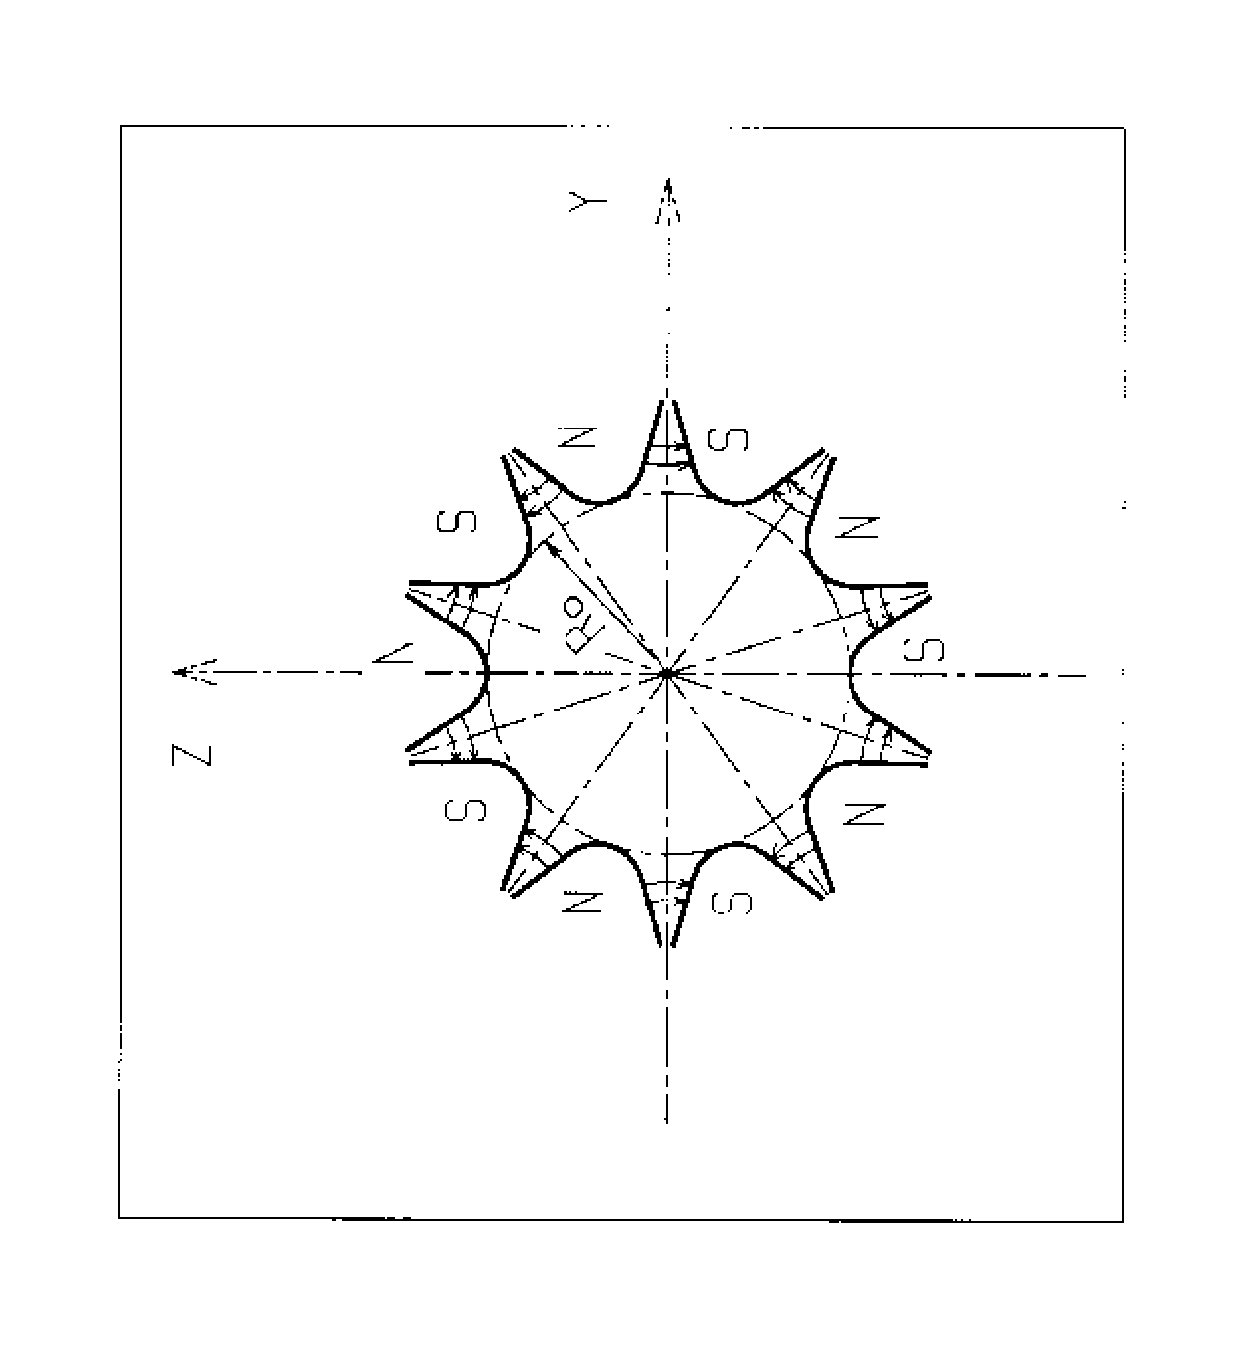
\includegraphics[height=10cm,angle=-90]{Fig18.ps}}
%%\hangcaption{\label{fig18}Decapole magnet}
\end{figure}
\vfill



\newpage

\begin{tabbing}
\mestab
~ ~ $ \omega^+$, $\theta$,     $R_1$, $U_1$, $U_2$, $R_2 $     \quad \=
 �$ B=\mathcal{F}B_0 \left(1+N \left(\frac{R-RM }{ RM} \right)      
                +B \left(\frac{R-RM}{ RM} \right)^2+G \left(\frac{R-RM }{ RM}
                \right) \right) $, more  \quad  \quad  \= 2*cm, 2*deg, cm \quad \quad   \= \kill
%%%%%
\textbf{DIPOLE}         \label{DIPOLE-B} \index{DIPOLE|textbf}
           \>\textbf{\DIPOLETitl}\> \>\\
 \>$ B_Z= \mathcal{F} B_0 \left(1 + N \left(\dfrac{R-RM}{RM} \right) +B 
 \left(\dfrac{R-RM}{RM} \right)^2+G \left(\dfrac{R-RM}{RM} \right)^3 \right) $ \> \> \\
 \\
 \\
 $\IL$   \>$\IL=1,2[\times 10^n],~7$ : print coordinates, fields, etc., along trajectories \>0-2$[\times 10^n]$, 7 \>I\\
        \> in zgoubi.res ($1$),  zgoubi.plt ($2$),  zgoubi.impdev.out ($7$).       \>                   \> \\
% $\IL$    \>$\IL=1,2[\times 10^n]$ : print field and coordinates along trajectories.\> 0-2$[\times 10^n]$ \>  I  \\
 \\
 $AT$,  $RM$       \> Total angular extent  of the dipole~;  reference radius \> deg, cm \> 2*E\\
 \\
 \textsl{ACENT}, $ B_0$, $N$, $B$, $G $           \>
 Azimuth for positioning of EFBs~; field and field indices \> deg., kG, 3*no dim.  \> 5*E\\
% \>                        \> 3*no dim. \> \\
 \\
 \>ENTRANCE FIELD BOUNDARY \> \> \\
 \\
$\lambda$, $\xi$               \>Fringe field extent (normally $\simeq$ gap size)~; unused. 
           \> cm, unused \>2*E\\
 \>Exponential type fringe field $ F=1\, /\, (1+ \exp (P(s)))$   \>\>\\
 \>with $ P(s)=C_0+C_1(\dfrac{s}{\lambda} )+C_2(\dfrac{s}{\lambda} )^2
             +...+C_5(\dfrac{s}{\lambda} )^5 $   \>\>\\
 \\
 $NC$, $ C_0-C_5 $, shift     \>Unused~; $ C_0 $ to $ C_5 $ : see above~; EFB shift  \>0-6, 6*no dim., cm  \>I, 7*E\\
% \>EFB shift   \>no dim., cm \> \\
\\
$ \omega^ +$, $\theta$, $R_1$, $U_1$, $U_2$, $R_2 $   \>Azimuth of entrance EFB with respect
         to \textsl{ACENT}~; \>2*deg, 4*cm 
\>6*E\\
 \>wedge angle of EFB~; radii and linear \> \> \\
 \>extents of EFB (use $\mid  U_{1,2}  \mid  = \infty$ when $R_{1,2}=\infty$)  \>\>\\
 \\
% \>(Note : $ \lambda =0$, $\omega^ + $ = \textsl{ACENT} and $ \theta =0 $ for
%         \underbar{sharp edge}) \>\>\\
% \\
 \>EXIT FIELD BOUNDARY (See ENTRANCE FIELD BOUNDARY) \>\>\\
 \\
$\lambda$, $\xi$               \>Fringe field parameters \>cm, unused\>2*E \\
 $NC$, $ C_0-C_5 $, shift     \>    \>0-6, 6*no dim., cm \>1, 7*E\\
% \>    \>dim., cm \> \\
\\
$ \omega^-$, $\theta$, $R_1$, $U_1$, $U_2$, $R_2 $   \>Positioning and shape of the
              exit EFB \>2*deg, 4*cm \>6*E\\
 \\
% \>(Note : $ \lambda =0$, $\omega^- = -AT+$ \textsl{ACENT} and $ \theta 
% =0 $ for \> \> \\
%\> \underbar{sharp edge})
 \\
 \>LATERAL FIELD BOUNDARY (See ENTRANCE FIELD BOUNDARY) \>\>\\
 \\
$\lambda$, $\xi$               \> LATERAL EFB is inhibited if $\xi=0$\>cm, unused\>2*E \\
 $NC$, $ C_0-C_5 $, shift     \>    \>0-6, 6*no dim., cm \>1, 7*E\\
$ \omega^-$, $\theta$, $R_1$, $U_1$, $U_2$, $R_2 $,    \>Positioning and shape of the EFB \>2*deg, 5*cm \>7*E\\
$ RM3$   \> \> \> \\
 \\
% \>(Note : $ \lambda =0$, $\omega^- = -AT+$ \textsl{ACENT} and $ \theta 
% =0 $ for \> \> \\
%\> \underbar{sharp edge}) \\
  \\
 \textsl{IORDRE, Resol}  \> Degree of interpolation polynomial :        \> 2, 25 or 4~; no dim. \>I, E\\
 \>\ 2 = second degree,  9-point grid \>\>\\
 \>25 = second degree,  25-point grid \>\>\\
 \> \ 4 = fourth degree, 25-point grid~; \>\>\\
\> resolution of flying mesh is \textsl{XPAS/Resol} \>\>\\
 \\
 \textsl{XPAS}            \>Integration step \>cm \>E \\
 \\
 \textsl{KPOS}            \>Positioning of the map, normally 2. Two options : \>1-2 \>I\\
 \\
\textbf{If KPOS = 2}     \>Positioning as follows : \>\>\\
 RE, TE, RS, TS     \>Radius and angle of reference, respectively, \>cm, rad, cm, rad \>4*E \\
 \>at entrance and exit of the map. \>\>\\
 \\
\textbf{If KPOS = 1}     \>Automatic positioning of the map, by means of\>\>\\
 $DP$              \>reference relative momentum \>no dim. \>E \\
\end{tabbing}








\newpage

\begin{tabbing}
\mestab
~ ~ $ \omega^+$, $\theta$,     $R_1$, $U_1$, $U_2$, $R_2 $     \quad \=
 �$ B=\mathcal{F}B_0 \left(1+N \left(\frac{R-RM }{ RM} \right)      
                +B \left(\frac{R-RM}{ RM} \right)^2+G \left(\frac{R-RM }{ RM}
                \right) \right) $, more  \quad  \quad  \= 2*cm, 2*deg, cm \quad \quad  \= \kill
%%%%%
\textbf{DIPOLE-M}         \label{DIPOLE-M-B} \index{DIPOLE-M|textbf}
           \>\textbf{\DIPOLEMTitl}\> \>\\
 \>$ B_Z= \mathcal{F} B_0 \left(1  + N \left(\dfrac{R-RM}{RM} \right) +B 
 \left(\dfrac{R-RM}{RM} \right)^2+G \left(\dfrac{R-RM}{RM} \right)^3 \right) $ \> \> \\
 \\
 \\
 \textsl{NFACE}, $\IC$, $\IL$        \>Number of field boundaries \>2-3; 0-2; 0-2$[\times 10^n]$, 7 \>3*I\\
 \>$\IC=1,2$ : print field map \> \> \\
   \>$\IL=1,2[\times 10^n],~7$ : print coordinates, fields, etc., along trajectories \> \>   \\
        \> in zgoubi.res ($1$),  zgoubi.plt ($2$),  zgoubi.impdev.out ($7$).       \>                   \> \\
% \>$\IL=1,2$ : print field and coordinates on trajectories\>\>\\
 \\
 \textsl{IAMAX}, \textsl{IRMAX}   \>Azimuthal and radial number of nodes of the mesh 
         \>$\leq 400$, $\leq 200$  \>2*I\\
 \\
$ B_0$, $N$, $B$, $G $           \>Field and field indices \> kG, 3*no dim.  \>4*E\\
% \>                        \>no dim. \> \\
 \\
 $AT$, \textsl{ACENT}, $RM$,       \>Mesh parameters : total angle of the map~; azimuth for
              \>2*deg, 3*cm \>5*E\\
 \RMIN, \RMAX          \>positioning of EFBs~; reference radius~; minimum and \> \> \\
 \>maximum radii          \> \> \\
 \\
 \>ENTRANCE FIELD BOUNDARY \> \> \\
 \\
$\lambda$, $\xi$               \>Fringe field extent (normally $\simeq$ gap size)~; unused.  
           \> cm, unused \>2*E\\
 \>Exponential type fringe field $ F=1\, /\, (1+ \exp (P(s))) $ \>\>\\
 \>with $ P(s)=C_0+C_1(\dfrac{s}{\lambda} )+C_2(\dfrac{s}{\lambda} )^2
             +...+C_5(\dfrac{s}{\lambda} )^5 $   \>\>\\
 \\
 $NC$, $ C_0-C_5 $, shift     \>Unused~; $ C_0 $ to $ C_5 $ : see above~; EFB shift\>0-6, 6*no dim., cm  \>I, 7*E\\
% \>EFB shift   \>no dim., cm \> \\
 \\
$ \omega^ +$, $\theta$, $R_1$, $U_1$, $U_2$, $R_2 $   \>Azimuth of entrance EFB with respect
         to \textsl{ACENT}~; \>2*deg, 4*cm 
\>6*E\\
 \>wedge angle of EFB~; radii and linear \> \> \\
 \>extents of EFB (use $\mid  U_{1,2}  \mid  = \infty$ when $R_{1,2}=\infty$)  \>\>\\
 \\
 \>(Note : $ \lambda =0$, $\omega^ + $ = \textsl{ACENT} and $ \theta =0 $ for
         \underbar{sharp edge}) \>\>\\
 \\
 \>EXIT FIELD BOUNDARY (See ENTRANCE FIELD BOUNDARY) \>\>\\
 \\
$\lambda$, $\xi$               \>Fringe field parameters \>cm, unused\>2*E \\
 $NC$, $ C_0-C_5 $, shift     \>    \>0-6, 6*nodim., cm  \>1, 7*E\\
% \>    \>dim., cm \> \\
 \\
$ \omega^-$, $\theta$, $R_1$, $U_1$, $U_2$, $R_2 $   \>Positioning and shape of the
              exit EFB \>2*deg, 4*cm \>6*E\\
 \\
 \>(Note : $ \lambda =0$, $\omega^- = -AT+$ \textsl{ACENT} and $ \theta 
 =0 $ for \> \> \\
\> \underbar{sharp edge})
\end{tabbing}


\begin{tabbing}
\mestab
~ ~ $ \omega^+$, $\theta$,     $R_1$, $U_1$, $U_2$, $R_2 $     \quad \=
 �$ B=\mathcal{F}B_0 \left(1+N \left(\frac{R-RM }{ RM} \right)      
                +B \left(\frac{R-RM}{ RM} \right)^2+G \left(\frac{R-RM }{ RM}
                \right) \right) $, more  \quad  \quad  \= 2*cm, 2*deg, cm \quad \quad  \= \kill
%%%%%
\textbf{If NFACE = 3}          \>LATERAL FIELD BOUNDARY   (See ENTRANCE FIELD BOUNDARY) \>\>\\
 \>Next 3 records  \emph{only}  if \textsl{NFACE} = 3 \>\>\\
$\lambda$, $\xi$                  \> Fringe field parameters  \>cm, (cm) \>2*E \\
 NC, $ C_0-C_5$, shift        \> \>0-6, 6*no dim., cm  \>I, 7*E \\
% \> \>no dim., cm \> \\
$ \omega^ - $, $\theta$, $ R_1$, $U_1$, $U_2$, $R_2$,      \>Positioning and shape of the
lateral EFB~; \> 2*deg, 5*cm \>7*E \\
 $RM3$                   \>RM3 is the radial position on azimuth \textsl{ACENT} \>\>\\
 \\
 \textsl{NBS} \>Option index for perturbations to the field map \>normally 0 \>I \\
 \\
\textbf{If NBS = 0}            \>Normal value. No other record required \>\>\\
 \\
\textbf{If NBS = -2}           \>The map is modified as follows : \>\>\\
 \\
$ R_0$, $\Delta B/B_0 $              \>$ B $ transforms to 
           $ B\ast\left(1+\dfrac{\Delta B}{B_0} \dfrac{R-R_0}{RMAX-RMIN} \right) $ 
                      \>cm, no dim. \> 2*E \\
 \\
\textbf{If NBS = -1}           \>the map is modified as follows : \>\>\\
 \\
$ \theta_ 0$,  $\Delta B/B_0 $              \>$ B $ transforms to $ B\ast
\left(1+\dfrac{\Delta B}{B_0} \dfrac{\theta -\theta_ 0}{AT} \right) $ \>deg, no dim. \>2*E \\
 \\
\textbf{If NBS $\geq 1$}          \>Introduction of NBS shims \>\>\\
 \\
\textbf{For I = 1, NBS}       \>The following 2 records must be repeated NBS times \>\>\\
 \> \\
$ R_1$,  $R_2$, $\theta_1$, $\theta_2$, $\lambda $       \>Radial and angular limits of
the shim~; $\lambda$ is unused \>2*cm, 2*deg, cm \>5*E \\
 \\
$\gamma$,  $\alpha$,  $\mu$,  $\beta$            \>geometrical parameters of the shim \>2*deg, 2*no dim.  \>4*E \\
% \> \>2*no dim. \> \\
  \\
 \textsl{IORDRE}  \> Degree of interpolation polynomial :        \>2, 25 or 4 \>I\\
 \>\ 2 = second degree,  9-point grid \>\>\\
 \>25 = second degree,  25-point grid \>\>\\
 \> \ 4 = fourth degree, 25-point grid \>\>\\
 \\
 \textsl{XPAS}            \>Integration step \>cm \>E \\
 \\
 \textsl{KPOS}            \>Positioning of the map, normally 2. Two options : \>1-2 \>I\\
 \\
\textbf{If KPOS = 2}     \>Positioning as follows : \>\>\\
 RE, TE, RS, TS     \>Radius and angle of reference, respectively, \>cm, rad, cm, rad \>4*E \\
 \>at entrance and exit of the map. \>\>\\
 \\
\textbf{If KPOS = 1}     \>Automatic positioning of the map, by means of\>\>\\
 $DP$              \>reference relative momentum \>no dim. \>E \\
 \end{tabbing}








\newpage

\begin{tabbing}
\mestab
~ ~ $ \omega^+$, $\theta$,     $R_1$, $U_1$, $U_2$, $R_2 $     \quad \=
 �$ B=\mathcal{F}B_0 \left(1+N \left(\frac{R-RM }{ RM} \right)      
                +B \left(\frac{R-RM}{ RM} \right)^2+G \left(\frac{R-RM }{ RM}
                \right) \right) $, more \quad  \= 2*cm, 2*deg, cm ~ ~ \quad \= \kill
%%%%%%%%%
\textbf{DIPOLES}         \label{DIPOLES-B} \index{DIPOLES|textbf}
           \>\textbf{\DIPOLESTitl}\> \>\\
 \>(i) $ B_Z= \sum_{i=1}^N  \Bz_{0,i} \, \mathcal{F}_i(R,\theta) \, 
\left(  1  +  b_{1_i} (R-RM_{i})/RM_{i} + b_{2_i} (R-RM_{i})^2/RM_{i}^2 +... \right)$ \> \> \\
 \>(ii) $ B_Z=  \Bz_{0,i} \, + \, \sum_{i=1}^N  \mathcal{F}_i(R,\theta) \, 
\left( b_{1_i} (R-RM_{i}) + b_{2_i} (R-RM_{i})^2 +... \right)$ \> \> \\
 \\
 $\IL$   \>$\IL=1,2[\times 10^n],~7$ : print coordinates, fields, etc., along trajectories \>0-2$[\times 10^n]$, 7 \>I\\
        \> in zgoubi.res ($1$),  zgoubi.plt ($2$),  zgoubi.impdev.out ($7$).       \>                   \> \\
% $\IL$    \>$\IL=1,2[\times 10^n]$ : print field and coordinates along trajectories.\> 0-2$[\times 10^n]$ \>  I  \\
 \\[-1ex]
 $N$, $AT$,  $RM$       \> Number of magnets in the $N$-tuple~;  \> no dim.,  \> I, 2*E\\
       \> total angular extent  of the dipole~;  reference radius \> deg, cm \>   \\
 \\[-1ex]
\textsl{ Repeat $N$ times the following sequence} \rule{40mm}{.1mm} \> \> \> \\
 \\[-2ex]
 \textsl{ACN}, $\delta R\!M$~\footnotemark[1], $ B_0$, \> Positioning of EFBs : azimuth, $R\!M_{i} = R\!M + \delta R\!M$~; field~;
                                                     \> deg., cm, kG, \> 3*E, I, \\
$ind$, $b_i,~(i=1,ind)$    \> number of,  and field coefficients     \> $(ind+1)$*no dim. \> $ind$*E\\
 \\
 \>ENTRANCE FIELD BOUNDARY \> \> \\
 \\[-2ex]
$g_0$, $\kappa$               \> Fringe field extent ($g=g_0\,(RM/R)^{\kappa}$)    \> cm, no dim. \>2*E\\
 \>Exponential type fringe field $ F=1\, /\, (1+ \exp (P(s))) $ \>\>\\
 \>with $ P(s)=C_0+C_1(\dfrac{s}{g} )+C_2(\dfrac{s}{g} )^2
             +...+C_5(\dfrac{s}{g} )^5 $   \>\>\\
 \\
 $NC$, $ C_0-C_5 $, shift     \>Unused~; $ C_0 $ to $ C_5 $ : see above~; EFB shift \>0-6, 6*no dim., cm  \>I, 7*E\\
% \>EFB shift   \>no dim., cm \> \\
 \\
$ \omega^ +$, $\theta$, $R_1$, $U_1$, $U_2$, $R_2 $   \>Azimuth of entrance EFB with respect
         to \textsl{ACN}~; \>2*deg, 4*cm   \>6*E\\
 \>wedge angle of EFB~; radii and linear \> \> \\
 \>extents of EFB (use $\mid  U_{1,2}  \mid  = \infty$ when $R_{1,2}=\infty$)  \>\>\\
 \\
 \>(Note : $ g_0 =0$, $\omega^ + $ = \textsl{ACENT}, $ \theta =0 $ and 
        KIRD=0 for \underbar{sharp edge}) \>\>\\
 \\
 \>EXIT FIELD BOUNDARY (See ENTRANCE FIELD BOUNDARY) \>\>\\
 \\[-2ex]
$g_0$, $\kappa$               \>   \> cm, no dim. \>2*E\\
 $NC$, $ C_0-C_5 $, shift     \>    \>$0-6$, $6$*no dim., cm \>1, 7*E\\
$ \omega^-$, $\theta$, $R_1$, $U_1$, $U_2$, $R_2 $  \>  \>2*deg, 4*cm \>6*E\\
 \>(Note : $ g_0 =0$, $\omega^- = -AT+$ \textsl{ACENT}, $ \theta 
 =0 $ and  KIRD=0 for \underbar{sharp edge}) \\
\\
 \>LATERAL FIELD BOUNDARY  {\bf to be implemented - following data not used}  \>\>\\
 \\[-2ex]
$g_0$, $\kappa$               \>   \> cm, no dim. \>2*E  \\
 $NC$, $ C_0-C_5 $, shift     \>    \>0-6, 6*no dim., cm \>1, 7*E  \\
$ \omega^-$, $\theta$, $R_1$, $U_1$, $U_2$, $R_2 $,  $ RM3$   \>  \>2*deg, 5*cm \>7*E\\
 \\[-2ex]
\textsl{ End of repeat} \rule{80mm}{.1mm} \> \> \> \\
\\
\textsl{KIRD[.n],~Resol}         
 \>  If KIRD=0 :  analytical computation of field derivatives~;  \>0, 2, 25 or 4~; no dim. \>I, E\\
 \>    n=0~: default, $ B_Z$ formula (i) above, n=1~: $ B_Z$ formula (ii). \>  \\ 
 \>   Resol = 2/4 for 2nd/4th order field derivatives computation \>  \\ 
 \>  If KIRD=2, 25 or 4~:  numerical interpolation of field derivatives~; \>  \>\\
 \>  size of flying interpolation mesh is \textsl{XPAS/Resol}  \>  \>\\
 \>  \hspace{10mm} KIRD=2 or 25 : second degree, 9- or 25-point grid \>  \>\\
 \>  \hspace{10mm} KIRD=4 : fourth degree, 25-point grid \>\>\\
 \\[-1ex]
 \textsl{XPAS}            \>Integration step                                 \>cm \>E \\
 \\
 \textsl{KPOS}            \>Positioning of the magnet, normally 2. Two options : \>1-2 \>I\\
 \\[-1ex]
\textbf{If KPOS = 2}     \>Positioning as follows : \>\>\\
 $RE$, $TE$, $RS$, $TS$  \>Radius and angle of reference, respectively, 
               \>cm, rad, cm, rad \>4*E \\
 \>at entrance and exit of the magnet  \\
\textbf{If KPOS = 1}     \>Automatic positioning of the magnet, by means of\>\>\\
 $DP$              \>reference relative momentum \>no dim. \>E \\
\end{tabbing}

\footnotetext[1]{~ Non-zero $\delta R\!M$ requires KIRD$=2,4$ or $25$.} 







\newpage

\begin{tabbing}
\mestab
\textbf{DODECAPO}    \label{DODECAPO-B} \index{DODECAPO|textbf}
\> \textbf{\DODECAPOTitl}   \> \> \\
 \\
 \\
 $\IL$   \>$\IL=1,2[\times 10^n],~7$ : print coordinates, fields, etc., along trajectories \>0-2$[\times 10^n]$, 7 \>I\\
        \> in zgoubi.res ($1$),  zgoubi.plt ($2$),  zgoubi.impdev.out ($7$).       \>                   \> \\
% $\IL$        \>$\IL=1,2[\times 10^n]$ : print field and coordinates along trajectories. \>0-2$[\times 10^n]$ \>I \\
 \\
 $\XL$, $ R_0$, $B_0 $ \>Length~; radius and field at pole tip  \>2*cm, kG \>3*E \\
 \\
 \>Entrance face : \>\>\\
$ X_E$, $\lambda_ E $    \>Integration zone extent~; fringe field  \>2*cm  \>2*E \\
 \>extent ($\losim  2  R_0$, $\lambda_ E=0 $ for sharp edge) \>\>\\
 \\
\textsl{NCE}, $ C_0-C_5 $ \> \textsl{NCE} = unused \>unused,   \>I, 6*E \\
 \>$ C_0-C_5 $ = Fringe field coefficients such that \> 6*no dim.\> \\
 \>$ G(s)=G_0/(1+ \exp  P(s))$,  with $ G_0=B_0/R^5_0 $ \>\>\\
 \>and $ P(s) = \sum^ 5_{i=0}C_i(s/\lambda )^i $ \>\>\\
 \\
$ X_S$, $\lambda_ S $    \>Exit face : see entrance face \>2*cm \>2*E \\
 \textsl{NCS}, $ C_0-C_5 $ \> \>0-6, 6*no dim. \>I, 6*E \\
 \\
 \textsl{XPAS}          \>Integration step  \>cm \>E \\
 \\
\textsl{KPOS, XCE, YCE, ALE}    \>\textsl{KPOS}=1 : element aligned, 2 : misaligned~;      shifts, tilt.
           \>1-2, 2*cm, rad \>I, 3*E \\
%       \>shifts, tilt (unused if \textsl{KPOS}=1)  
\end{tabbing}
\vfill

%%%%%%%%%%%%%%figure%%%%%%%%%%%%%%
\begin{figure}[H]
%\vspace{12 truecm}
%%%Figure 19
\centerline{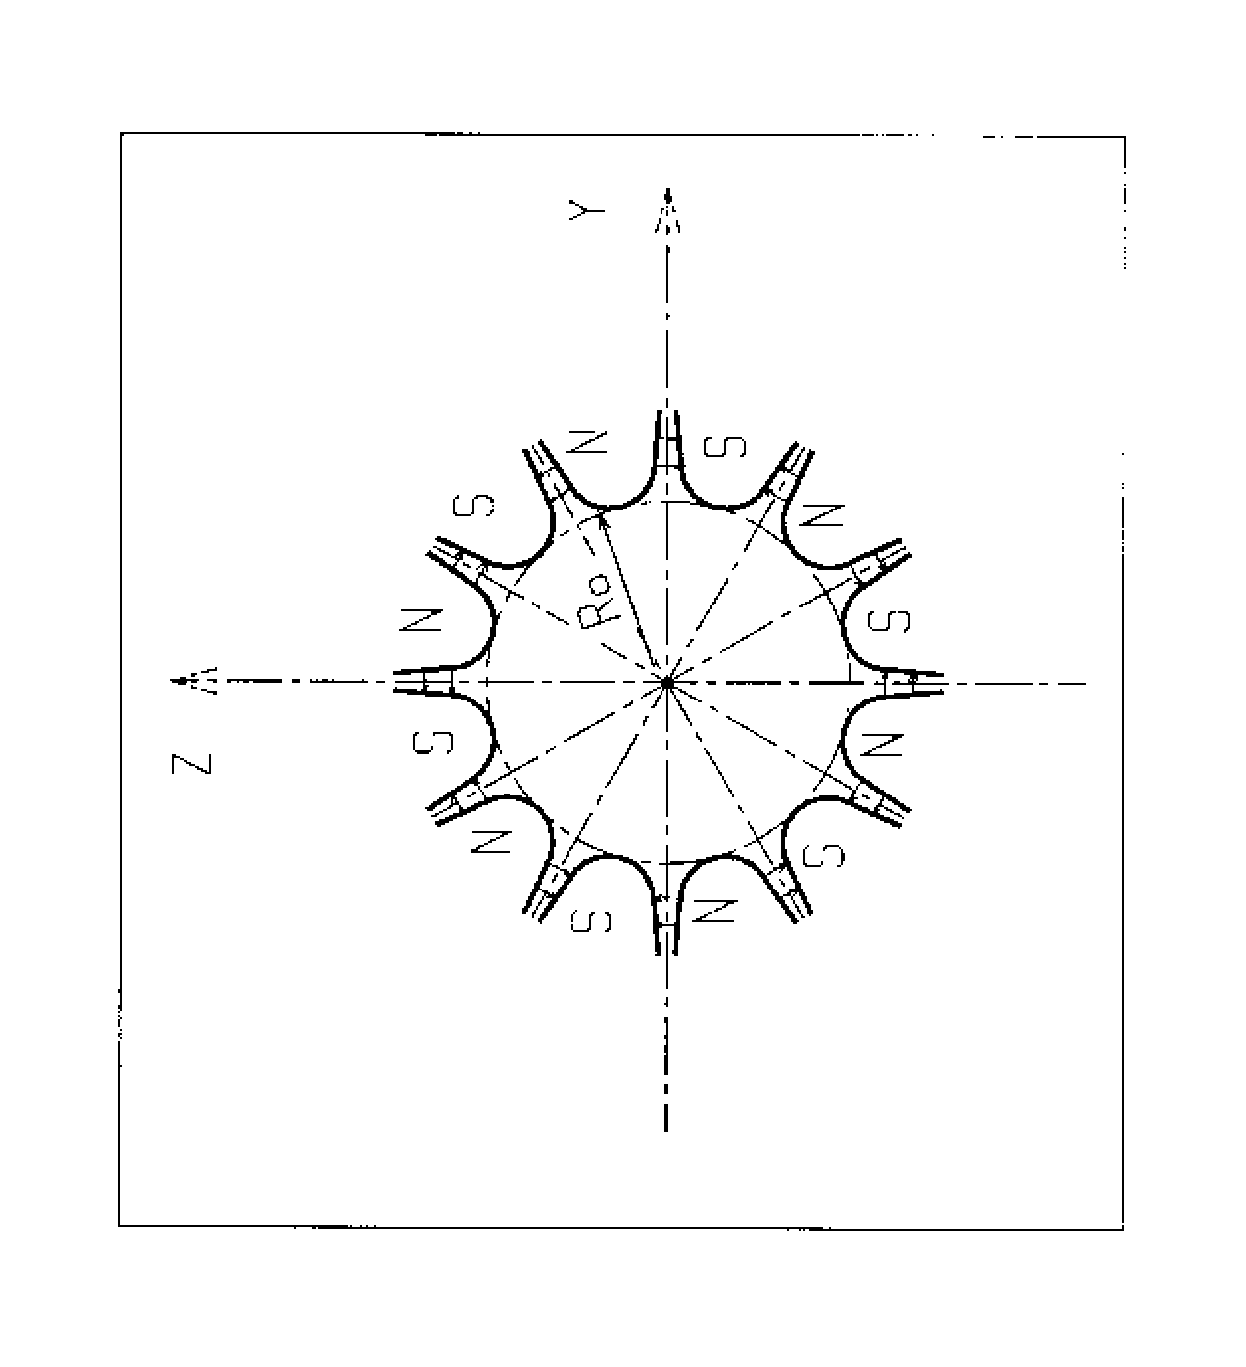
\includegraphics[height=10cm,angle=-90]{Fig19.ps}}
%%%%\hangcaption{\label{fig19}Dodecapole magnet}
\end{figure}
\vfill

\newpage
\begin{tabbing}  %% nouveaux tab
\mestab
\textbf{DRIFT, ESL}         \label{ESL-B} \index{ESL|textbf} \label{DRIFT-B} \index{DRIFT|textbf}
       \> \textbf{\ESLTitl}   \> \> \\
  \\
  \\
 $\XL$         \> length \> cm \> E
 
 \end{tabbing}
 \vfill
 
 %%%%%%%%%%%%%%figure%%%%%%%%%%%%%%
\begin{figure}[H]
%%%Figure 23
\centerline{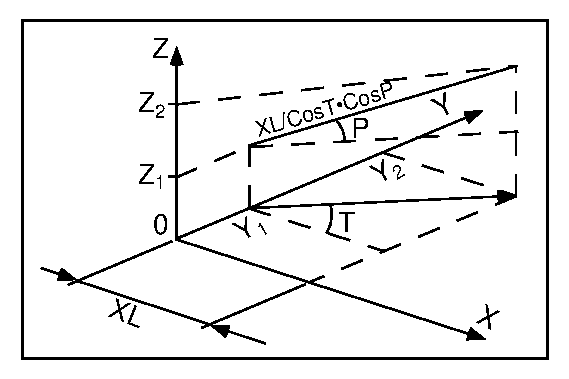
\includegraphics[width=15cm]{Fig23.ps}}
\end{figure}
\vfill

\newpage

\begin{tabbing}
\mestab
\textbf{EBMULT~\footnotemark[1]}         \label{EBMULT-B} \index{EBMULT}
          \> \textbf{\EBMULTTitl} \> \> \\
 \\
 \\
 $\IL$   \>$\IL=1,2[\times 10^n],~7$ : print coordinates, fields, etc., along trajectories \>0-2$[\times 10^n]$, 7 \>I\\
        \> in zgoubi.res ($1$),  zgoubi.plt ($2$),  zgoubi.impdev.out ($7$).       \>                   \> \\
% $\IL$                 \>$\IL=1,2[\times 10^n]$ : print field and coordinates along trajectories. \> 0-2$[\times 10^n]$ \>\\
 \\
 \>\textbf{Electric poles} \>\>\\
 $\XL$, $R_0$, $E1$, $E2$, ..., $E10$  \>Length of element~; radius at pole tip~;
             \>2*cm, 10*V/m \>12*E\\
 \>field at pole tip for dipole, quadrupole, \>\>\\
 \>..., 20-pole electric components \>\>\\
 \\
 \>\textbf{Entrance face} \>\>\\
$ X_E$, $\lambda_ E$, $E_2$, ..., $E_{10}$ 
            \>Integration zone~; fringe field extent : \>2*cm, 9*no dim.\> 11*E\\
 \>dipole fringe field extent = $ \lambda_ E $~; \>\> \\
 \>quadrupole fringe field extent = $ \lambda_ E\ast E_2 $~;\>\>\\
 \>...  \>\>\\
 \>20-pole fringe field extent = $ \lambda_ E\ast E_{10} $ \>\>\\
 \>(for any component : sharp edge if field \>\>\\
 \>extent is zero)\>\>\\
 \\
 \textsl{NCE}, $ C_0-C_5 $            \>same as \textsl{QUADRUPO}  \>0-6, 6*no dim. \>I,6*E\\
 \\
 \>\textbf{Exit face} \>\>\\
$ X_S$, $\lambda_S$, $S_2$, ..., $S_{10} $ \>Integration zone~; as for entrance
           \>2*cm, 9*no dim. \> 11*E\\
 \\
 \textsl{NCS}, $ C_0-C_5 $           \> \> 0-6, 6*no dim. \>I, 6*E \\
 \\
$ R1$, $R2$, $R3$, ..., $R{10}$    \>Skew angles of electric field components \>10*rad \>10*E\\
 \\
 \> \textbf{Magnetic poles} \>\>\\
 $\XL$, $ R_0$, $B1$, $B2$,  ..., $B{10}$
              \>Length of element~; radius at pole tip~; \>2*cm, 10*kG \>12*E\\
 \>field at pole tip for dipole, quadrupole, \>\>\\
 \>..., 20-pole magnetic components \>\>\\
 \\
 \>\textbf{Entrance face} \>\>\\
$ X_E$, $\lambda_E$, $E_2$, ..., $E_{10} $ 
         \>Integration zone~; fringe field extent : \>2*cm, 9*no dim.\> 11*E\\
 \>dipole fringe field extent = $ \lambda_ E $~;\> \> \\
 \>quadrupole fringe field extent = $ \lambda_ E\ast E_2 $~;\>\>\\
 \>...  \>\>\\
 \> 20-pole fringe field extent = $ \lambda_ E\ast E_{10} $ \>\>\\
 \>(for any component : sharp edge if field  \>\>\\
 \>extent is zero)\>\>\\
\\
 \textsl{NCE}, $ C_0-C_5 $            \>same as \textsl{QUADRUPO}  \>0-6, 6*no dim. \>I,6*E\\
\end{tabbing}
\footnotetext[1]{~ Use \textsl{PARTICUL} to declare mass and charge.} 


\newpage %%%


\begin{tabbing}
\mestab
 \>\textbf{Exit face} \>\>\\
$ X_S$, $\lambda_S$, $S_2$, ..., $S_{10} $ \>Integration zone~; as for entrance
           \>2*cm, 9*no dim. \> 11*E\\
 \\
 \textsl{NCS}, $ C_0-C_5 $           \> \> 0-6, 6*no dim. \>I, 6*E \\
 \\
$ R1$, $R2$, $R3$, ..., $R{10}$   
         \>Skew angles of magnetic field components \>10*rad  \>10*E\\
 \\
 \textsl{XPAS}          \>Integration step  \>cm \>E \\
 \\
 \textsl{KPOS}, \textsl{XCE}, \textsl{YCE, ALE}    \>\textsl{KPOS}=1 : element aligned, 2 : misaligned~; shifts, tilt.
           \>1-2, 2*cm, rad \>I, 3*E \\
% \textsl{YCE, ALE}      \>shifts, tilt (unused if \textsl{KPOS}=1)  
\end{tabbing}
\vfill

%%%%%%%%%%%%%%figure%%%%%%%%%%%%%%
\begin{figure}[H]
%\vspace{15 truecm}
%%%Figure 20
\centerline{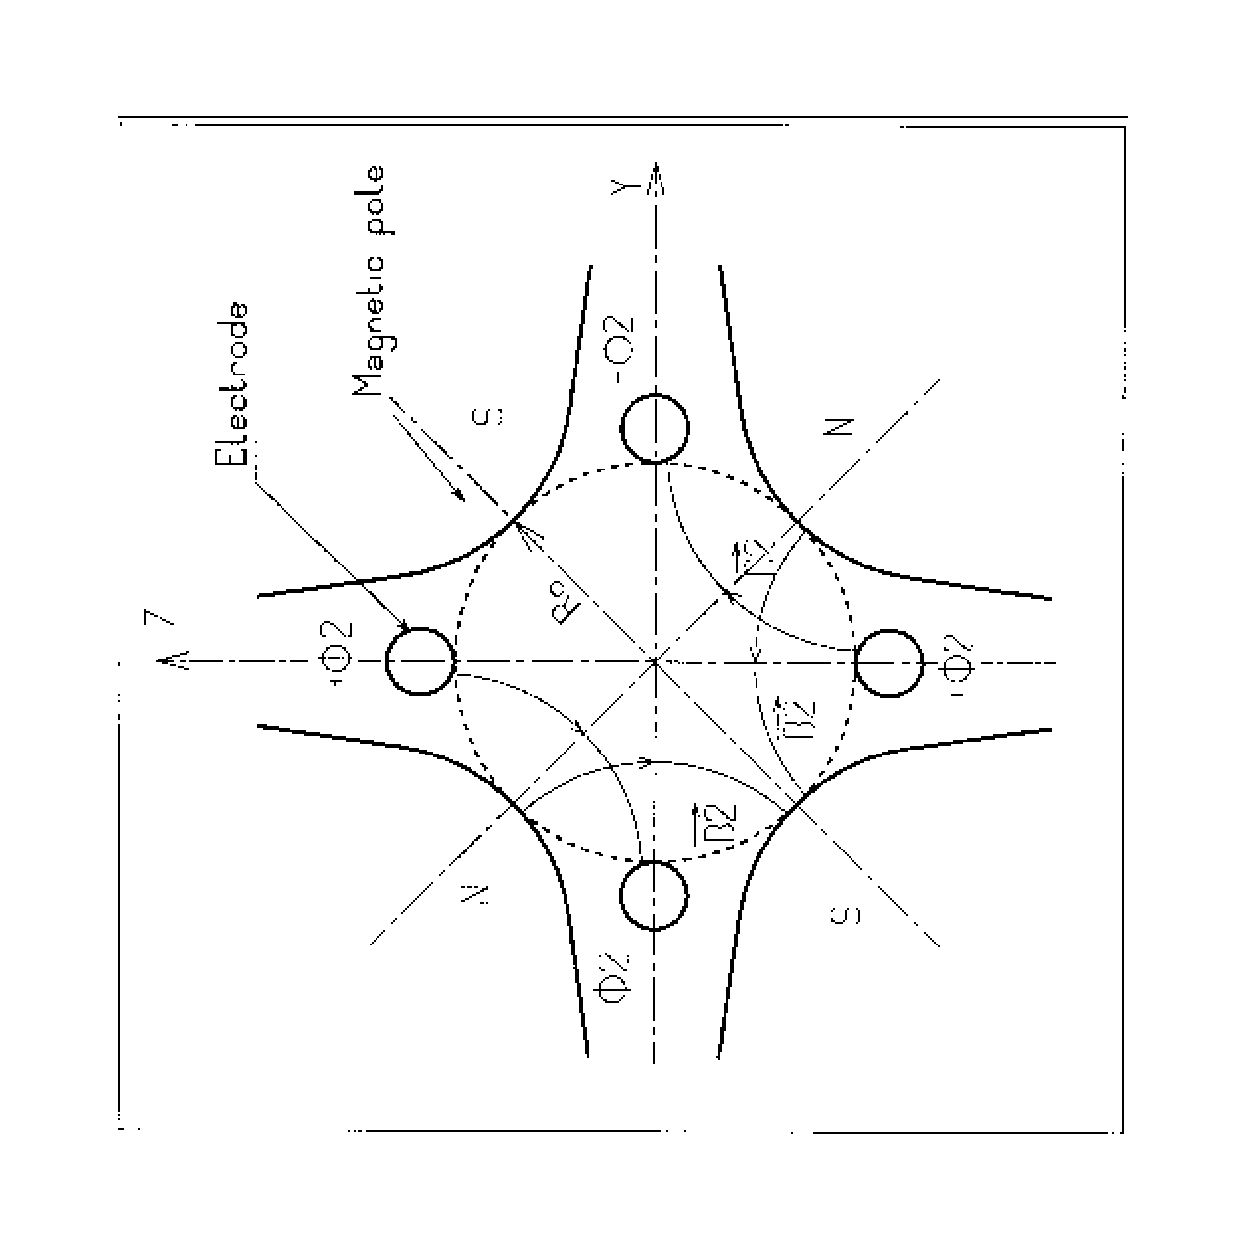
\includegraphics[height=15cm,angle=-90]{Fig20.ps}}
\end{figure}
\vfill

\newpage

\begin{tabbing}
\mestab
\textbf{EL2TUB~\footnotemark[1]}         \label{EL2TUB-B} \index{EL2TUB|textbf}
          \>\textbf{\ELTwoTUBTitl}\ \>\>\\
 \\
 \\
 $\IL$   \>$\IL=1,2[\times 10^n],~7$ : print coordinates, fields, etc., along trajectories \>0-2$[\times 10^n]$, 7 \>I\\
        \> in zgoubi.res ($1$),  zgoubi.plt ($2$),  zgoubi.impdev.out ($7$).       \>                   \> \\
 \\
$ X_1$, $D$, $X_2$, $R_0 $  \>Length of first tube~; distance between tubes~; \>3*m \>4*E\\
 \>length of second tube~; inner radius \>\>\\
 \\
$ V_1$, $V_2 $       \>Potentials \>2*V \>2*E \\
 \\
 \textsl{XPAS}          \>Integration step  \>cm \>E \\
 \\
 \textsl{KPOS}, \textsl{XCE},    \textsl{YCE, ALE}     \>\textsl{KPOS}=1 : element aligned, 2 : misaligned~; shifts, tilt.
           \>1-2, 2*cm,   \>I, 3*E \\
\end{tabbing}

\footnotetext[1]{~ Use \textsl{PARTICUL} to declare mass and charge.} 
\vfill
%%%%%%%%%%%%%%figure%%%%%%%%%%%%%%
\begin{figure}[H]
%%%Figure 22
\centerline{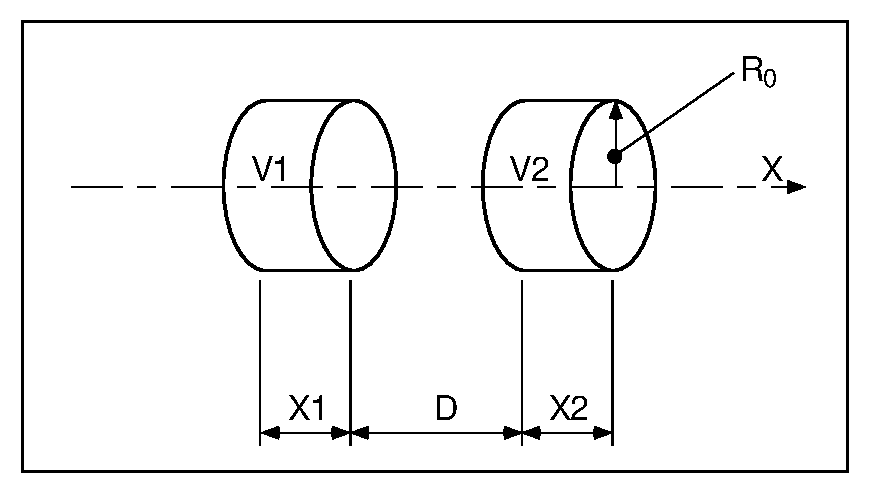
\includegraphics[width=14cm] {Fig22.ps}}
\unnumberedcaption{\CapELtwoTUB}
\end{figure}

\newpage

\begin{tabbing}
\mestab
 \textbf{ELMIR}        \label{ELMIR-B} \index{ELMIR|textbf}
     \> \textbf{\ELMIRTitl} \> \> \\
  \\
\\
 $\IL$   \>$\IL=1,2[\times 10^n],~7$ : print coordinates, fields, etc., along trajectories \>0-2$[\times 10^n]$, 7 \>I\\
        \> in zgoubi.res ($1$),  zgoubi.plt ($2$),  zgoubi.impdev.out ($7$).       \>                   \> \\
%  $\IL$            \>$\IL=1,2[\times 10^n]$ : print field and coordinates along trajectories.  \> 0-2$[\times 10^n]$\> I  \\
  \\
N,$L\!1$, ..., $L\!N$, $D$, \textsl{MT}   \> Number of  electrodes~; electrode lengths~; gap~; \> $2-7$, N*m, m \> I, N*E, E, I \\
  \> mode (11/H-mir, 12/V-mir, 21/V-lens, 22/H-lens)\>  \> \\
\\
$V\!1$, ..., $V\!N$ \> Electrode potentials (normally $V\!1=0$)  \> N*V \> N*E \\
\\
 \textsl{XPAS}          \>Integration step  \>cm \>E \\
 \\
 \textsl{KPOS}, \textsl{XCE},     \>\textsl{KPOS}=1 : element aligned~; 2 : misaligned~; 
           \>1-2, 2*cm, rad \>I, 3*E \\
 \textsl{YCE, ALE}      \>shifts, tilt~; 3 :  automatic  \> \> \\
                        \>   positioning, $YCE=$ pitch, $ALE=$ half-deviation      \> \>
 \end{tabbing}

\vfill
%%%%%%%%%%%%%%figure%%%%%%%%%%%%%%
\begin{figure}[H]
\centerline{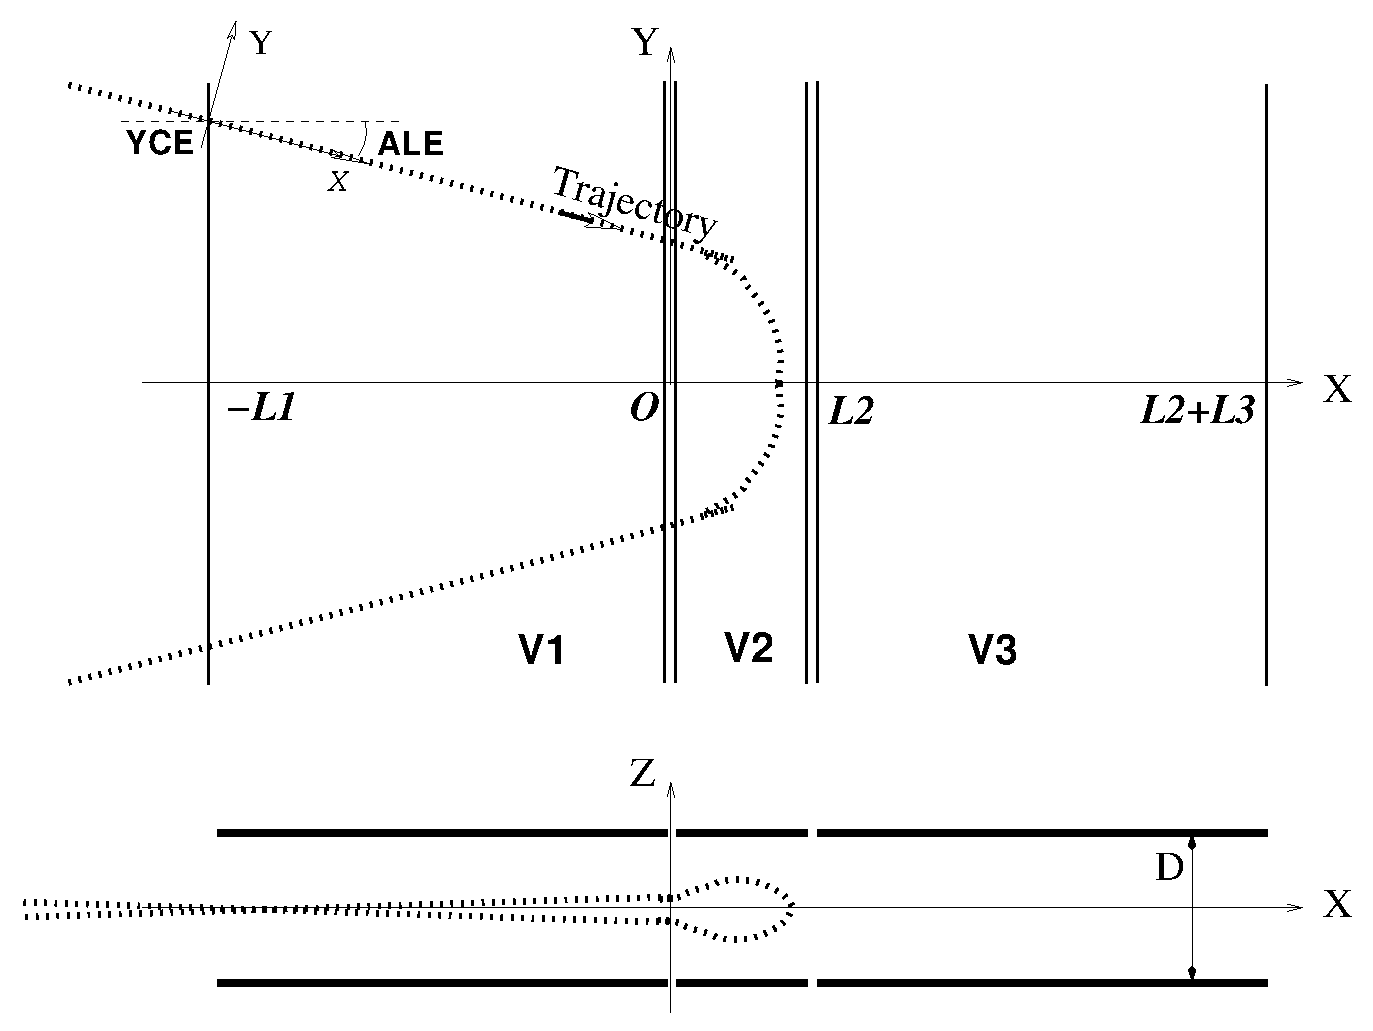
\includegraphics[height=9cm]{FigELMIR.eps}}
% \unnumberedcaption{\CapELMIR} 
\begin{center} \CapELMIR \end{center}
\end{figure}

\vfill 

\newpage

\begin{tabbing}
\mestab
 \textbf{ELMIRC}        \label{ELMIRC-B} \index{ELMIRC|textbf}
     \> \textbf{\ELMIRCTitl} \> \> \\
  \\
\\
 $\IL$   \>$\IL=1,2[\times 10^n],~7$ : print coordinates, fields, etc., along trajectories \>0-2$[\times 10^n]$, 7 \>I\\
        \> in zgoubi.res ($1$),  zgoubi.plt ($2$),  zgoubi.impdev.out ($7$).       \>                   \> \\
%  $\IL$            \>$\IL=1,2[\times 10^n]$ : print field and coordinates along trajectories.  \> 0-2$[\times 10^n]$\> I  \\
  \\
$R1$, $R2$, $A\!T$, $D$ \> Radius of first and second slits~; total deviation \> 4*m \> 4*E \\
  \> angle~; gap \> 2*m, rad, m \> 4*E \\
\\
$V-V\!A$, $V\!B-V$ \> Potential difference \> 2*V \> 2*E \\
\\
 \textsl{XPAS}          \>Integration step  \>cm \>E \\
 \\
 \textsl{KPOS}            \>Normally $KPOS=2$ for positioning~;  \>1-2 \>I\\
 RE, TE, RS, TS     \>Radius and angle at respectively entrance and exit. \>cm, rad, cm, rad \>4*E \\

 \end{tabbing}

\vfill
%%%%%%%%%%%%%%figure%%%%%%%%%%%%%%
\begin{figure}[H]
\centerline{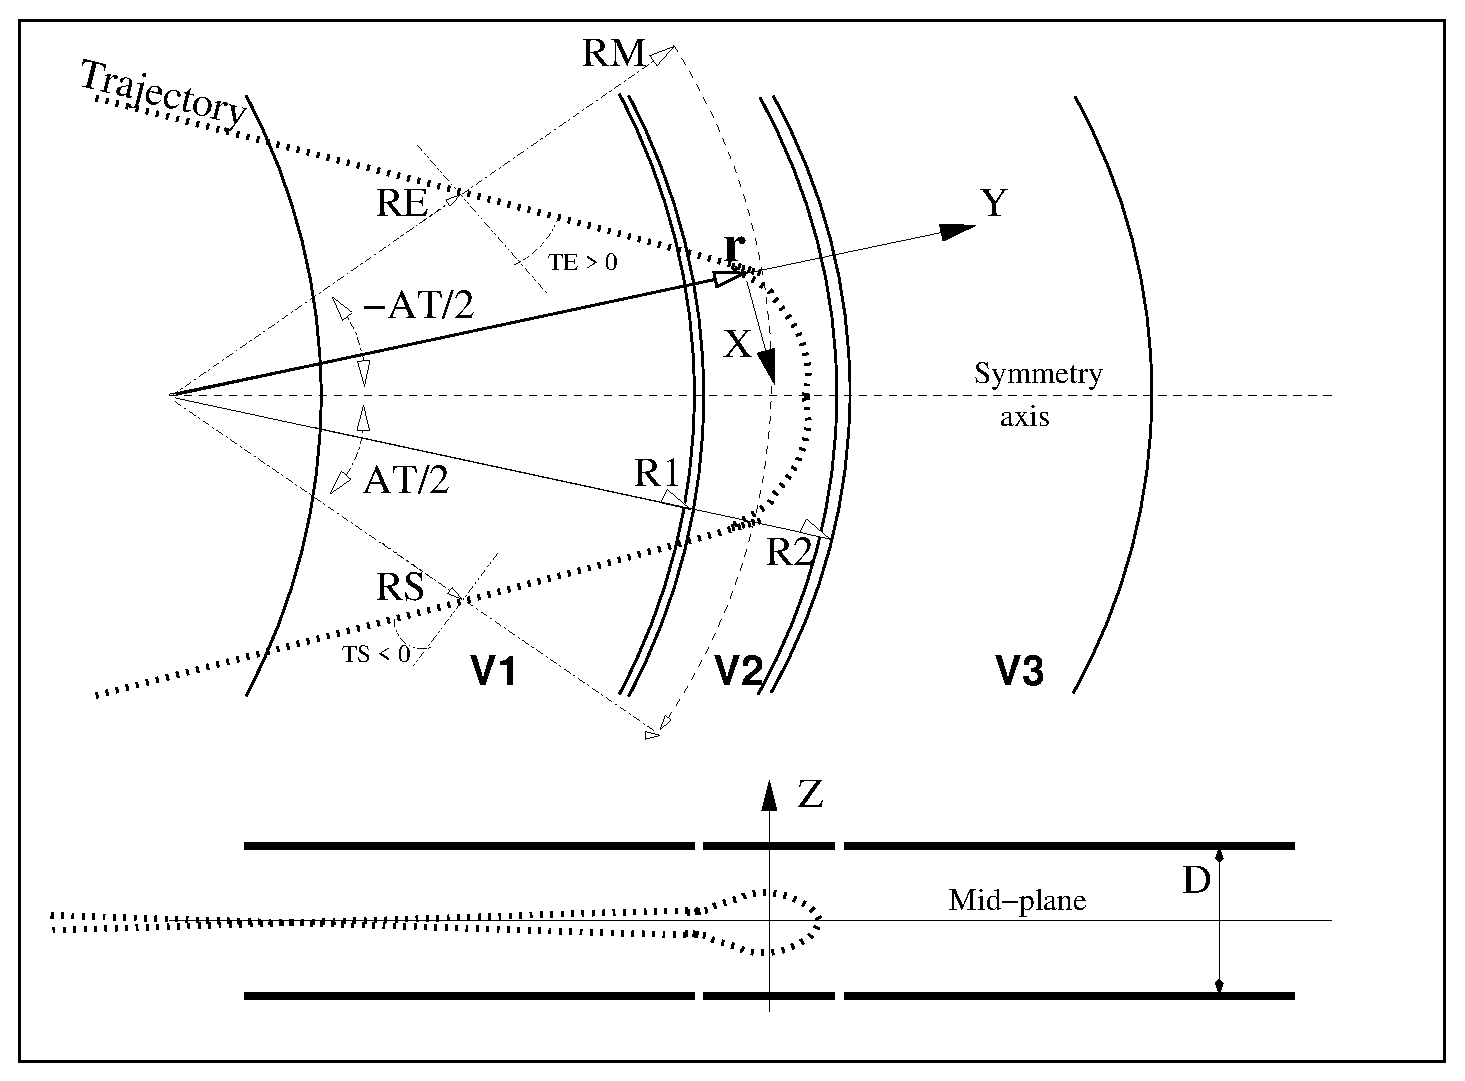
\includegraphics[height=9cm]{FigELMIRC.eps}}
\unnumberedcaption{\CapELMIRC}
\end{figure}

\vfill 

\newpage

\begin{tabbing}
\mestab
\textbf{ELMULT~\footnotemark[1]}         \label{ELMULT-B} \index{ELMULT|textbf}
           \> \textbf{\ELMULTTitl }\> \> \\
 \\
 \\
 $\IL$   \>$\IL=1,2[\times 10^n],~7$ : print coordinates, fields, etc., along trajectories \>0-2$[\times 10^n]$, 7 \>I\\
        \> in zgoubi.res ($1$),  zgoubi.plt ($2$),  zgoubi.impdev.out ($7$).       \>                   \> \\
% $\IL$                 \>$\IL=1,2[\times 10^n]$ : print field and coordinates along trajectories.\>  0-2$[\times 10^n]$ \> I \\ 
 \\
 $\XL$, $R_0$, $E1$, $E2$,  ..., $E{10}$ \>Length of element~; radius at pole tip~;
        \>2*cm, 10*V/m \>12*E\\
 \>field at pole tip for dipole, quadrupole, \>\>\\
 \>..., dodecapole components \>\>\\
 \\
 \>\textbf{Entrance face} \>\>\\
$ X_E$, $\lambda_E$, $E_2$, ..., $E_{10} $ \>Integration zone~; fringe field extent :
\>2*cm, 9*no dim.\> 11*E\\
 \>dipole fringe field extent = $ \lambda_ E $~;\> \> \\
 \>quadrupole fringe field extent = $ \lambda_ E\ast E_2 $~;\>\>\\
 \>... \>\>\\
 \>20-pole fringe field extent = $ \lambda_ E\ast E_{10} $ \>\>\\
 \>(sharp edge if field extent is zero) \>\>\\
 \\
 $NCE$, $ C_0-C_5 $            \>same as \textsl{QUADRUPO}  \>0-6, 6*no dim. \>I, 6*E\\
 \\
 \>\textbf{Exit face} \>\>\\
$ X_S$, $\lambda_S$, $S_2$, ..., $S_{10} $ \>Integration zone~; as for entrance
        \>2*cm, 9*no dim. \> 11*E\\
 \\
 \textsl{NCS}, $ C_0-C_5 $           \> \> 0-6, 6*no dim. \>I, 6*E \\
 \\
$ R1$, $R2$, $R3$, ..., $R{10}$    \>Skew angles of field components \>10*rad \>10*E\\
 \\
 \textsl{XPAS}          \>Integration step  \>cm \>E \\
 \\
 \textsl{KPOS}, \textsl{XCE},    \textsl{YCE, ALE}        \>\textsl{KPOS}=1 : element aligned, 2 : misaligned~; shifts, tilt.
           \>1-2, 2*cm, rad \>I, 3*E \\
\end{tabbing}

\vspace{-1cm}
\footnotetext[1]{~ Use \textsl{PARTICUL} to declare mass and charge.
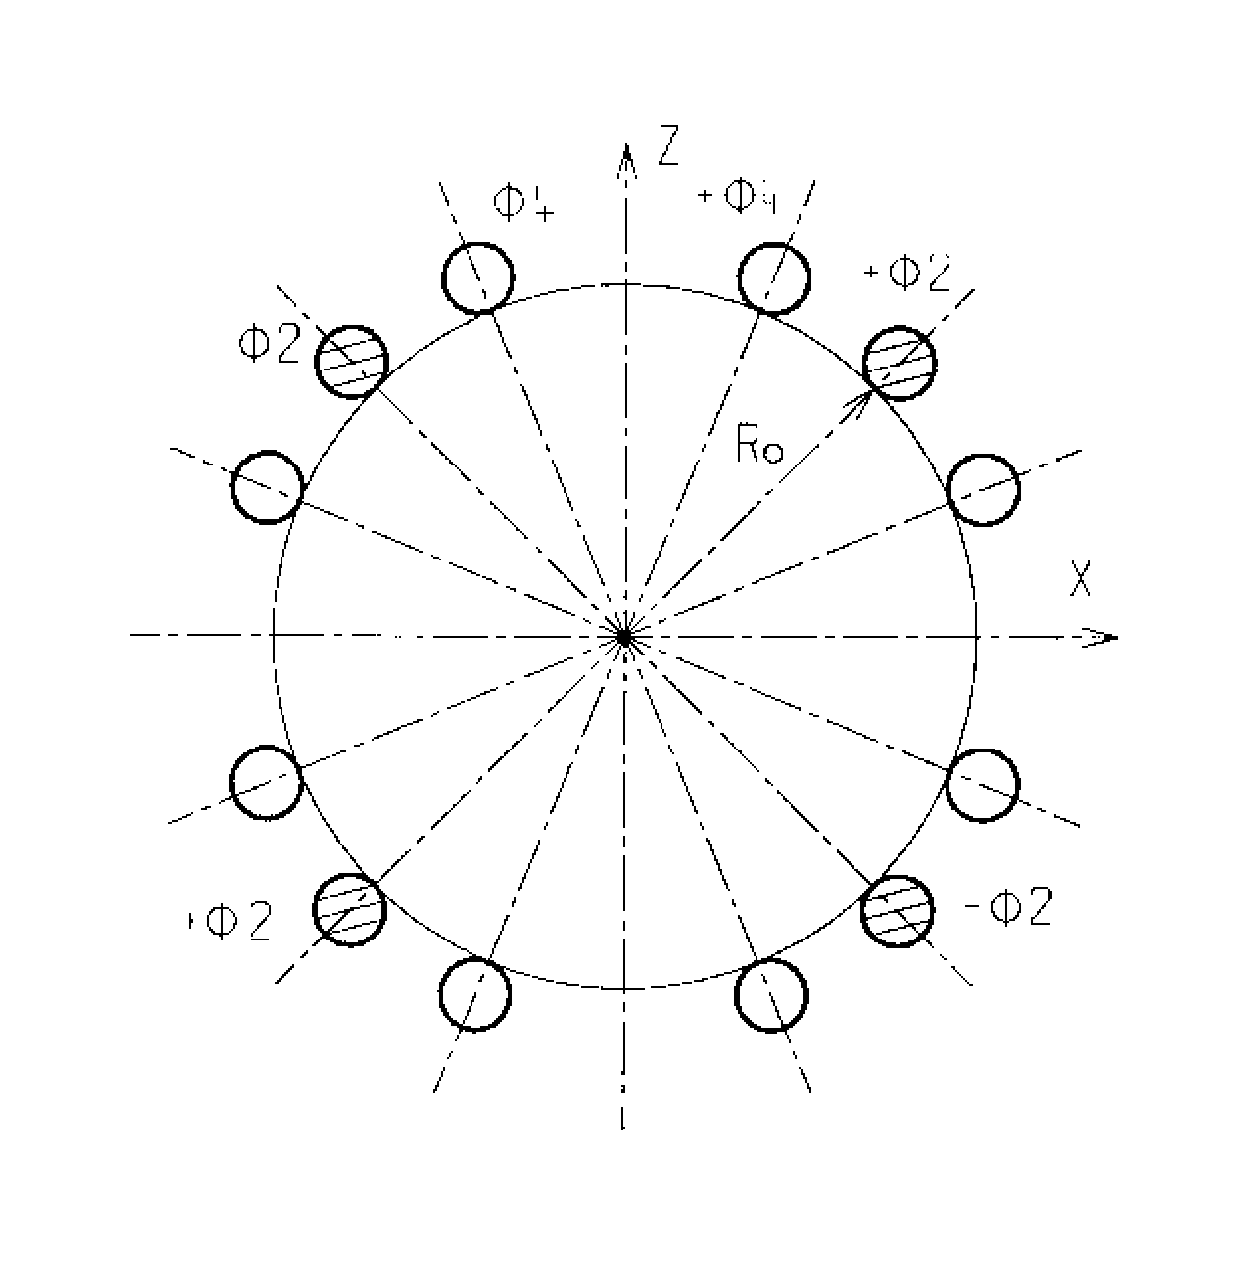
\includegraphics[height=8.5cm]{Fig21bis.ps}} 



\newpage

\begin{tabbing}
\mestab
\textbf{ELREVOL~\footnotemark[1]} \label{ELREVOL-B} \index{ELREVOL|textbf}
         \>\textbf{\ELREVOLTitl  }\> \>    \\
 \>$X$-axis cylindrical symmetry is assumed \>\>\\
 \\
 \\
 $\IC$, $\IL$      \>$\IC=1,2$ : print the map \>0-2; 0-2$[\times 10^n]$, 7 \>2*I\\
   \>$\IL=1,2[\times 10^n],~7$ : print coordinates, fields, etc., along trajectories \> \>   \\
        \> in zgoubi.res ($1$),  zgoubi.plt ($2$),  zgoubi.impdev.out ($7$).       \>                   \> \\
% \>$\IL=1,2[\times 10^n]$ : print field and coordinates along trajectories. \> \> \\
 \\
 \textsl{ENORM, X-NORM}      \> Field and X-coordinate normalization  coeff.  \> 2*UnitConv. \> 2*E \\
        \> Convert values  as read from map file, to MV/cm and cm units. \\
 \\
 \textsl{TITL}        \>Title. Start with ``FLIP'' to get field map X-flipped. \> \>A80 \\
 \\
 $IX$         \>Number of longitudinal nodes of the map \> $\leq$ 400 \>I \\
 \>\>\>\\
 \textsl{FNAME~\footnotemark[2]}    \>File name  \> \>A80 \\
 \\
 $ID$, $A$, $B$, $C$   \>Integration boundary. Ineffective when $ID=0$.      \>$\geq -1$, 2*no dim., \>I,3*E  \\
 {[}, $A'$, $B'$, $C'$,   \>$ID=$ -1, 1 or $\geq 2$ : as for  \textsl{CARTEMES} \> cm {[},2*no dim.,\>[,3*E,etc.]\\
 $B''$, etc., if $\left. ID\geq 2\right]$ \>                                  \> cm, etc.]       \> \\
 \\
 \textsl{IORDRE}     \> Unused \>2, 25 or 4 \>I\\
 \\
 \textsl{XPAS}          \>Integration step  \>cm \>E \\
 \\
 \textsl{KPOS}, \textsl{XCE},     \textsl{YCE, ALE}   \>\textsl{KPOS}=1 : element aligned, 2 : misaligned~; shifts, tilt.
           \>1-2, 2*cm, rad \>I, 3*E \\
\end{tabbing}

\vspace{-2.cm}
\footnotetext[1]{~ Use \textsl{PARTICUL} to declare mass and charge.} 
\begin{alltt}
\footnotetext[2]{ \textrm{\textsl{FNAME} (\emph{e.g.}, e-lens.map) contains the field data. These must be formatted according to the following \textsl{FORTRAN} sequence : }

	      OPEN (UNIT = NL, FILE = FNAME, STATUS = `OLD' [,FORM='UNFORMATTED'])
	      DO 1 I = 1, IX
	         IF (BINARY) THEN 
	            READ(NL) X(I), EX(I)
	         ELSE
	            READ(NL,*) X(I), EX(I)
	         ENDIF 
        1     CONTINUE

 \textrm{where \(X(I)\) and \(EX(I)\) are the longitudinal coordinate and field component at node \((I)\) of the mesh. Binary file names \textsl{FNAME} must begin with  'B\(\sb{_}\)' or 'b\(\sb{_}\)'. `Binary' will then automatically be set to `.TRUE.'}
}\end{alltt} 






\newpage


\begin{tabbing}
\mestab
 \textbf{EMMA}        \label{EMMA-B} \index{EMMA|textbf}
     \> \textbf{\EMMATitl} \> \> \\
 \\
 \\
 $\IL$   \>$\IL=1,2[\times 10^n],~7$ : print coordinates, fields, etc., along trajectories \>0-2$[\times 10^n]$, 7 \>I\\
        \> in zgoubi.res ($1$),  zgoubi.plt ($2$),  zgoubi.impdev.out ($7$).       \>                   \> \\
% $\IC$, $\IL$      \> see \textsl{CARTEMES} \>0-2, 0-2$[\times 10^n]$ \>2*I\\
 \\
 \textsl{BNORM, XN,YN, ZN}      \> Field and  X-,Y-,Z-coordinate normalization coefficients. \> 4*UnitConv. \> 4*E \\
        \> Convert values  as read from map file, to kG and cm or rad. \\
 \\
 \textsl{TITL}        \>Title. Start with ``FLIP'' to get field map X-flipped  \> \>A80 \\
 \\
 $IX$, $IY$, $IZ$, \textsl{MOD[.i]}      \>Number of nodes of the mesh in the $X$, $Y$    \>$\leq 400$, $\leq 200$, \>3*I \\
                              \> and $Z$ directions,  $IZ=1$ for single 2-D map~;     \>  $1$, $\ge 0$[.1-9] \> \\
                              \> \textsl{MOD} : operational and map \textsl{FORMAT} reading mode~\footnotemark[1] \> \> \\
                              \> \textsl{MOD}$\le$19 : Cartesian mesh~; \> \> \\
                              \> \textsl{MOD}$\ge$20 : cylindrical mesh~; \> \> \\
                              \> \textsl{.i}, optional, tells the reading \textsl{FORMAT}, default is '*'. \> \> \\
 \\
\textsl{FNAME}~\footnotemark[1] \>   Names of the $NF$ files that contain the 2-D maps,   \> \>A80 \\
($K=1$, $NF$) \> ordered from $Z(1)$ to $Z(NF)$. \\
      \> If \textsl{MOD}=0 : a single map, superimposition of QF and QD ones, is built for tracking. \\
      \> If \textsl{MOD}=1 : a single map, \textsl{interpolated} from  QF[$x_F$] and QD[$x_D$] ones, is built for tracking. \\
      \> If \textsl{MOD}=22 : a single map, superimposition of QF and QD ones, is built for tracking. \\
      \> If \textsl{MOD}=24 : field at particle is interpolated from a (QF,QD) pair of maps, closest to \\
      \> current $(x_F,x_D)$ value, taken from of set of (QF,QD) pairs registered in FNAME... \\
 \\
 $ID$, $A$, $B$, $C$   \>Integration boundary. Ineffective when $ID=0$.      \>$\geq -1$, 2*no dim., \>I,3*E  \\
 {[}, $A'$, $B'$, $C'$,   \>$ID=$ -1, 1 or $\geq 2$ : as for  \textsl{CARTEMES} \> cm {[},2*no dim.,\>[,3*E,etc.]\\
 $B''$, etc., if $\left. ID\geq 2\right]$ \>                                  \> cm, etc.]       \> \\
 \\
 \textsl{IORDRE}     \>If $IZ=1$ : as in \textsl{CARTEMES\index{CARTEMES}}  \>2, 25 or 4 \>I\\
                     \>If $IZ \not =1$ : unused  \>  \>\\
 \\
 \textsl{XPAS}          \>Integration step  \>cm \>E \\
 \\
 \textsl{KPOS}, \textsl{XCE},  \textsl{YCE, ALE}        \>\textsl{KPOS}=1 : element aligned, 2 : misaligned~; shifts, tilt.  
  \>1-2, 2*cm, rad \>I, 3*E \\
 \end{tabbing}


\footnotetext[1]{~ \textrm{\textsl{FNAME} normally contains  the field map data. If \textsl{MOD}=24 \textsl{FNAME(K)} contains the names of the QF maps and QD maps, as well as the QF-QD distance attached to each one of these pairs.}}




\newpage


\begin{tabbing}
\mestab
~ ~ $ \omega^+$, $\theta$,     $R_1$, $U_1$, $U_2$, $R_2 $ ~ ~ ~  ~ ~    \quad \=
 �$ B=\mathcal{F}B_0 \left(1+N \left(\frac{R-RM }{ RM} \right)      
                +B \left(\frac{R-RM}{ RM} \right)^2+G \left(\frac{R-RM }{ RM}
                \right) \right) $ \quad  \= 2*cm, 2*deg \quad \= \kill
%%%%%%%%%
 \textbf{ERRORS}        \label{ERRORS-B} \index{ERRORS|textbf}
     \> \textbf{\ERRORSTitl} \> \> \\
     \> (UNDER DEVELOPMENT)\\
\\
\\
\textsl{ONF, NBR, SEED [, PRINT]}  \> On/off switch (0/1)~; number of error sets to be injected (\ie,  \> ,,,[,] \> I1, I, I [,A5] \\
                              \> as well, number of lines  following this one)~; random seed. \> \> \\
                              \> Occurence of \textsl{PRINT} will save error series in  \> \> \\
                              \>  zgoubi.ERRORS.out. \> \> \\
 \\
 \textbf{The next line depends on the optical element of concern, and is to be one of the following~: } \\
\textbf{(only limited possibilities at the moment, under development) } \\
\\
 \textsl{MULTIPOL[\{LBL1 [,LBL2]\}]}, 
                        \> Keyword concerned [optionally, first and/or second label]~; \> ,[,],,,,2*kG, \>A8 [,A10[,A10]],  \\
\textsl{N, TYP, AR, UG,}\> N=1-10~: pole  concerned (dipole to 20-pole)~;              \> \>I, A2, A1, \\
\textsl{VC, HW, CUTOFF} \>TYP= BP~: field at pole~; AR=A or R~: field value is absolute \> \> A1, 3*E  \\
                        \> or relative (to current one)~; UG=U or G~: uniform or Gaussian  \> \> \\
                        \> random law~; VC= central value~; HW= half-width (case UG=U)  \\
                        \> or sigma (case UG=G)~; cut-off value in units of sigma (unused  \\
                        \> in uniform case) \\
\\
 \textsl{TOSCA[\{LBL1 [,LBL2]\}]}, 
                        \> Keyword concerned [optionally, first and/or second label]~; \> ,[,],,,,2*kG, \>A8 [,A10[,A10]],  \\
\textsl{N, TYP, AR, UG,}\> N=1~: pole  concerned (dipole)~;              \> \>I, A2, A1, \\
\textsl{VC, HW, CUTOFF} \>TYP= BP~: field~; AR=A or R~: field value is absolute \> \> A1, 3*E  \\
                        \> or relative (to current one)~; UG=U or G~: uniform or Gaussian  \> \> \\
                        \> random law~; VC= central value~; HW= half-width (case UG=U)  \\
                        \> or sigma (case UG=G)~; cut-off value in units of sigma (unused  \\
                        \> in uniform case). \\
                        \> If AR=A : BNORM is chsnged to VC + $\delta B$, \\
                        \> if AR=A : BNORM is chsnged to VC + $\delta B/B$, \\
                        \> with  $\delta B$ uniform (UG=U) or Gaussian (UG=G). \\
\\
\end{tabbing}



\vfill

{\noindent $\bullet$ {\bf \textsl{Example}} 
\\
{\small
\begin{verbatim}
'ERRORS'     
1 1 123456  
MULTIPOL{VKICK}  6     BP A U 0.d0  1.   3  
\end{verbatim}
}
\noindent In this example the various attributes of the error keyword take the following value and meaning~: 

\noindent First line~: 

- \textsl{ONF = 1}, error setting is on, \textsl{NBR=1}, only one line follows (only one set of errors in a single keyword,
 \textsl{seed = 123456}

\noindent second line~: 

- \textsl{MULTIPOL} keywords in zgoubi.dat sequence are concerned, only those \textsl{MULTIPOL} featuring ``\textsl{VKICK}'' as 
first label, 

- multipole component N=6, \ie, dodecapole component, will be modified, as follows

- \textsl{BP, A, U, 0.d0, 1., 3}~: absolute (AR=A) field value (TYP=BP) for that component, will be sorted in a uniform (UG=U) random distribution centered on 0 (VC=0.d0) with half-width 1~kG (HW=1.), CUTOFF=3 here is unused (only used for Gaussian distributions, case UG=G). 













\newpage


\begin{tabbing}
\mestab
~ ~ $ \omega^+$, $\theta$,     $R_1$, $U_1$, $U_2$, $R_2 $     \quad \=
 �$ B=\mathcal{F}B_0 \left(1+N \left(\frac{R-RM }{ RM} \right)      
                +B \left(\frac{R-RM}{ RM} \right)^2+G \left(\frac{R-RM }{ RM}
                \right) \right) $, more \quad  \= 2*cm, 2*deg, cm ~ ~ \quad \= \kill
%%%%%%%%%
\textbf{FAISCEAU}         \label{FAISCEAU-B} \index{FAISCEAU|textbf}
  \> \textbf{\FAISCEAUTitl }   \> \> \\
  \\
  \\
 \> Print particle coordinates at the location where the \\
 \> keyword is introduced in the structure.\\[60pt]
%
%
\textbf{FAISCNL}  \label{FAISCNL-B} \index{FAISCNL|textbf} 
            \> \textbf{Store particle coordinates in file FNAME}   \> \> \\
   \\
   \\
 \textsl{FNAME}$^{ 1}$ 
       \>Name of storage file  \> \>A80 \\
       \>(\emph{e.g.},~zgoubi.fai\index{zgoubi.fai}, or b\_zgoubi.fai for binary storage). \> \> \\[60pt] 
%
%
\textbf{FAISTORE}  \label{FAISTORE-B} \index{FAISTORE|textbf}
          \> \textbf{Store coordinates every $I\!P$ other pass [, at 
          elements with appropriate label]}   \> \> \\
   \\
   \\
 \textsl{FNAME}~~\footnotemark[1] 
       \>Name of storage file (\emph{e.g.}~zgoubi.fai). Optional~: a series of up to 10 label(s),   \> \>A80, \\ %%
{[,}\textsl{\LABEL(s)}{]}  \index{LABEL@{\LABEL}}   \> (the first label of element(s) 
             at the exit of which the store will occur)~; \> \>  [, 0-10*A10] \\ 
     \> wild card accepted, in the form \textsl{'*myLabel'} or \textsl{'myLabel*'}.  \> \> \\
     \> If either \textsl{FNAME} or first \textsl{LABEL} is 'none' then \textsl{FAISTORE} is inhibited.  \> \> \\
     \>  Store occurs at all elements if  first \textsl{LABEL}  is 'all' or 'ALL'. \> \> \\
       \\
 $I\!P$ 	\> Store every $I\!P$ other pass (when using 
 \textsl{REBELOTE}\index{REBELOTE} with \textsl{NPASS}\index{NPASS} $\geq I\!P-1$). \> \> I \\
\end{tabbing}




\footnotetext[1]{~ Stored data can be read back from  \textsl{FNAME} using \textsl{OBJET}, \textsl{KOBJ} = 3.}








\newpage

\begin{tabbing}
\mestab
\textbf{FFAG}         \label{FFAG-B} \index{FFAG magnet, radial|textbf}
           \>\textbf{\FFAGTitl}   \> \>   \\
\> {\bf UNDER DEVELOPMENT}\> \>   \\
 \>$ B_Z= \sum_{i=1}^N \Bz_{0,i} \, \mathcal{F}_i(R,\theta) \, \left(   R/R_{M,i} \right)^{K_i}  $ \> \> \\
 \\
 $\IL$   \>$\IL=1,2[\times 10^n],~7$ : print coordinates, fields, etc., along trajectories \>0-2$[\times 10^n]$, 7 \>I\\
        \> in zgoubi.res ($1$),  zgoubi.plt ($2$),  zgoubi.impdev.out ($7$).       \>                   \> \\
% $\IL$    \>$\IL=1,2[\times 10^n]$ : print field and coordinates along trajectories.\> 0-2$[\times 10^n]$ \>  I  \\
 \\
 $N$, $AT$,  $RM$       \> Number of dipoles in the FFAG $N$-tuple~;  \> no dim.,  \> I, 2*E\\
       \> total angular extent  of the dipole~;  reference radius \> deg, cm \>   \\
 \\
\textsl{ Repeat $N$ times the following sequence} \rule{40mm}{.1mm} \> \> \> \\
 \\
 \textsl{ACN}, $\delta R\!M$,  \> Azimuth for dipole positioning~; $R_{M,i}=R\!M + \delta R\!M$~; 
                                                     \> deg, cm, kG,  \> 4*E \\
 $ \Bz_{0}$, $K$ \>  field at $R_{M,i}$~; index 
                                                     \> no dim. \> \\
 \\
 \>ENTRANCE FIELD BOUNDARY \> \> \\
 \\
$g_0$, $\kappa$               \> Fringe field extent ($g=g_0\,(RM/R)^{\kappa}$)  \> cm, no dim. \>2*E\\
 $NC$, $ C_0-C_5 $, shift     \>Unused~; $ C_0 $ to $ C_5 $ : fringe field coefficients~; EFB shift \>0-6, 6*no dim, cm \>I, 7*E \\
$ \omega^ +$, $\theta$, $R_1$, $U_1$, $U_2$, $R_2 $   \>Azimuth of entrance EFB with respect
         to \textsl{ACN}~; \>2*deg, 4*cm   \>6*E\\
 \>wedge angle of EFB~; radii and linear \> \> \\
 \>extents of EFB (use $\mid  U_{1,2}  \mid  = \infty$ when $R_{1,2}=\infty$)  \>\>\\
 \\
 \>(Note : $ g_0 =0$, $\omega^ + $ = \textsl{ACENT}, $ \theta =0 $ and 
        KIRD=0 for \underbar{sharp edge}) \>\>\\
 \\
 \>EXIT FIELD BOUNDARY (See ENTRANCE FIELD BOUNDARY) \>\>\\
 \\
$g_0$, $\kappa$               \> Fringe field parameters, see above   \> cm, no dim \>2*E\\
 $NC$, $ C_0-C_5 $, shift     \>    \>0-6, 6*no dim, cm \>1, 7*E  \\
$ \omega^-$, $\theta$, $R_1$, $U_1$, $U_2$, $R_2 $   \> \>2*deg, 4*cm \>6*E\\
 \\
 \>(Note : $ g_0 =0$, $\omega^- = -AT+$ \textsl{ACENT}, $ \theta 
 =0 $ and  KIRD=0 for \underbar{sharp edge}) \\
\\
 \>LATERAL FIELD BOUNDARY  {\bf to be implemented - following data not used}  \>\>\\
 \\
$g_0$, $\kappa$               \>    \> cm, no dim \>2*E\\
 $NC$, $ C_0-C_5 $, shift     \>    \>0-6, 6*no dim, cm \>1, 7*E  \\
$ \omega^-$, $\theta$, $R_1$, $U_1$, $U_2$, $R_2 $   \>     \>2*deg, 4*cm \>6*E\\
 \\
\textsl{ End of repeat} \rule{80mm}{.1mm} \> \> \> 
\end{tabbing}


\begin{tabbing}
\mestab
\textsl{KIRD,~Resol}         
 \>  If KIRD=0 :  analytical computation of field derivatives~;  \>0, 2, 25 or 4~; \>I, E\\
 \>   Resol = 2/4 for 2nd/4th order field derivatives computation \>  no dim. \> \\ 
 \>  If KIRD $=2, 4$ or $25$~:  numerical interpolation of field derivatives~; \>  \>\\
 \>  size of flying interpolation mesh is \textsl{XPAS/Resol}  \>  \>\\
 \>  \hspace{10mm} KIRD=2 or 25 : second degree, 9- or 25-point grid \>  \>\\
 \>  \hspace{10mm} KIRD=4 : fourth degree, 25-point grid \>\>\\
 \\
 \textsl{XPAS}            \>Integration step                                 \>cm \>E \\
 \\
 \textsl{KPOS}            \>Positioning of the magnet, normally 2. Two options : \>1-2 \>I\\
 \\
\textbf{If KPOS = 2}     \>Positioning as follows : \>\>\\
 $RE$, $TE$, $RS$, $TS$  \>Radius and angle of reference, respectively, 
               \>cm, rad, cm, rad \>4*E \\
 \>at entrance and exit of the magnet  \\
\textbf{If KPOS = 1}     \>Automatic positioning of the magnet, by means of\>\>\\
 $DP$              \>reference relative momentum \>no dim. \>E \\
\end{tabbing}





\newpage

\begin{tabbing}
\mestab
~ ~ $ \omega^+$, $\theta$,     $R_1$, $U_1$, $U_2$, $R_2 $     \quad \=
 �$ B=\mathcal{F}B_0 \left(1+N \left(\frac{R-RM }{ RM} \right)      
                +B \left(\frac{R-RM}{ RM} \right)^2+G \left(\frac{R-RM }{ RM}
                \right) \right) $, more \quad  \= 2*cm, 2*deg, cm ~ ~ \quad \= \kill
%%%%%%%%%
\textbf{FFAG-SPI}         \label{FFAGSPI-B} \index{FFAG magnet, spiral|textbf}
           \>\textbf{\FFAGSPITitl}   \> \>   \\
\> {\bf UNDER DEVELOPMENT}\> \>   \\
 \>$ B_Z= \sum_{i=1}^N \Bz_{0,i} \, \mathcal{F}_i(R,\theta) \, \left(   R/R_{M,i} \right)^{K_i}  $ \> \> \\
 \\
 $\IL$   \>$\IL=1,2[\times 10^n],~7$ : print coordinates along  trajectories, fields, etc.,  \>0-2$[\times 10^n]$, 7 \>I\\
        \>  into zgoubi.res ($1$) or zgoubi.plt ($2[\times 10^n]$) or  zgoubi.impdev.out ($7$).       \>   \> \\
% $\IL$    \>$\IL=1,2[\times 10^n]$ : print field and coordinates along trajectories.\> 0-2$[\times 10^n]$ \>  I  \\
 \\
 $N$, $AT$,  $RM$       \> Number of dipoles in the FFAG $N$-tuple~;  \> no dim.,  \> I, 2*E\\
       \> total angular extent  of the dipole~;  reference radius. \> deg, cm \>   \\
 \\
\textsl{ Repeat $N$ times the following sequence} \rule{40mm}{.1mm} \> \> \> \\
 \\
 \textsl{ACN}, $\delta R\!M$,  \> Azimuth for dipole positioning~; $R_{M,i}=R\!M + \delta R\!M$~; 
                                                     \> deg, cm, kG,  \> 4*E \\
 $ \Bz_{0}$, $K$ \>  field at $R_{M,i}$~; index. 
                                                     \> no dim. \> \\
 \\
 \>ENTRANCE FIELD BOUNDARY \> \> \\
 \\
$g_0$, $\kappa$               \> Fringe field extent ($g=g_0\,(RM/R)^{\kappa}$)  \> cm, no dim. \>2*E\\
 $NC$, $ C_0-C_5 $, shift     \>Unused~; $ C_0 $ to $ C_5 $ : fringe field coefficients~; EFB shift \>0-6, 6*no dim, cm \>I, 7*E \\
$ \omega^ +$, $\xi$,  4 dummies   \>Azimuth of entrance EFB with respect  to \textsl{ACN}~; \>2*deg, 4*unused   \>6*E\\
 \>spiral angle~; 4$\times$unused. \> \> \\
 \\
 \>EXIT FIELD BOUNDARY (See ENTRANCE FIELD BOUNDARY) \>\>\\
 \\
$g_0$, $\kappa$               \> Fringe field parameters, see above    \> cm, no dim \>2*E\\
 $NC$, $ C_0-C_5 $, shift     \>    \>0-6, 6*no dim, cm \>1, 7*E  \\
$ \omega^ -$, $\xi$,  4 dummies   \>  \>2*deg, 4*unused   \>6*E\\
 \>  \> \> \\
\\
 \>LATERAL FIELD BOUNDARY  {\bf to be implemented - following data not used}  \>\>\\
 \\
$g_0$, $\kappa$               \>    \> cm, no dim \>2*E\\
 $NC$, $ C_0-C_5 $, shift     \>    \>0-6, 6*no dim, cm \>1, 7*E  \\
$ \omega^-$, $\theta$, $R_1$, $U_1$, $U_2$, $R_2 $   \>     \>2*deg, 4*cm \>6*E\\
 \\
\textsl{ End of repeat} \rule{80mm}{.1mm} \> \> \> 
\end{tabbing}


\begin{tabbing}
\mestab
~ ~ $ \omega^+$, $\theta$,     $R_1$, $U_1$, $U_2$, $R_2 $     \quad \=
 �$ B=\mathcal{F}B_0 \left(1+N \left(\frac{R-RM }{ RM} \right)      
                +B \left(\frac{R-RM}{ RM} \right)^2+G \left(\frac{R-RM }{ RM}
                \right) \right) $, more \quad  \= 2*cm, 2*deg, cm ~ ~ \quad \= \kill
%%%%%%%%%
\\
\textbf{Integration boundaries} - next line is  optional, starting with string \texttt{IntLim}~: \>\>\\
 \\[-2ex]
\texttt{IntLim}, $ ID$\index{ID@{\textsl{ID}}|textbf}, $A$, $B$, $C$   \>Integration boundary. Line has to start with '\texttt{IntLim}'.  \>$-1,1,2$; deg; cm;  \>I, 3*E\\
$\left[, A'\right.$, $B'$, $\left. C' \right]$\>$ID=-1$~: integration in the magnet begins at entrance  \>deg [; \textsl{id.}]  \>[,3*E]\\ %
                       \>boundary defined by A, B, C. \>     \>           \\
                       \>$ID=1$~: integration is terminated at exit boundary  defined     \> \> \\
                       \>by A', B', C'.                 \> \> \\
                       \>$ID= 2$~: both entrance and exit  boundaries.        \> \> \\
 \\
\textsl{KIRD,~Resol}         
 \>  If KIRD=0 :  analytical computation of field derivatives~;  \>0, 2, 25 or 4~;  \>I, E\\
 \>   Resol = 2/4 for 2nd/4th order field derivatives computation. \> no dim. \> \\ 
 \>  If KIRD $=2,4$ or $25$~:  numerical interpolation of field derivatives~; \>  \>\\
 \>  size of flying interpolation mesh is \textsl{XPAS/Resol}.  \>  \>\\
 \>  \hspace{10mm} KIRD=2 or 25 : second degree, 9- or 25-point grid \>  \>\\
 \>  \hspace{10mm} KIRD=4 : fourth degree, 25-point grid \>\>\\
 \\
 \textsl{XPAS}            \>Integration step                                 \>cm \>E \\
 \\
 \textsl{KPOS},            \>Positioning of the magnet, has to be 2. As follows~: radius and \>2, 2*(cm, rad) \> I, 4*E \\
 $RE$, $TE$, $RS$, $TS$  \>  angle of reference, respectively,  at entrance and exit of the magnet.  \>  \> 
\end{tabbing}



\newpage

\begin{tabbing}
\mestab
\textbf{FIN, END}       \label{FIN-B} \index{FIN|textbf}   \label{END-B} \index{END|textbf}
   \> \textbf{\FINTitl }   \> \> \\
  \\
  \\
 \> Any information in zgoubi.dat following these keywords will be ignored  
\end{tabbing}



\newpage

\begin{tabbing}
\mestab
~ ~ $ \omega^+$, $\theta$,     $R_1$, $U_1$, $U_2$, $R_2 $     \quad \=
 �$ B=\mathcal{F}B_0 \left(1+N \left(\frac{R-RM }{ RM} \right)      
                +B \left(\frac{R-RM}{ RM} \right)^2+G \left(\frac{R-RM }{ RM}
                \right) \right) $ ~ ~   \= 2*cm, 2*deg, cm \quad \quad \= \kill
 \textbf{FIT, FIT2}        \label{FIT-B} \index{FIT|textbf} \index{FIT2|textbf}  \index{constraint (FIT, FIT2)|textbf} 
\index{variable (FIT, FIT2)|textbf}   
          \> \textbf{\FITTitl} \> \> \\
  \\[-2ex]
 $NV$ \textsl{[, nofinal]} \>NV : Number of physical parameters to be varied~; 'nofinal'  \>$\leq 20$ [, nofinal]\>I [, A7] \\ \index{fit procedure!- variable range|textbf} 
 \textsl{[, noSYSout]}   \>  avoids final run (default is~: final run performed  using \> save [string] \> [, A4 [, A80]] \\  
 \textsl{[, save [, FileName]]} \> fitted values, once fit is done)~;  'noSYSout' inhibits system output  \>  \> \\  
  \> of variable and constraint status, except for  start and end, and   \> \\  
  \>  update of penalty value in between~; 'save' saves fit variables   \>  \> \\  
  \>when fit is completed, either in 'FileName' if specified, or   \>  \> \\  
  \>by default in zgoubi.FITVALS.out.  \>  \> \\  
  \\[-1ex]
\textbf{For I = 1, NV}   \> \it repeat NV times the following sequence \> \> \\
  \\[-2ex]
either :     \>    \>    \> \\
 $\IR$, $\IP$, $\XC$, $\DV$  \>Number of the element in the structure~; \> $\leq${\small MXL}~\footnotemark[1], 
{\small $\leq$MXD}~\footnotemark[1], \>2*I, 2*E\\
 \>number of the physical parameter in the element~;\>$\pm$ {\small MXL.MXD}~\footnotemark[3],  \> \\
 \>coupling switch (off = 0)~; variation range ($\pm$).\> relative \> \\
or :     \>    \>    \> \\
 $\IR$, $\IP$, $\XC$, $[V_{min},V_{max}]$  \>  $V_{min}$, $V_{max}$~: lower and upper limits of the variable. 
                                                                          \> see footnote\footnotemark[4] \>2*I, 3*E\\
  \\[2ex]
$ \NC$ ~ \textsl{[, Penalty~[,ITER]]~\footnotemark[3]} \index{fit procedure!- penalty} \index{fit procedure!- max. number of iterations} 
       \>Number of constraints [, penalty [, max. numb. of iterations]].   \> $\leq 20$ [,$10^{-n}$ [,$>0$]] \> I [, E [, I]] \\
 \\[-2ex]
\textbf{For I = 1, NC}  \> \it repeat NC times the following sequence~: \>\>\\
 \\[-2ex]
 $\IC$, $I$, $J$, $I\!R$, $V$~\footnotemark[4], $WV$,  \>$\IC$, $I$ and $J$  define the type of constraint (see table below)~; 
                 \>0-5, 3*($>$0), \>4*I, 2*E, \\
$N\!P$ ~$[,~ p_i(i=1,NP)]$  \>
$I\!R$ : number of the element after which the constraint applies~; \>current unit,  \>  I, $N\!P*$E \\
 \> $V$ : value~; $W$ : weight (the stronger the lower $WV$)\> 2*no~dim.,  \> \\
 \> $N\!P$ : number of parameters~; if $NP\ge 1$, $p_i(i=1,N\!P)$ :  \> curr.~units  \> \\
 \>  parameter values. \> \\
\end{tabbing}

\vfill

\footnotetext[1]{~  The values for the maximum number of elements (\ie, keywords) that a sequence in \zgou\ can contain, MXL, and for the maximum number of parameters under a keyword, MXD,  are set in the include file \texttt{MXLD.H}. }
\footnotetext[2]{~ Data is of the form ``integer.ijk'' with integer$\le$MXD and i, j, k 1-digit integers and such that ijk$\le$MXD. }
\footnotetext[3]{~  FIT[2] ~ will stop when the sum of the squared residuals gets $<$ \textsl{penalty}, or when the maximum allowed number of iterations is reached. }
\footnotetext[4]{~  $V$ is in current \zgou\ units in the case of particle coordinates (\ie, cm, mrad, $\mu$s, momentum 
relative to BORO) and B field (T). It is in MKSA units (m, rad) in the case of matrix coefficients.}




\newpage



\settowidth{\LL}{\textbf{Beam matrix\ }}  
\hspace{-10ex}
\label{TabFITZlst1}
    {\renewcommand{\arraystretch}{1}
%  \newlength{\LL}
\settowidth{\LL}{\textbf{Beam matrix\ }}  \index{fit procedure!constraint|textbf}
{\footnotesize
%	\begin{center}
\hspace{-15ex}
\label{TabFITZlst1}
    {\renewcommand{\arraystretch}{1}
			\begin{tabular}{|>{\bfseries}p{\LL}|c|c|c|c|c|l|p{\LL}|}
			\hline
			\hline
			 \multirow{3}{\LL}{\textbf{Type of constraint}}
			    & \multicolumn{5}{c|}{\rule{0cm}{5mm} \textbf{Parameters defining the constraints}} & 
                            &\multirow{4}{\LL}{\textbf{Recommended \textsl{[MC]OBJET}, and else }}  \\
			\cline{2-7}
			    & \rule{0cm}{5mm}$\mathbf{\IC}$ 
			    & $\mathbf{I}$ & $\mathbf{J}$ & \textbf{Constraint}  
                            &  \multicolumn{2}{c|}{\textbf{Additional parameter(s)}  } &   \\
         & & & & & \multicolumn{1}{c|}{\NP} & \multicolumn{1}{c|}{ Param. values,} & \\[-.5ex]
         & & & & &  & \multicolumn{1}{c|}{ $\pval_1 - \pval_{N\!P}$} & \\
%         & & & & & \multicolumn{1}{c|}{\NP} & \multicolumn{3}{c|}{  value(s), $\pval_{1 - N\!P}$} & \\
	 \hline
         & & & & & & &   \\
	 \multicolumn{1}{|c|}{\mbox{\textbf{Transported  $\sigma$-matrix}}  } 
%	 & 0& 1 - 6 & 1 - 6 & $\sigma_{I\! J}$~~  ($\sigma_{11}=\beta_Y$, $\sigma_{12}=\sigma_{21}=\alpha_Y$, etc.) 
	         & 0& 1 - 6 & 1 - 6 & $\sigma_{I\! J}$~~  ($\sigma_{11}=\beta_Y$, $\sigma_{21,~12}=\alpha_Y$, etc.) 
	         & & &  \scriptsize  \textsl{OBJET/KOBJ=5.1} \\[-.3ex]
         \multicolumn{1}{|c|}{\mbox{($\sigma(s) = T \sigma(0) \tilde T$)}} & & & & & & &   \\
         & & & & & & &   \\
	 \multicolumn{1}{|c|}{\textbf{Periodic \mbox{$\sigma$-matrix} }} 
	         & 0.N & 1 - 6 & 1 - 6 & $\sigma_{I\! J}$~~  ($\sigma_{11}=\cos\mu_Y + \alpha_Y \sin\mu_Y$, etc.) 
	         & & &  \scriptsize  \textsl{OBJET/KOBJ=5.N} \\
	 \multicolumn{1}{|c|}{ ($\sigma = I \cos \mu + J \sin \mu$)}  & ($N\le 9$) &  7 & any & $\mu_Y/2\pi$ & & &  \\
			\multicolumn{1}{|c|}{ (N=1-9  for  }& & 8 & any & $\mu_Z/2\pi$ & & &   \\
			\multicolumn{1}{|c|}{ {\footnotesize \textsl{MATRIX}}} & &  9 & any & $\cos(\mu_Y)$  & & &  \\
			\multicolumn{1}{|c|}{   block 1-9)     } & & 10 & any & $\cos(\mu_Z)$  & & &   \\
                           & & & & & & &   \\
			\multicolumn{1}{|c|}{\textbf{First order}}  
			    & 1  & $1 - 6$ & $1 - 6$ & Transport coeff. $R_{IJ} $  
	 & & &  \scriptsize  \textsl{OBJET/KOBJ=5} \\
	\multicolumn{1}{|c|}{\textbf{transport coeffs.}} &   & 7 & i & $i\ne 8$~: YY-determinant~; i=8~: YZ-det.  & & &   \\
		\multicolumn{1}{|c|}{\textbf{ }}          &   & 8 & j & $j\ne 7$~: ZZ-determinant~; j=7~: ZY-det.   & & &   \\
                           & & & & & & &   \\
		\multicolumn{1}{|c|}{\textbf{Second order}}  
			    & 2  & $1 - 6$ & 1$1 - 6$6 & Transport coeff.  $T_{I,j,k} $  
	 & & &  \scriptsize  \textsl{OBJET/KOBJ=6} \\
			 \multicolumn{1}{|c|}{\textbf{transport coeffs.}} &  &  &  & $  (j= [J/10] ,k=J-10 [J/10] ) $  & & &  \\
			 \multicolumn{1}{|c|}{\textbf{ }}  &  &  &  &  &  & &   \\
                            & & & & & & &   \\
%
			\multicolumn{1}{|c|}{\textbf{Trajectory}}
			    & 3 & $1 - \IMAX$ & $1 - 7$  & $  F(J,I) $ 
         & & &  \textsl{[MC]OBJET}   \\[0.4ex]
			 \multicolumn{1}{|c|}{\textbf{coordinates}}
			    &   &  $-1$      & $1 - 7$  &   $<\! F(J,i)\! >_{i=I1,I2}$ &  \hspace{-1.5ex} {\large $ \left\{ \right. $} \hspace{-3.ex}  $\begin{array}{l} 0\\[-.8ex] 2 \end{array} $ &  \hspace{-1.5ex} $\begin{array}{l} \\[-.8ex] I_1 \end{array}$     $\begin{array}{l} \\[-.8ex] I_2  \end{array} $  &  \scriptsize $\begin{array}{l} 1 \rightarrow \IMAX\\[-.2ex] 1\! \leq \! I_1 \! \leq \! I_2\! \leq\! \IMAX \end{array} $   \\[0.4ex]
			 \multicolumn{1}{|c|}{  \footnotesize (I = particle  }
			    &   &  $-2$      & $1 - 7$  &   $Sup(|F(J,i)|)_{i=1,\IMAX}$ && &    \\
			 \multicolumn{1}{|c|}{ \footnotesize number; J=1-7 for }
			    &   &  $-3$      & $1 - 7$  &  $Dist\left[ F(J,I)_{i=I1,I2}\right]$ &  3 & $I_1$, $I_2$,  $\Delta I$ &  \scriptsize $1\! \leq \! I_1 \! \leq \! I_2\! \leq\! \IMAX $ \\
			 \multicolumn{1}{|c|}{ \footnotesize D,Y,T,Z,P,S,time) }
			    &   &  $-4$      & $1 - 7$  &   $Dist\left[ PU_i, i=1,N \right]$ &  2 &\scriptsize \textsl{NOEL}$_A$,  \textsl{NOEL}$_B$  & \small PU range   \\[0.4ex]
			\multicolumn{1}{|c|}{ }
			    & 3.1 & $1 - \IMAX$ & $1 - 7$  &$|F(J,I) - FO(J,I)|$  & & &    \\
			\multicolumn{1}{|c|}{\textbf{  }}
			    & 3.2 & $1 - \IMAX$ & $1 - 7$  &$|F(J,I) + FO(J,I)|$  & & &   \\
%			\multicolumn{1}{|c|}{\textbf{  }}
%			    & 3.3 & $1 - \IMAX$ & $1 - 7$  & (min($F(J,I)$)+max($F(J,I)$))/2 & 0 & &   \\
			\multicolumn{1}{|c|}{\textbf{  }}
			    & 3.4 & $1 - \IMAX$ & $1 - 7$  &$|F(J,I) - F(J,K)|$  & 1 &K &  \scriptsize $K \! \leq \! \IMAX$ \\
			\multicolumn{1}{|c|}{\textbf{  }}
			    & 3.5 & $1 - \IMAX$ & $1 - 7$  &$(F(J,I) - F(J,K))/F(J,K)$  & 1 & K &  \scriptsize $K \! \leq \! \IMAX$ \\
                            & & & & & & &   \\
%
			\multicolumn{1}{|c|}{\textbf{Ellipse }} 
	 & 4 & $1 - 6$ & $1 - 6$ & $\sigma_{I\! J}$~~  ($\sigma_{11}=\beta_Y$,  
         & & &  \scriptsize  \textsl{OBJET/{\scriptsize  KOBJ=8}~; } \\
                          \multicolumn{1}{|c|}{\textbf{parameters }} 
         &   &         &         & $\sigma_{12}=\sigma_{21}=\alpha_Y$, etc.)
         & & &  \scriptsize  \textsl{MCOBJET/{\scriptsize  KOBJ=3}} \\
                           & & & & & & &   \\
%
			\multicolumn{1}{|c|}{\textbf{Number of}} 
			    & 5 & $-1$ & any &  $N_{survived}/\IMAX$  
         & & &  \scriptsize  \textsl{OBJET} \\
	 \multicolumn{1}{|c|}{\textbf{particles}} &  & $1 - 3$ & any 
           & $N_{in~\epsilon_{Y,Z,X}}/ N_{survived}$ & 1 & $\epsilon_{Y,Z,X}/ \pi $&  \scriptsize  \textsl{MCOBJET}   \\
	 &  & $4 - 6$ & any  & $N_{in~best~\epsilon_{Y,Z,X,rms}}/ N_{survived}$ &  &  &  \scriptsize  \textsl{MCOBJET}   \\
         & & & & & & &   \\
%
	 \multicolumn{1}{|c|}{\textbf{Coordinates \&}}& 7.1 & $1 - \IMAX$ & $1 - 7$ 
                                                                  & min. ($pr_1=1$) or max. (2)  of $F(J,I)$ & 1 & 1-2   
         &  \textsl{[MC]OBJET}   \\
			\multicolumn{1}{|c|}{\textbf{ fields, across}}
			    & 7.2 & $1 - \IMAX$ & $1 - 7$  & max($F(J,I)$) - min$F(J,I)$) &  & &   \\
			\multicolumn{1}{|c|}{\textbf{optical elements  }}
			    & 7.3 & $1 - \IMAX$ & $1 - 7$  & min$F(J,I)$) + max($F(J,I)$) &  & &   \\[0.5ex]
			\multicolumn{1}{|c|}{ \footnotesize (J=1, 2, 3 for   }
			    & 7.6 & $1 - \IMAX$ & $1 - 3$  & min. ($pr_1=1$) or max. (2) value of $B_J$ & 1 & 1-2 &  \\
			\multicolumn{1}{|c|}{ \footnotesize $B_{X,\ Y,\ Z}$) }
			    & 7.7 & $1 - \IMAX$ & $1 - 3$  & max($B_J$) - min($B_J$) &  & &   \\
			\multicolumn{1}{|c|}{\textbf{  }}
			    & 7.8 & $1 - \IMAX$ & $1 - 3$  & min($B_J$) + max($B_J$) &  & &   \\
			\multicolumn{1}{|c|}{\textbf{  }}
			    & 7.9 & $1 - \IMAX$ & $1 - 3$  & $\int B_J \, ds$ & & &   \\
%
         & & & & & & &   \\
	 \multicolumn{1}{|c|}{\textbf{Spin}}
			    & 10 & $1 - \IMAX$ & $1 - 4$  & $  S_{X,Y,Z}(I), ~ |\vec S(I)| $  
         & & &  \textsl{[MC]OBJET}   \\
			\multicolumn{1}{|c|}{\textbf{  }}
			    & 10.1 & $1 -\IMAX$ & $1 -3$  &$|S_{X,Y,Z}(I) -SO_{X,Y,Z}(I)|$
         & & &  \textsl{+SPNTRK}   \\
                            & & & & & & &   \\
			\hline
			\hline
		\end{tabular}  }
~ ~ ~ \\
~ ~ ~ \\
~ ~ ~ 
%	\end{center}
} %\normalsize

\index{fit procedure!- constraint|textbf}




\newpage


\noindent $\bullet$ \textbf{Combining FIT and REBELOTE}~: An example  \label{ExaFITREBELOTE}} 

\smallskip 

\noindent In the example below, \textsl{FIT} requests that (i) the particle trajectory 
with initial coordinates defined by \textsl{OBJET} 
have identical horizontal coordinates at both ends of the snake 
(this is achieved by varying  $Y_0$, $T_0$ in \textsl{OBJET}),   and that 
(ii) the trajectory across the snake - an helix - be $Y\!$-centered  along the snake axis. 

\medskip

The way this works~: 

\medskip

\noindent \textsl{FIT} is executed a first time for $B\rho_{ref}  = BORO=7205.1782956$~kG.cm,\index{BORO@{\BORO}$\times D_{ref}$} \index{BORORef@$B\rho_{ref}$}
 namely the execution loops between \textsl{OBJET} and \textsl{FIT} 
 until the constraints are best fulfilled.  
Once this is completed, the execution pointer then goes to 
the next instruction in the data list, namely  '\textsl{SPNPRT}', this is discussed below, 
and then points to \textsl{REBELOTE}, which will have the 
effect of sending it back to the begining of zgoubi.dat data list. 
However, prior to that, the ``\textbf{1}'' flag, fourth data in first row in \textsl{REBELOTE}, 
requests a change of, next line,  parameter number \textbf{35} in  element  ``\textbf{OBJET}'' (that is, the 
relative regidity of the particle, $D$).  The list of values follows, namely, 
\{1.3872739973  2.1368296674  4.8261190694  11.015241321\}. The change occurs  \textbf{4} times, according to  
\textsl{NRBLT=4}, the first data in  \textsl{REBELOTE} data list. \\
Note that, (i)~spin data so computed (spin 
vector components, precession, etc) are stored/stacked in zgoubi.SPNPRT.Out \index{zgoubi.SPNPRT.Out} 
by placing the keyword '\textsl{SPNPRT}' with label ``\textsl{PRINT}'', between  \textsl{FIT} and  \textsl{REBELOTE}~; 
(ii)~current updated FIT variables are saved in zgoubi.FITVALS.out using the '\textsl{save}' command 
in \textsl{FIT}, and further stacked in zgoubi.FITVALS.out\_cat for each \textsl{REBELOTE} case, using \textsl{SYSTEM}.  

~

\begin{minipage}[h]{.55\linewidth}
{\footnotesize
\begin{verbatim}
Centering 5 helical orbits in the AGS warm helical snake 3-D OPERA map.  
 'OBJET'            ! This data list may be copy-pasted and run, as is.    
7.2051782956D3      ! Reference rigidity of the problem             
2                         
1 1                 ! A single particle. Initial coordinates :      
-2.2  0. 0. 0. 0.  1. 'o'           ! Yo, To, Zo, Po, So, p/po      
1                         
 'PARTICUL'         ! proton data are necessary for spin tracking          
938.27203 1.602176487E-19 1.7928474 0 0     ! M, Q, G factor        
 'SPNTRK'                        
4.1                 ! Initial spin is positionned vertical          
0. 0. 1.                  
                          
 'FAISCEAU'                      
 'SPNPRT'                        
                          
 'TOSCA'                         
0  20                     
1.e1   100. 100. 100.     
HEADER_0 wsnake           
801 29 29 12.1      ! The map is a 801x29x29 node 3-D mesh          
warmSnake.map       ! AGS warm snake 3-D OPERA map                  
0 0 0 0                   
2                         
.1                        
2  0.  .0  0.  0.         
                          
 'FAISCEAU'                      
                          
 'FIT'                           
2   save            ! Two variables. Save FIT variables (in zgoubi.FITVALS.out).  
1 30 0  [-3,3]          ! Vary initial coordinate Y_0 (horiz. position)      
1 31 0  [-3,3]          ! Vary initial coordinate T_0 (horiz. angle)
3    1E-2           ! Three constraints (penalty 2E-3 requested) :  
3.1 1 2 6 0. 1. 0       ! Y_0=Y after at exit of the magnet         
3.1 1 3 6 0. 1. 0       ! T_0=T after at exit of the magnet         
7.3 1 2 6 0. 1. 0       ! Y_min+Y_max=0 inside the OPERA field map  
                          
 'SPNPRT'  PRINT    ! Stack spin data (in zgoubi.SPNPRT.Out).              
 'SYSTEM'           ! Save zgoubi.FITVALS.out data following from successive REBELOTE. 
1                         
cat zgoubi.FITVALS.out >> zgoubi.FITVALS.out_cat                    
                          
 'REBELOTE'         ! Will loop on re-doing the FIT for 4 additional particle rigidities
4  0.1  0 1               
1                   ! List of 4 successive values of D in OBJET follows   
OBJET  35  1.3872739973  2.1368296674  4.8261190694  11.015241321   
                          
 'SYSTEM'           ! Save a copy of zgoubi.FITVALS.out_cat and of zgoubi.SPNPRT.Out_cat
2                         
\cp zgoubi.FITVALS.out_cat zgoubi.FITVALS.out_cat_copy              
\cp zgoubi.SPNPRT.Out      zgoubi.SPNPRT.Out_copy                   
 'END'                                        
\end{verbatim}
\index{zgoubi.SPNPRT.Out}
}
\end{minipage}\hspace{0.03\linewidth}
\begin{minipage}[h]{.37\linewidth}

\centering


\label{FigHelix} 
\centerline{\includegraphics*[bbllx=20,bblly=105,bburx=567,bbury=470,width=.9\linewidth]{Fig-YZ_pwsnk_5.eps}}
%/home/meot/zgoubi/struct/bnl/ags/snakeFieldMaps/rotationAngle/proton/warmSnake/usingTOSCA-3D

This figure shows how, using \textsl{REBELOTE}, 
 the helical trajectories at five different momenta are moved by the \textsl{FIT} procedure, 
one after the other, 
from  initial off-centered position  to final centering on the snake axis (at Y=Z=0). 

\vspace{30ex}

~

\end{minipage}


\newpage

\noindent  $\bullet$  \textbf{FIT[2] options}~: An example \label{FITOptionsExa}  \\

\smallskip 

\noindent \textsl{FIT[2]} options, ``nofinal'', ``save {FileName}'', ``penalty'' and ``ITER'', are 
all specified in the example below. 

~

\begin{minipage}[h]{.55\linewidth}
{\footnotesize
\begin{verbatim}
An example with FIT options
'GETFITVAL'
zgoubi.FITVALS.In
 'MCOBJET'1
57.36635309d3         ! reference rigidity 
3.1                       
1                         
2 2 2 2 1 1               
0. 0. 0. 0. 0.   4.61943880E-01  
 2.703371  1.859656  1.48563786487e-99   9 
-2.592712  2.421706  1.48563786487e-99   9                          
0. 1.  0.     9           
12345 23456 34567 
 'PARTICUL'                                                                                    2
0.51099892 1.60217653e-19 1.15965218076e-3 0.0 0.0                                                            
'PICKUPS'   
  2
 #StartRing MULT BD2S #EndRing
...
 'DRIFT'    DRIF      HD                                                                    7497
14.38218115                                                                                                   
 'MARKER'  #SSMid                                                                           7498
 'MARKER'  #EndRing                                                                         7500
 'FIT2' 
4 save zgoubiFIT.result nofinal  ! Variables saved in zgoubiFIT.result when FIT2 done. No final run.
!!! 4 save nofinal  ! Would cause variables to be saved in default file zgoubi.FITVALS.out instead. 
2 40 0 [-1.e-2,1.e-2]              ! The four variables are Yo, To, Zo, Po in MCOBJET    
2 41 0 [-1.e-2,1.e-2]                      
2 42 0 [-1.e-2,1.e-2]    
2 43 0 [-1.e-2,1.e-2]                      
4   1e-10   90                 ! penalty=1e-10. Maximum allowed calls to zgoubi is 90.
3.1 1 2 7500 0. 1. 0           ! The four constraints are : initial Y, T, Z, P of 
3.1 1 3 7500 0. 1. 0           ! particle #1 equal to its final Y, T, Z, P.           
3.1 1 4 7500 0. 1. 0                                      
3.1 1 5 7500 0. 1. 0                                     
\end{verbatim}
}
\end{minipage}






\newpage

\begin{tabbing}
\mestab
~ ~ $ \omega^+$, $\theta$,     $R_1$, $U_1$, $U_2$, $R_2 $     \quad \=
 �$ B=\mathcal{F}B_0 \left(1+N \left(\frac{R-RM }{ RM} \right)      
                +B \left(\frac{R-RM}{ RM} \right)^2+G \left(\frac{R-RM }{ RM}
                \right) \right) $, more \quad  \= 2*cm, 2*deg, cm ~ ~ \quad \= \kill
\textbf{FOCALE}         \label{FOCALE-B} \index{FOCALE|textbf}
        \> \textbf{\FOCALETitl }\>\>\\
 \\
 \\
 $\XL$      \>Distance from the location of the keyword \> cm \> E \\[60pt] 
\textbf{FOCALEZ}    \label{FOCALEZ-B} \index{FOCALEZ|textbf} 
  \> \textbf{Particle coordinates and vertical beam size at distance \XL} \>\>\\
 \\
 \\
 $\XL$         \>Distance from the location of the keyword \> cm \> E  
\end{tabbing}


\newpage

\begin{tabbing}
\mestab
\textbf{GASCAT}         \label{GASCAT-B} \index{GASCAT|textbf}
        \> \textbf{\GASCATTitl}\>\>\\
 \\
 \\
 $KGA$      \> Off/On switch \> 0, 1 \> I\\
 \\
 $AI$, $DEN$ \> Atomic number~; density\> \> 2*E
 \end{tabbing}
 


\newpage

\begin{tabbing}
\mestab
\textbf{GETFITVAL}         \label{GETFITVAL-B} \index{GETFITVAL|textbf}
        \> \textbf{\GETFITVALTitl}\>\>\\
 \\
 \\
 \textsl{FNAME}      \> Name of storage file. Zgoubi will proceed silently if  \>  \>  A \\
                     \> FNAME='none' or FNAME='NONE', or if the file is not foumd. \>  \>   \\
 \end{tabbing}




\newpage

\begin{tabbing}
\mestab
\textbf{GOTO}         \label{GOTO-B} \index{GOTO|textbf}          \> \textbf{\GOTOTitl} \\[10pt]
%
     \>  \textbf{Under development} \\ %%
%
\\[10pt]
  OPTION     \> Can be 'PASS\#' or 'GOBACK'  \> String \> A \\ %%
\\
\textbf{If OPTION = PASS\#} \> One line needed : \\
\textsl{ LABEL\_1, ..., LABEL\_N}    \> List of labels (expected is label \#1 that follows a keyword) to go to,  \> N strings \> N*A  \\ %%
     \> pass after pass (passes are incremented, from 1 to N, by \textsl{REBELOTE}..\>  %%
\end{tabbing}




\vspace{2ex}
\centerline{\rule{5cm}{0.1mm}}
\vspace{2ex}


\noindent  $\bullet$  Using \textbf{GOTO}~: An example is given page~\pageref{ExaINCLUDE-GOTO} 


 
 \newpage

\begin{tabbing}
\mestab
\textbf{HISTO}  \label{HISTO-B} \index{HISTO|textbf}  \> 
\textbf{\HISTOTitl} \> \> \\
  \\
  \\
$ J$, $X_{\text{min}}$, $X_{\text{max}}$,  \>$J$ = type of coordinate to be histogrammed~; 
             \>1-24, 2*  \>I, 2*E, 2*I\\
\textsl{NBK}, $\NH $     \>the following are available : \>current units,\>\\
 \> $\bullet$ current coordinates :\>$<120$, 1-5 \> \\
 \>\ \ $1(D)$, $2(Y)$, $3(T)$, $4(Z)$, $5(P)$, $6(S)$,\>\> \\
 \>$\bullet$ initial coordinates : \> \> \\
 \>\ \ $11(D_0)$, $12(Y_0)$, $13(T_0)$, $14(Z_0)$, $15(P_0)$, $16(S_0)$,\>\>\\
 \>$\bullet$ spin\index{spin tracking} : \>\>\\
 \>\ \ $ 21(S_X)$, $22(S_Y)$, $23(S_Z)$, $24(<S>)$~;  \>\>\\
 \>$X_{\text{min}}$, $X_{\text{max}}= $ limits of the histogram, in units \>\>\\
 \>of the coordinate of concern~; \textsl{NBK} = number of \>\>\\
 \>channels~; $\NH$ = number of the histogram (for \>\>\\
 \>independence of histograms of the same coordinate) \>\>\\
 \\
 \textsl{NBL, KAR,}    \>Number of lines (= vertical amplitude)~; 
              \>normally 10-40, \>I, A1, I, A1\\
 \textsl{NORM, TYP}    \>alphanumeric character~; normalization if \>char., 
 1-2, P-S-Q \> \\
 \>\textsl{NORM} = 1, otherwise \textsl{NORM} = 0~; \textsl{TYP} = `P' : \>\> \\
 \>primary particles are histogrammed, or `S' : \>\>\\
 \>secondary, or Q : all particles - for use \>\>\\
 \>with \textsl{MCDESINT}  
\end{tabbing}


\newpage

\begin{tabbing}
\mestab
\textbf{IMAGE}         \label{IMAGE-B} \index{IMAGE|textbf} 
         \> \textbf{\IMAGETitl} \\[60pt]
%
\textbf{IMAGES}   \label{IMAGES-B} \index{IMAGES|textbf}
         \> \textbf{Localization and size of horizontal waists} \> \> \\
 \\
 \> For each momentum group, as classified by \> \> \\
 \> means of \textsl{OBJET}, \textsl{KOBJ} = 1, 2 or 4 \\[60pt]
%
\textbf{IMAGESZ}   \label{IMAGESZ-B} \index{IMAGESZ|textbf} 
          \> \textbf{Localization and size of vertical waists} \> \> \\
 \\
 \> For each momentum group, as classified by \> \> \\
 \> means of \textsl{OBJET}, \textsl{KOBJ} = 1, 2 or 4   \\[60pt]
%
\textbf{IMAGEZ}   \label{IMAGEZ-B} \index{IMAGEZ|textbf} 
             \> \textbf{Localization and size of vertical waist} 
\end{tabbing}





\newpage

\begin{tabbing}
~ ~ $ \omega^+$, $\theta$,     $R_1$, $U_1$, $U_2$, $R_2 $    ~ ~ ~ ~ ~  \quad \=
 �$ B=\mathcal{F}B_0 \left(1+N       
                +B \left(\frac{R-RM}{ RM} \right)^2+G \left( ~ 
                \right) \right) $, more ~ ~ ~ \quad  \= 2*cm \quad \= \kill
%\mestab
\textbf{INCLUDE}         \label{INCLUDE-B} \index{INCLUDE|textbf} 
         \> \textbf{\INCLUDETitl} \\[10pt]
%
\\
 \textsl{NBF}       \>Number of files to be included.   \> - \>  I \\ %%
\\
\textbf{NBF following lines (one file name per line)~:} \\
\\
 \textsl{FNAME} \textsl{, [ [LBL\_1A [, LBL\_2A]]:}  \>Name of input zgoubi.dat-style file to be included. \textsl{LBL\_A}~:   \> \>A80 [,[A10], [A10]] \\ %
\textsl{[LBL\_1B [, LBL\_2B]]:}   \>  entrance branching tag, \textsl{LBL\_B}~: exit branching tag.  \\ %%
\end{tabbing}


\vspace{2ex}
\centerline{\rule{5cm}{0.1mm}}
\vspace{2ex}

\noindent  $\bullet$  Using \textbf{INCLUDE}~: An example. \label{ExaINCLUDE-GOTO} \\

\smallskip 

\noindent In this example of an energy-recovery electron recirculator, the linac, spreader and combiner data lists 
are given in separate files, declared as  \textsl{INCLUDE}s (see example page~\pageref{ExaREBELOTE} 
for details regarding this recirculator configuration). Using  \textsl{INCLUDE} has a series of  merits~: 

-  it shortens the parent input data file, so making the optical structure more apparent, 

- it allows picking optical spreader, combiner and ring sequences from  files that may actually be 
set to -~for instance~- compute optical parameters~; in that case, LBL\_A and LBL\_B are used for this targetted picking~: they define the ends 
of the sequence to be \textsl{INCLUDE}'d, ignoring the upper and lower parts in the \textsl{INCLUDE}'d file 
(which are specific -~for instance~-  to MATRIX computations).   


\noindent The juggling between the linac, spreaders, combiners and recirculating ring, 
is handled using \textsl{GOTO} statement. 

\bigskip

\begin{minipage}[h]{.55\linewidth}
{\tiny
\begin{verbatim}
eRHIC ENERGY RECOVERY LINAC RECIRCULATOR WITH FFAG ARCS.
 'MCOBJET'                                               1
57.36635309d3         reference rigidity (kG.cm) 
3   
2000
2 2 2 2 1 1    
-5.360667E-03   5.059706E-3  0. 0. 0.   4.619439E-01  'o'
0. 1   0.   3  
0. 1   0.   3  
0. 1.  0.     3
123456 234567 345678                                         
 'PARTICUL'                                              2
0.51099892 1.60217653e-19 1.15965218076e-3 0.0 0.0       
 'SPNTRK'                                                3
 'FAISCEAU'                                              4    
 'SRLOSS'                                                5
1   srLoss     
MULTIPOL       
1  123456      
 'SCALING'                                               6
1  1
MULTIPOL       
-1  
57.36635309 57.36635309                                  
1           11     
 'MARKER'   ARC#S_1                                      7
 'OPTIONS'                                               8
1  1
WRITE OFF                                                
 'MARKER'   MARK      CELLSTART                          9
 'DRIFT'    DRIF      HD                                10
14.547181      
 'MULTIPOL' RBEN      BD2                               11
0  .Dip        
90. 10. 0. -0.87159105   0. 0. 0. 0. 0. 0. 0. 0.
0. 0. 10.00  4.0  0.800 0.00 0.00 0.00 0.00 0. 0. 0. 0.  
4  .1455   2.2670  -.6395  1.1558  0. 0.  0.             
0. 0. 10.00  4.0  0.800 0.00 0.00 0.00 0.00 0. 0. 0. 0.  
4  .1455   2.2670  -.6395  1.1558  0. 0.  0.             
0. 0. 0. 0. 0. 0. 0. 0. 0. 0.                            
#30|90|30    Dip  BD2                                    
3   0.0E+00   4.0704703E-01  -1.5071892929E-03         
 'DRIFT'    DRIF      D                                 12
29.094362      
\end{verbatim}
\index{zgoubi.SPNPRT.Out}
}
\end{minipage}\hspace{0.03\linewidth}
\begin{minipage}[h]{.38\linewidth}
\centering
%\centerline{\includegraphics*[bbllx=20,bblly=100,bburx=567,bbury=470,width=.9\linewidth]{}}
{\tiny
\begin{verbatim}
 'MULTIPOL' RBEN      QF2                               13
0  .Dip        
110.  10.  0. 0.86286642  0. 0.0 0.0 0.0 0.0 0.0 0.0 0.0     
0. 0. 10.00  4.0  0.800 0.00 0.00 0.00 0.00 0. 0. 0. 0.  
4  .1455   2.2670  -.6395  1.1558  0. 0.  0.             
0. 0. 10.00  4.0  0.800 0.00 0.00 0.00 0.00 0. 0. 0. 0.  
4  .1455   2.2670  -.6395  1.1558  0. 0.  0.             
0. 0. 0. 0. 0. 0. 0. 0. 0. 0.                            
#30|110|30    Dip  QF2                                   
3   0.  -3.6008008661E-01  -1.8710983347E-03            
 'DRIFT'    DRIF      HD                                14
14.547181      
 'MARKER'   MARK      CELLEND                           15
----------------------------------------------------
6*138-1 additional such FD cells, simulating a 6 arc 
energy recovery ring, 138 cells per arc. 
----------------------------------------------------
 'MARKER'   ARC#E_6                                   5820    
 'OPTIONS'                                            5821
1  1
WRITE ON       
 'FAISTORE'                                           5822
zgoubi.fai     
1   
 'FAISCEAU'                                           5823
 'CAVITE'                                             5824
3   
0  0
1.322e9  1.57079632679                           
 'AUTOREF'                                            5825
4.1 
0. -5.168354E-01 4.169759E+00  5.38813280E-01            
 'FAISCEAU'                                           5826
 'REBELOTE'                                           5827
20  0.1 99 1   
4   
AUTOREF 11 -4.7493E-01 -4.1290E-01 -3.3292E-01 -2.3684E-01 
-1.26268E-01 -2.59705E-03   ... (a list of 20 values) 
AUTOREF 12  3.34619E+00  2.58215E+00  1.87157E+00  1.20916 
 5.90197E-01  1.05897E-02   ... (a list of 20 values) 
AUTOREF 13 .615682680   .692552080   .769421480  .84629088   
.923160280    1.00002970    ... (a list of 20 values) 
CAVITE  20  1.337399e9  1.33934e9   1.34012e9   1.34018e9 
... (15 more voltage values) ...  -1.30660e9  -1.309577e9 
 'SRPRNT'                                             5828
 'END'                                                5829
\end{verbatim}
}
\end{minipage}

\bigskip 



\newpage

\begin{tabbing}
 \mestab
\textbf{MAP2D} \label{MAP2D-B} \index{MAP2D|textbf}
   \> \textbf{\MAPTwoDTitl} \> \> \\
  \\
  \\
 $\IC$, $\IL$        \> $\IC=1,2$ : print the field map \>0-2; 0-2$[\times 10^n]$, 7 \>2*I \\
  \>$\IL=1,2[\times 10^n],~7$ : print coordinates, fields, etc., along trajectories \> \>   \\
        \> in zgoubi.res ($1$),  zgoubi.plt ($2$),  zgoubi.impdev.out ($7$).       \>                   \> \\
% \>$\IL=1,2[\times 10^n]$ : print field and coordinates along trajectories \>\>\\
 \\
 \textsl{BNORM, XN,YN}      \> Field and X-,Y-coordinate normalization  coeffs.  \> 3*UnitConv. \> 3*E \\
        \> Convert values  as read from map file, to kG and cm units. \\
 \\
 \textsl{TITL}        \>Title. Start with ``FLIP'' to get field map X-flipped.  \> \>A80 \\
 \\
 $IX$, $JY$        \>Number of longitudinal and horizontal-transverse \>$\leq 400$, $\leq 200$  \>2*I \\
                   \>nodes of the mesh (the Z elevation is arbitrary) \>\>\\
 \\
 \textsl{FNAME~\footnotemark[1]}      \>File name  \> \>A80 \\
 \\
 $ID$, $A$, $B$, $C$   \>Integration boundary. Ineffective when $ID=0$.      \>$\geq -1$, 2*no dim., \>I,3*E  \\
 {[}, $A'$, $B'$, $C'$,   \>$ID=$ -1, 1 or $\geq 2$ : as for  \textsl{CARTEMES} \> cm {[},2*no dim.,\>[,3*E,etc.]\\
 $B''$, etc., if $\left. ID\geq 2\right]$ \>                                  \> cm, etc.]       \> \\
 \\
 \textsl{IORDRE}       \> Degree of polynomial interpolation, 2nd or 4th order.  \>2, 4 \>I\\
 \\
 \textsl{XPAS}          \>Integration step  \>cm \>E \\
 \\
 \textsl{KPOS}, \textsl{XCE},    \textsl{YCE, ALE}     \>\textsl{KPOS}=1 : element aligned, 2 : misaligned~; shifts, tilt.
           \>1-2, 2*cm, rad \>I, 3*E \\
\end{tabbing}



\begin{alltt}
\footnotetext[1]{ \textrm{\textsl{FNAME} (\emph{e.g.},  magnet.map) contains the field map data. 
These must be formatted according to the following \textsl{FORTRAN} read sequence (normally compatible with \textsl{TOSCA} code \textsl{OUTPUTS} - details 
and possible updates are to be found in the source  file \texttt{'fmapw.f'}) :} 

	      OPEN (UNIT = NL, FILE = FNAME, STATUS = `OLD')
	      DO 1 J = 1, JY 
	        DO 1 I = 1, IX
	           IF (BINARY) THEN
                     READ(NL) Y(J), Z(1), X(I), BY(I,J), BZ(I,J), BX(I,J)
	           ELSE
                     READ(NL,100) Y(J), Z(1), X(I), BY(I,J), BZ(I,J), BX(I,J)
    100	             FORMAT (1X, 6E11.4)
                   ENDIF
     1        CONTINUE

\textrm{where \(X(I)\), \(Y(J)\) are the longitudinal, horizontal  coordinates in the at nodes \((I,J)\) of the mesh, $Z(1)$ is the vertical elevation of the map, and \(BX\), \(BY\), \(BZ\) are the components of the field.}

\textrm{For binary files, \textsl{FNAME} must begin with  'B\(\sb{_}\)' or 'b\(\sb{_}\)'~;  a logical flag  'Binary' will then automatically be set to '.TRUE.'}} 
\end{alltt}


\newpage

\begin{tabbing}
 \mestab
\textbf{MAP2D-E} \label{MAP2D-E-B} \index{MAP2D-E|textbf} 
   \> \textbf{\MAPTwoDETitl} \> \> \\
  \\
  \\
 $\IC$, $\IL$        \> $\IC=1,2$ : print the field map \>0-2; 0-2$[\times 10^n]$, 7 \>2*I \\
  \>$\IL=1,2[\times 10^n],~7$ : print coordinates, fields, etc., along trajectories \> \>   \\
        \> in zgoubi.res ($1$),  zgoubi.plt ($2$),  zgoubi.impdev.out ($7$).       \>                   \> \\
% \>$\IL=1,2[\times 10^n]$ : print field and coordinates along trajectories \>\>\\
 \\
 \textsl{ENORM, X-,Y-NORM}      \> Field and X-,Y-coordinate normalization  coeffs. \> 3*UnitConv. \> 3*E \\
        \> Convert values  as read from map file, to MV/cm and cm units. \\
  \\
 \textsl{TITL}        \>Title. Start with ``FLIP'' to get field map X-flipped.   \> \>A80 \\
 \\
 $IX$, $JY$        \>Number of longitudinal and horizontal-transverse \>$\leq 400$, $\leq 200$  \>2*I \\
                   \>nodes of the mesh (the Z elevation is arbitrary) \>\>\\
 \\
 \textsl{FNAME~\footnotemark[1]}      \>File name \> \>A80 \\
 \\
 $ID$, $A$, $B$, $C$   \>Integration boundary. Ineffective when $ID=0$.      \>$\geq -1$, 2*no dim., \>I,3*E  \\
 {[}, $A'$, $B'$, $C'$,   \>$ID=$ -1, 1 or $\geq 2$ : as for  \textsl{CARTEMES} \> cm {[},2*no dim.,\>[,3*E,etc.]\\
 $B''$, etc., if $\left. ID\geq 2\right]$ \>                                  \> cm, etc.]       \> \\
 \\
 \textsl{IORDRE}       \> Degree of polynomial interpolation, 2nd or 4th order.  \>2, 4 \>I\\
 \\
 \textsl{XPAS}          \>Integration step  \>cm \>E \\
 \\
 \textsl{KPOS}, \textsl{XCE},    \textsl{YCE, ALE}        \>\textsl{KPOS}=1 : element aligned, 2 : misaligned~; shifts, tilt. 
           \>1-2, 2*cm, rad \>I, 3*E \\
\end{tabbing}


\begin{alltt}
\footnotetext[1]{ \textrm{\textsl{FNAME} (\emph{e.g.},  ``mirror.map'')  contains the field map data. 
These must be formatted according to the following \textsl{FORTRAN} read sequence  - details 
and possible updates are to be found in the source  file \texttt{'fmapw.f'} :}

	      OPEN (UNIT = NL, FILE = FNAME, STATUS = `OLD')
	      DO 1 J = 1, JY 
	        DO 1 I = 1, IX
	           IF (BINARY) THEN
                     READ(NL) Y(J), Z(1), X(I), EY(I,J), EZ(I,J), EX(I,J)
	           ELSE
                     READ(NL,100) Y(J), Z(1), X(I), EY(I,J), EZ(I,J), EX(I,J)
    100	             FORMAT (1X, 6E11.4)
                   ENDIF
     1        CONTINUE

\textrm{where \(X(I)\), \(Y(J)\) are the longitudinal, horizontal  coordinates in the 
at nodes \((I,J)\) of the mesh, $Z(1)$ is the vertical elevation of the map, and \(EX\), \(EY\), \(EZ\) 
are the components of the field.}

\textrm{For binary files, \textsl{FNAME} must begin with  'B\(\sb{_}\)' or 'b\(\sb{_}\)'~;   a logical flag 'Binary' will then automatically be set to '.TRUE.'}} 
\end{alltt}


\newpage


\begin{tabbing}
\mestab
\textbf{MARKER}         \label{MARKER-B} \index{MARKER|textbf}
  \> \textbf{\MARKERTitl }   \> \> \\
  \\
  \\
 \> Just a marker. No data \\
 \> '.plt' as a second \LABEL\ will cause storage of current coordinates into zgoubi.plt\index{LABEL@{\LABEL}}\index{zgoubi.plt} 
 \end{tabbing}





\newpage



\begin{tabbing}
\mestab
\textbf{MATRIX}         \label{MATRIX-B} \index{MATRIX|textbf} \index{transport coefficients|textbf}
             \> \textbf{\MATRIXTitl} \> \> \\
  \\
  \\
 \textsl{IORD, IFOC}            \> Options :                                            \>0-2, 0-1 or $>10$  \>2*I [,A] \\
 \textsl{[, PRINT] [, coupled]} \> \textsl{IORD} = 0 : Same effect as \textsl{FAISCEAU} \>  \> \\
 \> \textsl{IORD} = 1, using \textsl{OBJET}, \textsl{KOBJ} = 5[.N]~: 1st order transfer parameters, \> \> \\
 \>   ~ ~ - if \textsl{KOBJ} = 5.1~:  beam matrix, phase advance,  otherwise  \> \> \\
 \>   ~ ~ -  1st order data (\cf\ IFOC value) for N different cases of optical reference.  \> \> \\
 \> \textsl{IORD} = 2, using \textsl{OBJET}, \textsl{KOBJ} = 6~: 1st order transfer  matrix   $[ R_{ij}] $, \>\>\\
 \> 2nd order array $ [T_{i\, jk} ]$ and a few higher order transfer   coefficients~;  \>\>\\
 \>  some periodic parameters in addition if \textsl{IFOC} $> 10$~;     \>\>\\
 \> \textsl{IORD} = 3, using \textsl{OBJET}, \textsl{KOBJ} = 6.1~: 1st order transfer matrix $[ R_{ij}] $,   \>\>\\
 \>  2nd and 3rd order arrays $ [T_{i\, jk} ]$, $ [T_{i\, jkl} ]$. \>\>\\
 \\
 \>\textsl{IFOC} = 0 : matrix at actual location~\footnotemark[1]~; \>\>\\
 \>\textsl{IFOC} = 1 : matrix at the closest first order horizontal focus~\footnotemark[1]~;\>\>\\
 \>\textsl{IFOC} = 10 + NPER : same as \textsl{IFOC} = 0, and also calculates 1 or N sets   \>\>\\
 \> (case respectively of \textsl{KOBJ} = 5 or \textsl{KOBJ} = 5.N, $2\leq N \leq 99$) of Twiss    \>\>\\
 \> parameters, tune numbers, etc., assuming  zgoubi.dat file describes  \>\>\\
 \>  one period of a NPER-period structure~\footnotemark[1].  \>\>\\
\\
 \> Occurence of  ``\textsl{PRINT}'' will cause printout to  zgoubi.MATRIX.out file.   \>\>\\
\\
 \> Occurence of  ``\textsl{coupled}'', in the periodic case (\textsl{IFOC} = 10 + NPER, above),   \>\>\\
 \>    will cause  use of coupled formalism.   \>\>\\
\end{tabbing}

\footnotetext[1]{~ The reference in computing transport coefficients and other periodic parameters 
is particle \# 1 of the ray-traced set.  
If N 11-particle sets are ray-traced in order to get (in a single zgoubi run) transport coeeficients for N different cases of 
reference orbit (using \textsl{OBJET}, \textsl{KOBJ} = 5.N, $2\leq N \leq 99$), 
the reference particle for each 11-particle set is respectively particle \#1, 12, 23, ... 1+(N-1)$\times$11. 
}

\newpage

\begin{tabbing}
\mestab
 \textbf{MCDESINT~\footnotemark[1]}        \label{MCDESINT-B} \index{MCDESINT|textbf}
                       \> \textbf{\MCDESINTTitl} \> \> \\
     \> M1 $\rightarrow$ M2 + M3    \>     \> \\
  \\
  \\
$[$INFO,$]$~\footnotemark[2] $M2$, $M3$, $\tau2$~\footnotemark[3]    \> $[$Switch,$]$~; masses of the two decay products; \> [-,] 2*MeV/$ c^2 $, s \> $[$A4,$]$ 3*E\\
 \>COM lifetime of particle 2
 \\
 $I1$, $I2$, $I3$    \>Seeds for random number generators \>3*$\simeq 10^6 $ \>3*I 
\end{tabbing}



\vfill

\footnotetext[1]{~ \textsl{MCDESINT} must be preceded by \textsl{PARTICUL}\index{PARTICUL}, 
for the definition of the mass and lifetime of the incoming particle M1. } 

\footnotetext[2]{~ Presence of 'INFO' will cause more info on 
decay kinematics parameters to be  printed zgoubi.res  at each decay.}

\footnotetext[3]{~  $\tau2$ can be left blank, in which case the lifetime of particle~2
is set to zero (it decays immediately, which from a practical point of view means that it is not tracked).}



%%%%%%%%%%%%%%figure%%%%%%%%%%%%%%
\begin{figure}[H]
%\vspace{18 truecm}
%%%Figure 6
\centerline{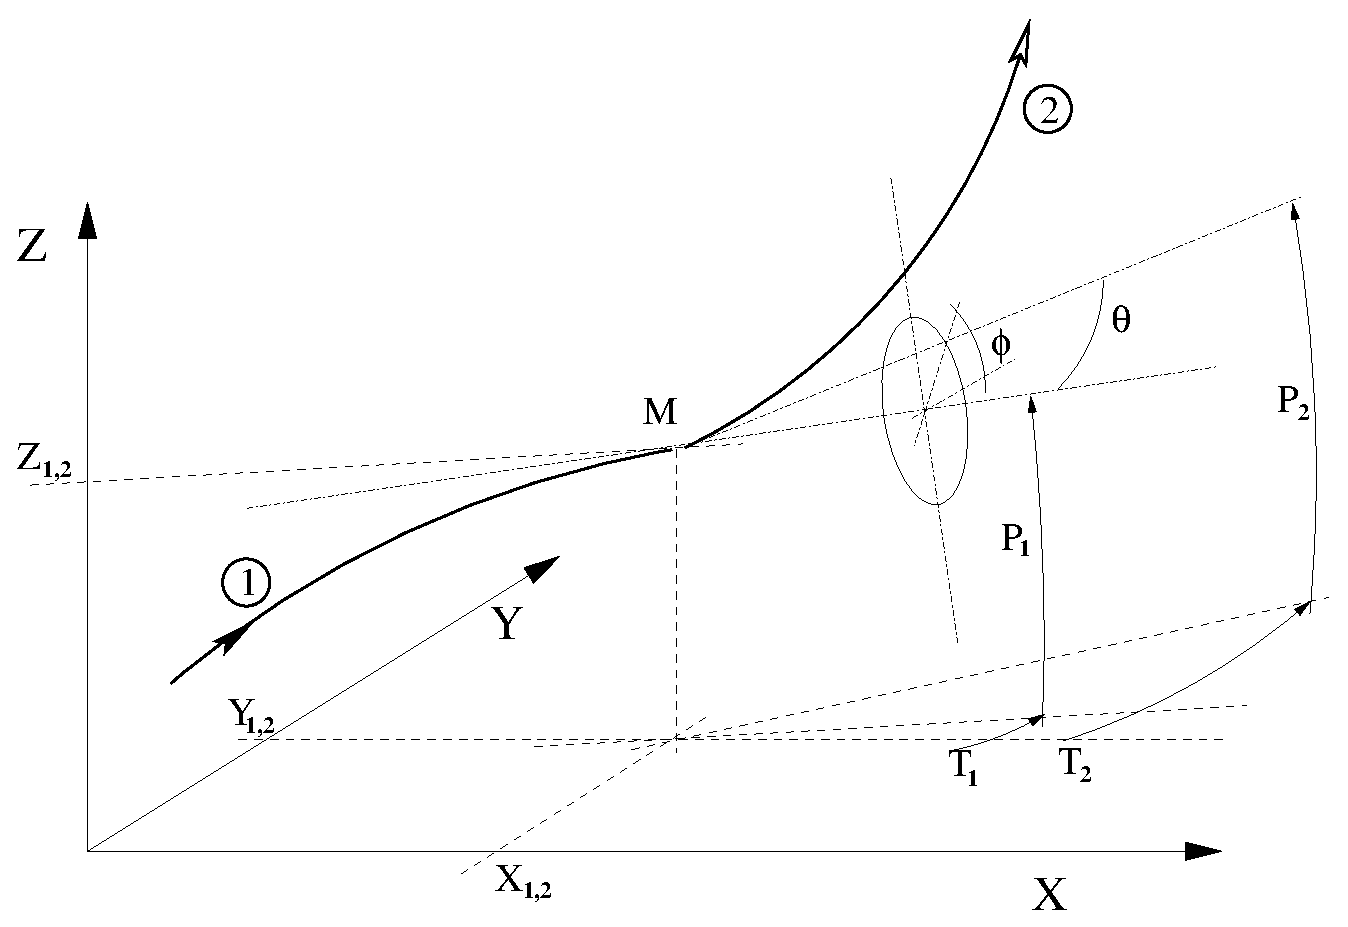
\includegraphics[height=12cm]{Fig6.eps}}
\unnumberedcaption{Particle 1 decays into 2 and 3~; \zgou\  then calculates 
trajectory of 2, while 3 is discarded. $\theta$ and $\phi$ are the scattering 
angles of particle 2 relative to the direction of the incoming 
particle 1. They transform to $ T_2 $ and $ P_2 $ in  Zgoubi  frame.}
\end{figure}
\vfill
 
\newpage

\begin{tabbing}
\mestab
~ ~ $ \omega^+$, $\theta$,     $R_1$, $U_1$, $U_2$, $R_2 $     \quad \=
 �$ B=\mathcal{F}B_0 \left(1+N \left(\frac{R-RM }{ RM} \right)      
                +B \left(\frac{R-RM}{ RM} \right)^2+G \left(\frac{R-RM }{ RM}
                \right) \right) $, more    \quad \= 2*cm, 2*deg, cm ~ \quad \= \kill
%%%%%%%%
\textbf{MCOBJET}         \label{MCOBJET-B} \index{MCOBJET|textbf}
   \> \textbf{\MCOBJETTitl}\index{Monte Carlo}
   \index{negative charge}\index{negative momentum} \> \> \\
 \\
 \\
 \textsl{BORO}\index{BORO@{\BORO}|textbf}      \>Reference rigidity \> kG.cm \>E\\
 \\
 \KOBJ      \>Type of support of the random distribution \>1-3 \>I \\
 \>\KOBJ = 1 :  window \> \> \\
 \>\KOBJ =  2 :  grid \>\>\\
 \>\KOBJ =  3 :  phase-space ellipses \>\>\\
  \\
 \IMAX\      \>Number of particles to be generated  \>$\leq \imax$ \>   \\
 \\
$KY$, $KT$, $KZ$, $KP$, \> Type of 
probability density \> 6*(1-3) \> 6*I\\
$KX$, $KD$~\footnotemark[1] \> \> \>\\
 \\
$ Y_0$, $T_0$, $Z_0$, $P_0$,  \>Mean value of coordinates  ($D_0=B\rho /\text{\BORO}$)  
         \>m, rad, m,\> 6*E\\
 $X_0$, $D_0 $       \> \>rad, m, no dim. \> \\
 \\
\textbf{If KOBJ = 1} \> \textbf{In a window} \> \> \\
\\
$\delta Y$, $\delta T$, $\delta Z$, $\delta P$, 
		\>Distribution widths, depending on $KY$, $KT$ 
		etc.~\footnotemark[1]
          \> m, rad, m, \>6*E\\
$\delta X$, $\delta D$  \>  \>rad, m, no dim. \> \\
 \\
$N_{\delta Y}$, $N_{\delta T}$, $N_{\delta Z}$, $N_{\delta P}$, 
	\> Sorting cut-offs (used only for Gaussian density) 
	\> units of $\sigma_Y$, $\sigma_T$, \> 6*E \\
$N_{\delta X}$, $N_{\delta D}$  \> \>  etc. \>\\
\\
$ N_0$, $C_0$, $C_1$, $C_2$, $C_3 $ \>Parameters involved in calculation of P(D)\>no 
dim. \>5*E \\
 \\
 $IR1$, $IR2$, $IR3$    \>Random sequence seeds \>3*$\simeq 10^6 $  \>3*I \\ 
\\
\textbf{If KOBJ = 2 } \>\textbf{On a grid}  \> \> \\  
 \\
 $IY$, $IT$, $IZ$, $IP$,     \>Number of bars of the grid \> \> 6*I \\
$IX$, $ID$ \> \> \> \\
 \\
$ PY$, $PT$, $PZ$, $PP$,    \>Distances between bars     \> m, rad, m \> 6*E\\
 $PX$, $PD$\>                           \> rad, m,  no dim.  \> \\
 \\
$ \delta Y$, $\delta T$, $\delta Z$, $\delta P$,    
		\>Width of the bars ($\pm$) if uniform, \> \ibidem  \>  6*E\\
$\delta X$,	$\delta D $ \>Sigma value if Gaussian distribution\>\>\\
 \\
$N_{\delta Y}$, $N_{\delta T}$, $N_{\delta Z}$, $N_{\delta P}$, 
	\> Sorting cut-offs (used only for Gaussian density) 
	\> units of $\sigma_Y$, $\sigma_T$,etc. \> 6*E \\
$N_{\delta X}$, $N_{\delta D}$  \> \> \>\\
 \\
$ N_0$, $C_0$, $C_1$, $C_2$, $C_3 $    \>Parameters involved in calculation of $ P(D) $ \>no
dim.   \>5*E\\
 \\
$ IR1$, $IR2$, $IR3$       \>Random sequence seeds \> 3*$\simeq 10^6 $ 
\>3*I\\ 
\end{tabbing}


\footnotetext[1]{~ Let $x= Y, T, Z, P \text{ or } X$. $KY$, $KT$, $KZ$, 
$KP$ and $KX$ can take the values
\begin{itemize}
\item[1 :] uniform, $p(x)=1/2\delta x$ if $-\delta x \leq x \leq \delta x$
\item[2 :] Gaussian, $p(x) = \exp (-x^2/ 2\delta x^2)/ \delta x \sqrt{2\pi}$
\item[3 :] parabolic, $p(x) =3(1-x^2 / \delta x^2)/ 4 \delta x$ if  
			$-\delta x \leq x \leq \delta x$
\end{itemize}			

 $KD$ can take the values
\begin{itemize}
\item[1 :] uniform, $p(D)=1/2\delta \! D$ if $-\delta \! D \leq x \leq \delta  \! D$
\item[2 :] exponential, $p(D) = \text{No }\exp (C_0 + C_1 l + C_2 l^2 + C_3 l^3)$
			if $-\delta D \leq x \leq \delta D$ 
\item[3 :] kinematic, $D= \delta D \ast T$
\end{itemize}}



\newpage
\begin{tabbing}
 \mestab
~ ~ $ \omega^+$, $\theta$,     $R_1$, $U_1$, $U_2$, $R_2 $     \quad \=
 �$ B=\mathcal{F}B_0 \left(1+N \left(\frac{R-RM }{ RM} \right)      
                +B \left(\frac{R-RM}{ RM} \right)^2+G \left(\frac{R-RM }{ RM}
                \right) \right) $, more    \quad \= 2*cm, 2*deg, cm ~ ~ \quad \= \kill
%%%%%%%%
\textbf{If KOBJ = 3} \label{pageMCOBJ3} \>\textbf{On a phase-space ellipse~\footnotemark[1]} \> \> \\
 \\
$ \alpha_ Y$, $\beta_ Y$, $\varepsilon_Y/\pi$, $N_{\sigma_{\epsilon_Y}} $   
		\>Ellipse parameters and    \>no dim., m/rad, \>4*E [,E] \\ 
{[}, $N'_{\sigma_{\epsilon_Y}}$ if $N_{\sigma_{\epsilon_Y}} < 0$]~\footnotemark[2]
		 \>emittance, Y-T phase-space~; cut-off \> m, units of  $\sigma(\varepsilon_Y)$\> \\
\\
$ \alpha_ Z$, $\beta_ Z$, $\varepsilon_ Z/\pi $, $ N_{\sigma_{\epsilon_Z}} $    
	\>Ellipse parameters and       \>no dim., m/rad, \>4*E [,E]  \\ 
{[}, $N'_{\sigma_{\epsilon_Z}}$ if $N_{\sigma_{\epsilon_Z}} < 0$]~\footnotemark[2]
		 \>emittance, Z-P phase-space~; cut-off    \>m, units of  $\sigma(\varepsilon_Z)$\> \\
 \\
$ \alpha_ X$, $\beta_ X$, $\varepsilon_ X/\pi $, $ N_{\sigma_{\epsilon_X}} $    
	\>Ellipse parameters and       \> no dim., m/rad, \>4*E [,E] \\ 
{[}, $N'_{\sigma_{\epsilon_X}}$ if $N_{\sigma_{\epsilon_X}} < 0$]~\footnotemark[2]
		 \>emittance, X-D phase-space~; cut-off  \>m, units of $\sigma(\varepsilon_X)$  \\ 
 \\
 $IR1$, $IR2$, $IR3$       \>Random sequence seeds    \>3*$\simeq 10^6 $\>3*I\\ 
\end{tabbing}

\footnotetext[1]{~ Similar possibilities, non-random, are offered with \textsl{OBJET}, KOBJ=8 
(p.~\pageref{pageOBJ8})} 
\footnotetext[2]{~ \begin{minipage}[t]{16cm}
Works with Gaussian density type only : sorting is within the ellipse frontier
$( \dfrac{1+\sigma^2_Y}{\beta^2_Y} Y^2 + 2 \alpha_Y YT + \beta_Y T^2 = \dfrac{\varepsilon_Y}{\pi})$
if $N_{\sigma_{\epsilon_Y}} > 0$, or,  if $N_{\sigma_{\epsilon_Y}} < 0$ sorting is within the annular region 
$ [\, |N_{\sigma_{\epsilon_Y}}|, N'_{\sigma_{\epsilon_Y}}\,]$ of that ellipse. 
\end{minipage}}

\newpage
\vfill
%%%%%%%%%%%%%%figure %%%%%%%%%%%%%
 \begin{figure}[H]
  % \vspace*{19 truecm}
\centerline{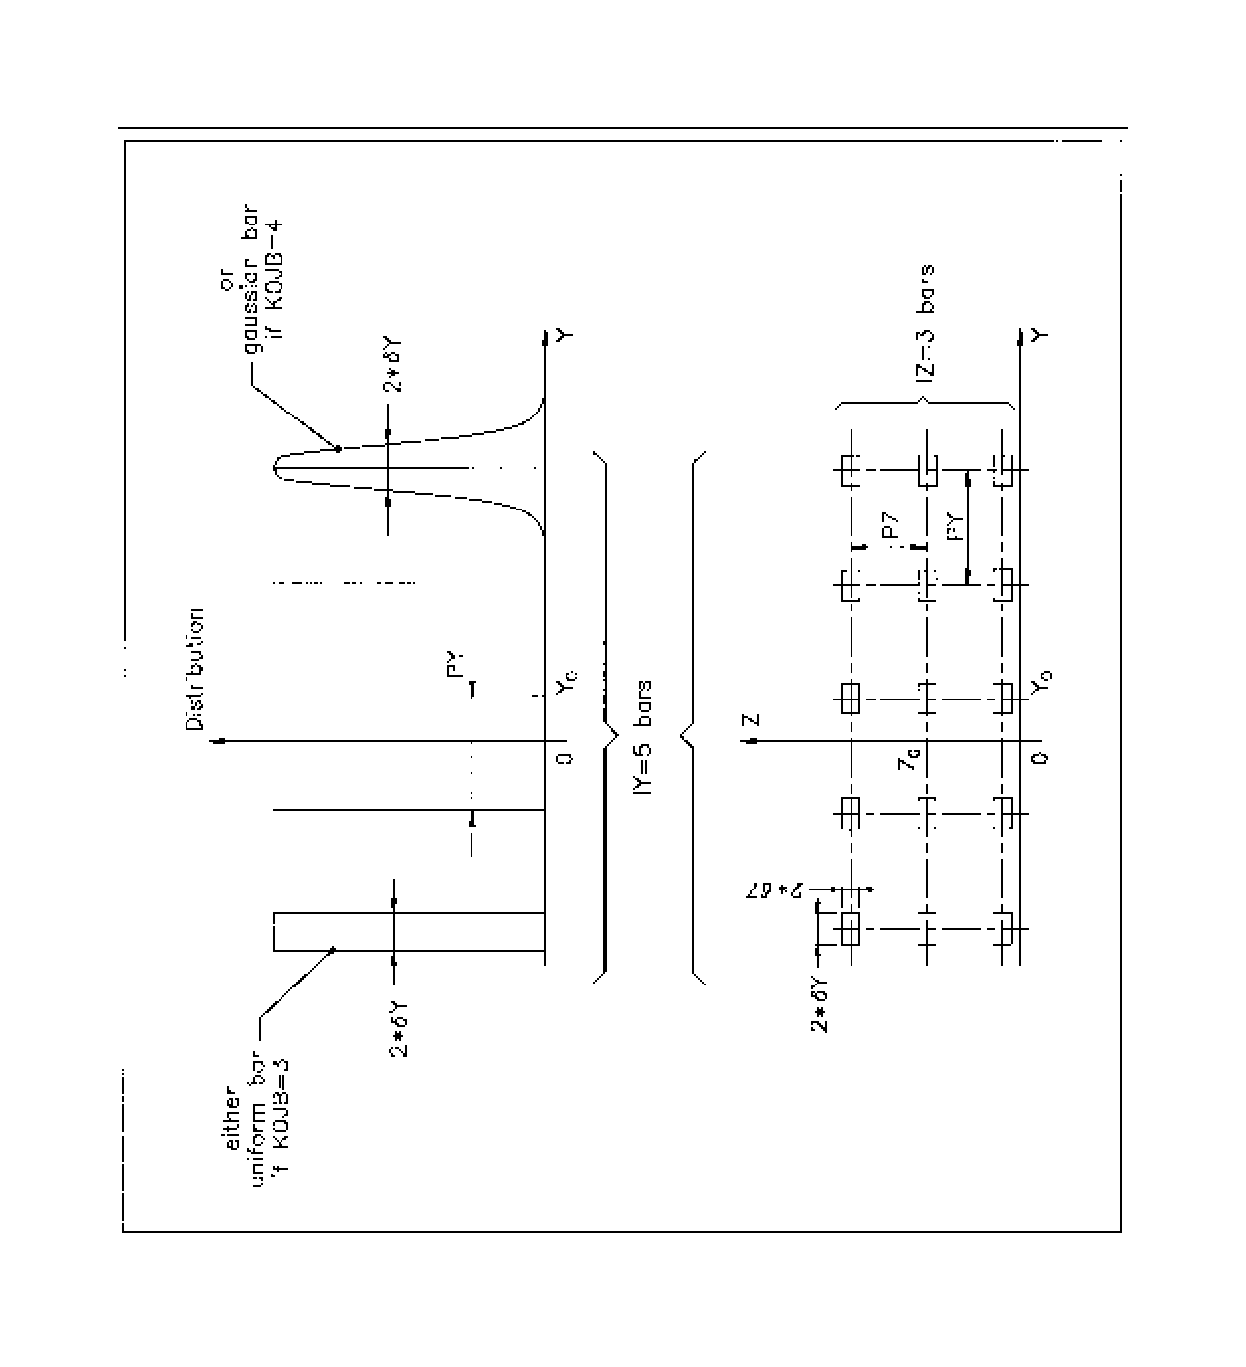
\includegraphics[height=15cm,angle=-90]{Fig5.ps}}
\unnumberedcaption{A scheme of  input parameters to \textsl{MCOBJET} when \KOBJ = 2. \\
   Top~: Possible  distributions  of the $ Y $ coordinate\\ 
Bottom~: A 2-D grid in ($ Y, Z $) space.
}
 \end{figure}
\vfill   

\newpage


\begin{tabbing}
 \mestab
 \textbf{MULTIPOL}        \label{MULTIPOL-B} \index{MULTIPOL|textbf}
           \> \textbf{Magnetic Multipole}  \> \> \\
 \\
 \\
 $\IL$   \>$\IL=1,2[\times 10^n],~7$ : print coordinates, fields, etc., along trajectories \>0-2$[\times 10^n]$, 7 \>I\\
        \> in zgoubi.res ($1$),  zgoubi.plt ($2$),  zgoubi.impdev.out ($7$).       \>                   \> \\
% $\IL$   \>$\IL=1,2[\times 10^n]$ : print field and coordinates along trajectories \>0-2$[\times 10^n]$ \>I\\
 \\
 $\XL$, $R_0$, $B1$, $B2$, ..., $B{10}$,  \>Length of element~; radius at pole tip~;
\>2*cm,10*kG \>12*E\\     
 \>field at pole tip for dipole, quadrupole, \>\>\\
 \>..., dodecapole components \>\>\\
 \\
 \>\textbf{Entrance face} \>\>\\
$ X_E$, $\lambda_E$, $E_2$, ..., $E_{10} $ \>Integration zone~; fringe field extent : 
\>2*cm,9*no dim.\> 11*E\\
 \>dipole fringe field extent = $ \lambda_ E $~; \>\>\\
 \>quadrupole fringe field extent = $ \lambda_ E\ast E_2 $~;\>\>\\
 \>...\>\>\\
 \>20-pole fringe field extent = $ \lambda_ E\ast E_{10} $ \>\>\\
 \>(sharp edge if field extent is zero) \>\>\\
 \\
 \textsl{NCE}, $ C_0-C_5 $            \>same as \textsl{QUADRUPO} 
 					\>0-6, 6*no dim. \>I, 6*E\\
 \\
 \>\textbf{Exit face} \>\>\\
$ X_S$, $\lambda_S$, $S_2$, ..., $S_{10} $ \>Integration zone~; as for entrance
         \>2*cm, 9*no dim. \> 11*E\\
 \\
 \textsl{NCS}, $ C_0-C_5 $           \> \> 0-6, 6*no dim. \>I, 6*E \\
 \\
$ R1$, $R2$, $R3$, ..., $R{10}$   \>Skew angles of field components \>10*rad \>10*E \\
\\
 \textsl{XPAS}                 \>Integration step    \>cm \>E \\
 \\
 \textsl{KPOS}, \textsl{XCE},   \textsl{YCE, ALE}     \>\textsl{KPOS}=1 : element aligned, 2 : misaligned~; shifts, tilt. 
           \>1-3,  2*cm, rad \>I, 3*E \\
\> \textsl{KPOS} = 3 : effective only if $B1 \not = 0$ :  \> \> \\ 
\> entrance and exit frames are shifted by \textsl{YCE} \> \> \\ 
\> and tilted \wrt\ the magnet by an angle  of          \> \> \\ 
\> $\bullet$ either ALE if ALE$\not =$0 \> \> \\ 
\> $\bullet$ or $2\, \textrm{Arcsin}( B1 \, \XL\, /\, 2 BORO)$ if ALE=0 \> \> \\ 

\end{tabbing}

\newpage

\begin{tabbing}
 \mestabOBJ
\textbf{OBJET}         \label{OBJET-B} \index{OBJET|textbf} \index{negative charge}\index{negative momentum}
          \>\textbf{Generation of an object} \> \> \\
 \\
 \\
 \BORO\index{BORO@{\BORO}|textbf}           \>Reference rigidity      \>kG.cm  \>E \\
 \\
 \textsl{KOBJ[.K2]}           \>Option index [.More options]            \>1-6    \>I \\
 \\
\textbf{If KOBJ = 1[.1]}      \> [Non-] Symmetric object \> \> \\
\\
 \textsl{IY, IT, IZ, IP, IS, ID}  
 \>Ray-Tracing assumes mid-plane symmetry. Generated points~:   \> {\footnotesize IY*IT*IZ*IP*IS*ID $\leq \imax$ } \> 6*1  \\
 \>$\YR\pm  IY\ast \dY$, $\TR\pm  IT\ast \dT$, $\ZR\pm  IZ\ast \dZ$, $\PR\pm  IP\ast \dP$ \> \> \\ 
		\> [$\ZR+  IZ\ast \dZ$, $\PR+\ IP\ast dP$ if KOBJ = 1.1], $\SR\pm  IS\ast \dS$    \> \>\\
 \>and $\DR \pm  ID\ast dD$ coordinates ($IY \leq 20$,...,$ID \leq 20$)   \> \>\\
 \\
 \textsl{dY, dT, dZ, dP, dS, dD}
       \>Sampling size in $Y$, $T$, $Z$, $P$, $S$ and in relative momentum   \>2(cm,mrad),  cm, no dim.  \> 6*E \\
 \>($\dD =  \delta B \rho /\text{\BORO}$)           \> \>  \\
 \\
\YR, \TR, \ZR, \PR, \SR, \DR    \>Reference trajectory ($\DR=B\rho/\text{\BORO}$)    \>2(cm,mrad),  cm, no dim.   \>  6*E \\
 \\
\textbf{If KOBJ = 2[.1]}      \>All the initial coordinates must be entered explicitly\>\>\\
\\
 \IMAX, \textsl{IDMAX}     \>total number of particles~; number of distinct momenta  
            \>\IMAX\ $\leq \imax$ \>2*I\\
 \>(if \textsl{IDMAX} $> 1$, group particles of same momentum)    \>\>\\
 \\
\textbf{For I = 1, IMAX}  \>Repeat \IMAX\ times the following line  \> \>\\
\\
 \textsl{Y, T, Z, P, S, D, LET} 
           \>Coordinates and tagging  of the \IMAX\ particles~; 
                                                         \>2(cm,mrad), cm, no dim.,   \>6*E, A1\\
            \> \textsl{If KOBJ = 2.1} input units are different~:  \>2(m,rad), m, no dim.,   \>\\
 \\
 \IEX($I=1$, \IMAX)  \>\IMAX\ times 1 or -9. If $\IEX(I)=1$ trajectory $I$ is   \>1 or -9  \>\IMAX\*I\\
                     \>   ray-traced, it is not if $\IEX(I)=-9$.   \> \> \\
 \\
\textbf{If KOBJ=3[.N, N=0 - 3]}      \>Reads coordinates from a storage file \> \> \\
                     \> N=0 (default) : [b\_]zgoubi.fai style data file FORMAT  \> \> \\
                     \> N=1 : read FORMAT is \texttt{\small``READ(NL,*) Y,T,Z,P,S,DP''}   \> \> \\
                     \> N=2 : read FORMAT is \texttt{\small``READ(NL,*) X,Y,Z,PX,PY,PZ''}   \> \> \\
                     \> N=3 : read FORMAT is \texttt{\small``READ(NL,*) DP,Y,T,Z,P,S,TIME,MASS,CHARGE''}   \> \> \\
 \\
 \textsl{IT1, IT2, ITStep}     \> Read particles numbered IT1 to IT2, step ITStep
              \> $\geq 1$, $\geq IT1$, $\geq 1$ \>3*I\\
 \>(For more than \imax\ particles stored in \textsl{FNAME}, \>\>\\
 \>use `\textsl{REBELOTE}')\index{REBELOTE} \>\>\\
 \\
 \textsl{IP1, IP2, IPStep}     \> Read particles that belong in pass numbered 
              \> $\geq 1$, $\geq IP1$, $\geq 1$ \>3*I\\
                               \> IP1 to IP2, step IPStep  \\
  \\
\textsl{YF, TF, ZF, PF,}    \> Scaling factor. TAG-ing letter : no effect if \textsl{TAG}='*',    \> 7*no.dim, char.\>  7*E, A1 \\
 \textsl{SF, DF, TF, TAG}  \> otherwise only particles with TAG$\equiv$LET are retained. \>     \>\\
  \\
\textsl{YR, TR, ZR, PR,}   \>Reference. Given the previous line of data,     \>2(cm, mrad), \>  7*E \\
\textsl{SR, DR, TR}       \> all coordinate C (=Y, T...) is transformed to C*CF+CR \> cm, no dim.,$\mu$s     \>\\
\\
 \textsl{InitC}     \> 0~: set new $\vec R_0 = \vec R_0$ as~read, new $\vec R = \vec R$ as~read~;      \> 0-1 \> I  \\
              \> 1 : set new $\vec R_0 = \vec R$ as~read, new $\vec R = \vec R$ as~read~; \\
              \> 2 : save $\vec R$ as~read in new $\vec R_0$, set new $\vec R = \vec R_0$ as~read. \\
 \\
 \textsl{FNAME}        \>File name (\emph{e.g.},  [b\_]zgoubi.fai\index{zgoubi.fai})  \> \>A80 \\
                       \> (N in KOBJ=3.N determines storage FORMAT)
\end{tabbing}

\newpage


\begin{tabbing}
 \mestabOBJ
%\textbf{If KOBJ = 4}      \> \textbf{Non symmetric object} \> \> \\
%\\
% $IY$, $IT$, $IZ$, $IP$,    \>Total number of points in $\pm Y$, $\pm T$, $+Z$, $+P$,
%               \> IY*IT*IZ*IP \> 6*I\\
%$IX$, $ID$\> $\pm X$ and $\pm D$ coordinates ($IY \leq 20$,...,$ID \leq 20$)   \>*IX*ID $\leq \imax$ \> \\
% \\
% $PY$, $PT$, $PZ$, $PP$,    \>Step sizes in $Y$, $T$, $Z$, $P$ $X$ and $D$.
%         \>2(cm,mrad), \>6 *E\\
% $PX$, $PD$\>                                    \>cm, no dim. \> \\
% \\
%$YR,TR,ZR,PR,$              \>Reference   \>2(cm,mrad), \>  6*E \\
%$XR,DR$              \> ($DR=B\rho/\text{\BORO}$) \>  cm, no dim.     \>\\
% \\

\textbf{If KOBJ = 5[.N, $N \geq 1$]} \>\textbf{Generation of 11 particles, or 11*N if $N\ge 2$}    (for use with \textsl{MATRIX}\index{MATRIX}, $IORD=1$)  \>\>\\
 \\
 \textsl{dY, dT, dZ, dP, dS, dD}  \>Sampling size in $Y$, $T$, $Z$, $P$, $S$ (unused) and $D$
                                              \>2(cm,mrad), cm, no dim. \> 6*E\\
 \\
 \textsl{YR, TR, ZR, PR, SR, DR} \> 
                        Reference trajectory   ($\DR= B \rho /\text{\BORO}$~; \SR\ is not sused)      \> 2(cm,mrad),  cm, no dim. \>  6*E  \\
 \\
\textsl{If KOBJ = 5.1}      \> additional data line :  \>\>\\
 $\alpha_Y, \beta_Y$, $\alpha_Z, \beta_Z$, $\alpha_S, \beta_S$,  \> Initial beam ellipse parameters~\footnotemark[1]  
         \> 2(no dim.,m),  ?, ?, \>  6*E, \\
 $D_Y, D_Y'$, $D_Z, D_Z'$  \>       \> 2(m,rad)\>  4*E \\
 \\
\textsl{If KOBJ = 5.N ($2\! \leq N \! \leq 99$)}
      \> i = 1 to N-1 additional data lines :  \>\>\\
 \textsl{YR, TR, ZR, PR, SR, DR}  \> 
                        Reference trajectory \# i  ($\DR= B \rho /\text{\BORO}$~; \SR\ is not sused)      \> 2(cm,mrad), cm, no dim.  \>  6*E  \\
 \\
\textbf{If KOBJ = 6}      \>\textbf{Generation of 61 particles}  (for use with \textsl{MATRIX}\index{MATRIX}, $IORD=2$)  \> \> \\
 \\
 \dY, \dT, \dZ, \dP, \dS, \dD \>Sampling size in $Y$, $T$, $Z$, $P$, $S$ (unused) and $D$
     \>2(cm,mrad),  cm, no dim.  \>6*E \\
 \\
 \textsl{YR, TR, ZR, PR, SR, DR} \> Reference trajectory~; $\DR= B \rho /\text{\BORO}$  \> 2(cm,mrad),  cm, no dim. \>   6*E\\
 \\
\textbf{If KOBJ = 7}      \>\textbf{Object with kinematics} \>\>\\
\\
  \textsl{IY, IT, IZ, IP, IS, ID}
       \>Number of points in $\pm Y$, $\pm T$,$\pm Z$, $\pm P$, $\pm S$~; $ID$ is not used  \> \textsl{IY*IT*IZ*IP*IS}$\leq\imax$ \> 6*I \\
 \\
 \dY, \dT, \dZ, \dP, \dS, \dD   \>Sampling size in $Y$, $T$, $Z$, $P$ and $S$~; $\dD$ = kinematic 
                                                                  \>2(cm,mrad),  cm, mrad$^{-1}$ \> 6*E\\
             \>coefficient, such that $ D(T)=DR+\dD \ast  T $ \>\>\\
 \\
 \textsl{YR, TR, ZR, PR, SR, DR}              \>Reference  ($DR=B\rho/\text{\BORO}$)  \>2(cm,mrad), cm, no dim. \>  6*E \\
 \\
\textbf{If KOBJ = 8} \label{pageOBJ8}     \>\textbf{Generation of phase-space coordinates on ellipses~\footnotemark[2]} \>\>\\
\\
 $IY$,  $IZ$, $IS$  
       \>Number of samples in each 2-D phase-space~;  \>  {\footnotesize $0\le IY,IZ,IS \le IMAX$}, \> 3*I\\
       \> if zero the central value (below) is assigned \>  {\footnotesize $1\le IY*IZ*IS \le IMAX$}\> \\
  \\
$Y_0$, $T_0$, $Z_0$, $P_0$, $S_0$, $D_0$\> Central values ($D_0 = B \rho /\text{\BORO}$)
	\> 2(m, rad), m, no dim. \> 6*E\\
\\
$\alpha_Y$, $\beta_Y$, $\varepsilon_Y/\pi$       
		\> ellipse parameters and emittances \> no dim., m, m  \> 3*E \\
$\alpha_Z$, $\beta_Z$, $\varepsilon_Z/\pi$ \>          \> no dim., m, m \> 3*E \\
$\alpha_S$, $\beta_S$, $\varepsilon_S/\pi$\>       \> no dim., m, m  \> 3*E \\


$\delta Y$, $\delta T$, $\delta Z$, $\delta P$, $\delta D$\quad \=
      Body to be tracked : $M3$(\textsl{IBODY} = 1), $M5$(\textsl{IBODY} = 2)\quad \=
            2(cm,mrad),  \quad \=  \kill

\end{tabbing}

\footnotetext[1]{~ They can be transported by using MATRIX}
\footnotetext[2]{~ Similar possibilities, random, are offered with \textsl{MCOBJET}, KOBJ=3 
(p.~\pageref{pageMCOBJ3})} 
%%%






\newpage


\noindent $\bullet$ \textbf{OBJET, \KOBJ=3} recovering from a crash~: An example  \label{ExaOBJ3Recovery}
\index{OBJET!- recovering from a crash}

\smallskip 

\noindent The job below, a 9 million turn tracking in RHIC, crashed at turn \# 2,217,299. 
It can be read from the storage file b\_zgoubi.fai (or infered as well from the \textsl{OBJET} 
and \textsl{CAVITE} data), that the reference (synchronous, theoretical) 
rigidity at the previously saved turn (turn\# 2,217,298, the closest integer multiple of 67) 
was  $B\rho_{\rm ref}=272.519214209$~T.m (magnet scaling coefficient under \textsl{SCALING}, right column below), 
which is $B\rho_{\rm ref} / \BORO = 3.111758007$ 
(as used in \textsl{SCALING}, \texttt{CAVITE} data, right column), with $\BORO=87.5772517$~T.m the initial rigidity (25.33~GeV), top of left column. 

\noindent The right column shows how these informations are transposed to the new tracking run based on 
\textsl{OBJET, \KOBJ=3}, which allows resuming tracking from that last saved turn \#2,217,298.  

~

\hspace{-7ex}
\begin{minipage}{0.499\linewidth}
\scriptsize
\begin{verbatim}
This 9,000,000-turn job crashed at turn number 2,217,299.
'OBJET'        
87.5772517e3                    
2              ! Declare 8 particles, all 
8 1            ! on a 21mu_m, norm. vertical invariant. 
0.     0.    2.58575455E-01  -1.73487148E-01  0. 1. 'o'   
0.     0.    1.82840458E-01   1.21643409E-01  0. 1. 'o'   
0.     0.    1.58331802E-17   3.45516907E-01  0. 1. 'o'   
0.     0.   -1.82840458E-01   3.66991287E-01  0. 1. 'o'   
0.     0.   -2.58575455E-01   1.73487148E-01  0. 1. 'o'   
0.     0.   -1.82840458E-01  -1.21643409E-01  0. 1. 'o'   
0.     0.   -4.74995405E-17  -3.45516907E-01  0. 1. 'o'   
0.     0.    1.82840458E-01  -3.66991287E-01  0. 1. 'o'   
1 -1 -1 -1 -1 -1 -1 -1  ! on/off switches. Particle 1 selected. 
'PARTICUL'        ! Particle data needed for spin tracking.
9.382720300E+02 1.602176487E-19 1.792847400  0. 0.  
'SPNTRK'     
3                 ! All initial spins vertical. 
'FAISCEAU'
'FAISTORE'        ! Storage location in sequence is at SNK1, 
b_zgoubi.fai SNK1 ! the first of the two helicoidal snakes. 
67                ! Storage (at pass 1 and) every 67 passes.
'SCALING'          
1  5              ! 5 families of magnets ramped. 
BEND              ! Magnet fields strictly follow cavity kick :
-1                ! (i) NT=-1 can be used, and (ii) CAVITE does 
87.5772517        ! not need be declared under SCALING.
1     
MULTIPOL HKIC VKIC              
-1    
0.                ! Zero field in HKIC and VKIC magnet families.
1     
MULTIPOL QUAD                   
-1    
87.5772517                      
1     
MULTIPOL SEXT                   
-1    
87.5772517                      
1     
MULTIPOL MULT                   
-1    
87.5772517                      
1
 'OPTIONS'
1 1   
WRITE OFF                       
'MARKER'   MARK      RHIC$START   
'MARKER'   MARK      CLOCK6down
------ RHIC ring, from CLOCK6 to CLOCK6 ------------
'MARKER'   MARK      CLOCK6up    
'MARKER'   MARK      RHIC$END   
'CAVITE'  accelerating cavity  
2     
3833.8456    120.00 circumf., H 
50e3    2.61799387799           
'REBELOTE'                     
8999999   0.4  99    ! Carry on tracking through optical 
                     ! sequence 8999999 times.
'END'
\end{verbatim}

\end{minipage} \hspace{4ex}
\begin{minipage}{0.47\linewidth}
This run recovers from the  crash, starting with particle, magnet and cavity  data as found at turn number 2,217,299. 
\scriptsize
\begin{verbatim}
 'OBJET'                        
87.5772517e3                    
3
1 8 1                    ! Will look for stored turn in 
2217290  2217299 1       ! range (2217298 is concerned). 
1. 1. 1. 1. 0. 1. 0. '*' ! Zero factor to 'S' for correct 
0. 0. 0. 0. 0. 0. 0.     ! path length/RF phase at CAVITE.
0
b_zgoubi.fai    ! The storage file is used to recover 
                ! particle coordinates at pass # 2217299.
'PARTICUL'                     
9.382720300E+02  1.602176487E-19  1.792847400E+00  0. 0.  
'SPNTRK'                       
3      
'FAISCEAU'                     

'FAISTORE'                     
b_zgoubi_rest.fai   SNK1   
67
'SCALING'               
1  6
BEND  
-1    
272.519214209                      
1     
MULTIPOL HKIC VKIC              
-1    
0.    
1     
MULTIPOL QUAD                   
-1    
272.519214209                      
1     
MULTIPOL SEXT                   
-1    
272.519214209                      
1     
MULTIPOL MULT                   
-1    
272.519214209                      
1     
CAVITE
2
1.            3.07555022085 
1             6782702

'OPTIONS'               
1 1   
WRITE OFF                        

'MARKER'  SNK1down  ! RHIC start changed to SNK1
------ RHIC ring, from snake 1 to snake 1 ------
'MARKER'   MULT      ERHLX                         
'MARKER'    SNK1up
'SPINR'    SNK1      OSNKE                        
1     
+45. 180.                ! snkAxis, spin angle 
'CAVITE'                 ! accelerating cavity                 
2     
3833.8456    120.00 
50e3    2.61799387799           
'REBELOTE'              
6782700   0.4  99                      
'END'                   
\end{verbatim}

\end{minipage}  




\newpage

\begin{tabbing}
 \mestabOBJ
\textbf{OBJETA}         \label{OBJETA-B} \index{OBJETA|textbf}
 \> \textbf{\OBJETATitl}\index{Monte Carlo} \> \>
\\
\\
 \> $M1+M2  \longrightarrow   M3+M4$ and $M4   \longrightarrow  M5+M6 $   \> \> \\
 \\
 \BORO\index{BORO@{\BORO}|textbf}            \>Reference rigidity                \>kG.cm \>E \\
 \>\>\>\\
 \textsl{IBODY, KOBJ}   \>Body to be tracked : $M3$ (\textsl{IBODY}=1), 
               $M5$ (\textsl{IBODY}=2) \>1-3,1-2 \>2*I\\
 \> $M6$ (\textsl{IBODY}=3)~; type of distribution for $ Y_0 $ and $ Z_0$ : \> \> \\
 \>uniform (\KOBJ = 1) or Gaussian (\KOBJ = 2) \> \> \\
 \\
 \IMAX\         \>Number of particles to be generated (use  \> $\leq \imax$ \>I \\
 \>`\textsl{REBELOTE}' for more) \>\>\\
 \\
$ M_1-M_6 $        \>Rest masses of the bodies           \> 6*GeV/c$ ^2 $\>6*E\\
 \\
$ T_1 $           \>Kinetic energy of incident body      \> GeV \> E \\
 \\
$ Y_0$, $T_0$, $Z_0$, $P_0$, $D_0 $ \>Only those particles in the range  \>2(cm,mrad),  
            \>5*E\\
 \>     $ Y_0-\delta Y\leq Y\leq Y_0+\delta Y $                 \> no dim. \> \\
 \>     \qquad\qquad   ........  \>\>\\
 \>     $ D_0-\delta D\leq D\leq D_0+\delta D $  \> \> \\
 \> will be retained \> \> \\
 \\
$\delta Y$, $\delta T$, $\delta Z$, $\delta P$, $\delta D$ \> \>2(cm,mrad),   \>5*E \\
 \> \> no dim.  \> \\
 \\
 $\XL$             \>Half length of object : $-\XL \leq X_0  \leq \XL$ \>cm \>E\\
 \> (uniform random distribution) \> \> \\
 \\
 $IR1$, $IR2$        \>Random sequence seeds  \> 2*$\simeq 0^6 $ \> 2*I   
\end{tabbing}

\newpage

\begin{tabbing}
\mestab
\textbf{OCTUPOLE}         \label{OCTUPOLE-B} \index{OCTUPOLE|textbf}
        \> \textbf{\OCTUPOLETitl}    \> \> \\
 \\
 $\IL$   \>$\IL=1,2[\times 10^n],~7$ : print coordinates, fields, etc., along trajectories \>0-2$[\times 10^n]$, 7 \>I\\
        \> in zgoubi.res ($1$),  zgoubi.plt ($2$),  zgoubi.impdev.out ($7$).       \>                   \> \\
% $\IL$  \>$\IL=1,2[\times 10^n]$ : print field and coordinates along trajectories. \>0-2$[\times 10^n]$\>I\\
 \\
 $\XL$, $R _0$, $B_0 $ \>Length~; radius and field at pole tip of the element \>2*cm, kG \>3*E\\
 \\
 \>\textbf{Entrance face : }\>\>\\
$ X_E$, $\lambda_E $    \>Integration zone~;   \> 2*cm  \>2*E \\
 \>Fringe field extent ($ \lambda_ E =0$ for sharp edge)\>\>\\
 \\
 \textsl{NCE}, $C_0-C_5 $ \>\textsl{NCE} = unused     \>any, 6*no dim. \>I, 6*E\\
 \>$C_0- C_5 $ = fringe field coefficients            \> \> \\
 \>such that : $ G(s)=G_0/(1+ \exp\ P(s))$,  with $ G_0=B_0/R^3_0 $ \>\>\\
 \>and $ P(s)= \sum^ 5_{i=0}C_i(s/\lambda )^i $  \>\>\\
 \\
 \> \textbf{Exit face :} \>\>\\
$ X_S$, $\lambda_ S $     \>Parameters for the exit fringe field~; see entrance \>2*cm \>2*E\\
 \\
 \textsl{NCS}, $C_0- C_5 $ \>  \> 0-6, 6*no dim. \>I, 6*E \\
 \\
 \textsl{XPAS}          \>Integration step  \>cm \>E \\
 \\
 \textsl{KPOS}, \textsl{XCE},    \textsl{YCE, ALE}     \>\textsl{KPOS}=1 : element aligned, 2 : misaligned~; shifts, tilt. 
           \>1-2, 2*cm, rad \>I, 3*E \\
\end{tabbing}

\vfill
%%%%%%%%%%%%%%figure%%%%%%%%%%%%%%
\begin{figure}[H]
%\vspace{12 truecm}
%%%Figure 24
\centerline{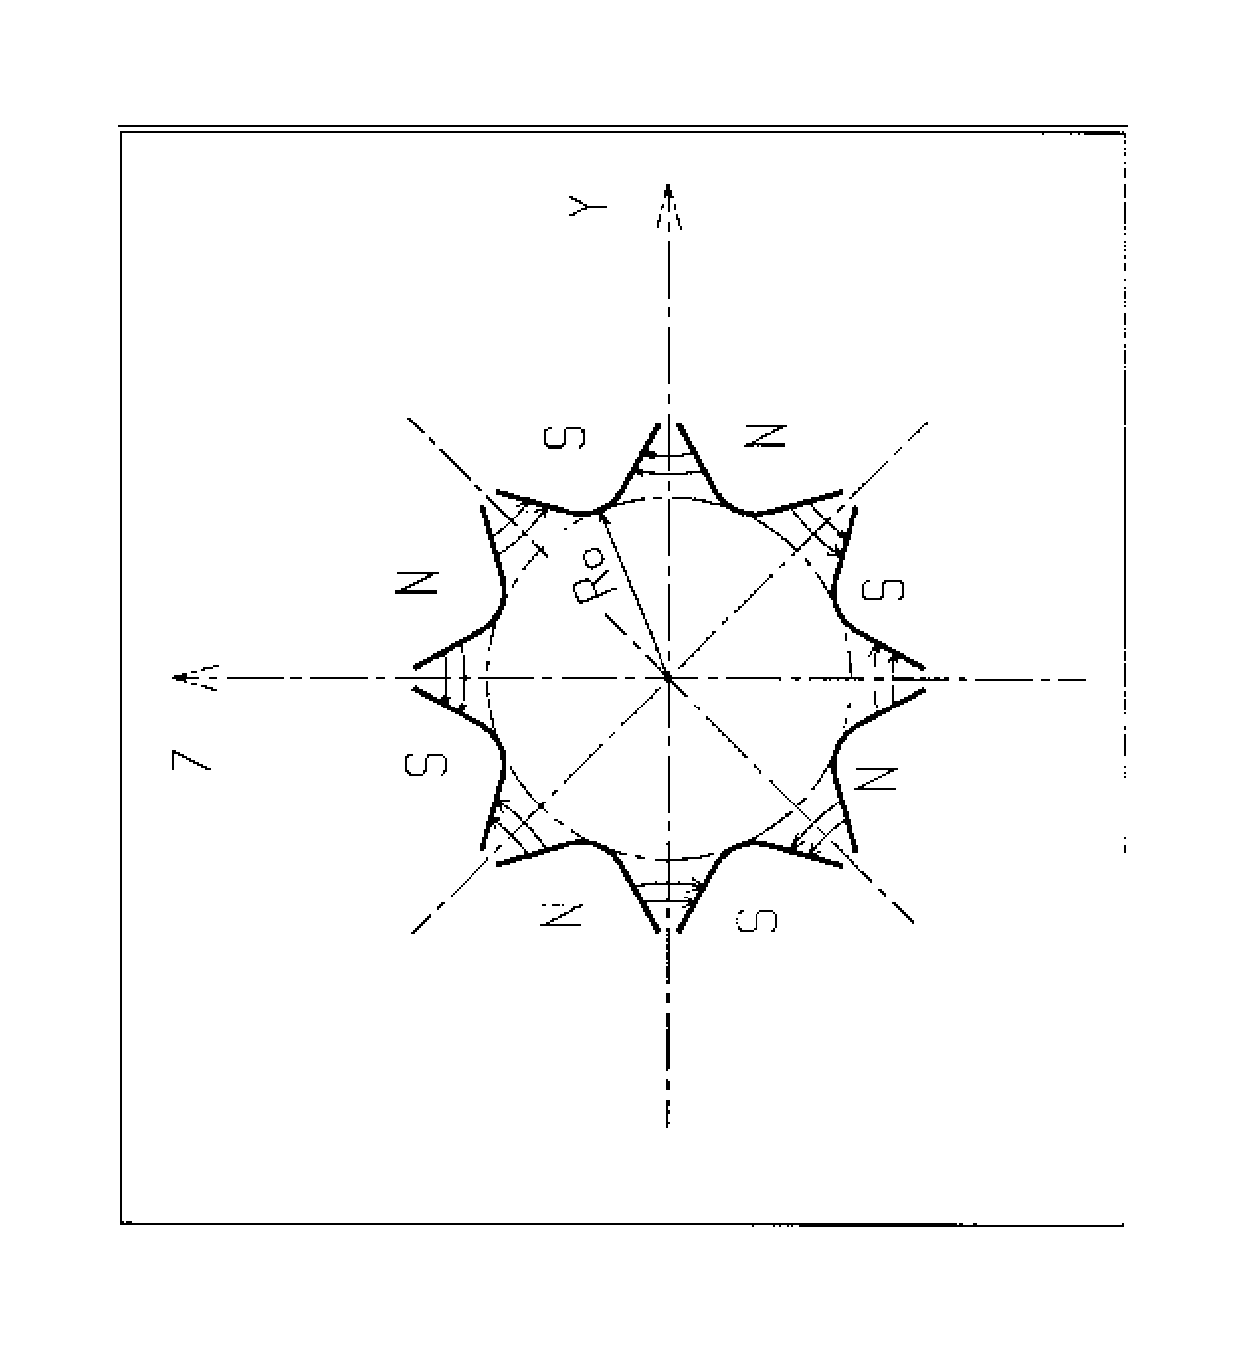
\includegraphics[height=10cm,angle=-90]{Fig24.ps}}
\unnumberedcaption{Octupole magnet}
\end{figure}
\vfill







\newpage


\begin{tabbing}
\mestab
\textbf{OPTICS}         \label{OPTICS-B} \index{OPTICS|textbf}
  \> \textbf{\OPTICSTitl }   \> \> \\
  \\
  \\
 \> \\[20pt]
%
%
 \textsl{IOPT[.NLBL]}, label(s) \> $IOPT=0/1$~: Off/On~; NLBL = number of labels (default is 1)~;  \> 0-1[.1-{\small NLBL}], - ,  \>I[.I],  \\
 \textsl{[, IMP or 'PRINT']} \> 'label'~:  can be  'all', 'ALL', or a list of \textsl{NLBL} first label(s) as   \> - , - \> 1-NLBL*A10, \\
\textsl{[, coupled]}        \> appearing at one or more elements in zgoubi.dat sequence~;  \>  \> I1 or A5, A7  \\
      \> wild card  accepted, in the form \textsl{'*myLabel'} or \textsl{'myLabel*'}.   \>  \> \\
      \> $IMP=1$, or presence of   'PRINT', will  cause storage of optical     \>  \> \\
      \>   functions  in zgoubi.OPTICS.out~; optical function computation is    \>  \> \\
      \>  in coupled hypothesis if specified, uncoupled otherwise.  \>  \> \\
\end{tabbing}


\vfill

{\noindent $\bullet$  {\bf \textsl{Example}} 
\\
\noindent The following will cause a print  of transported optical functions in zgoubi.res,  
at all optical elements of the zgoubi.dat sequence,  as well as their print out in zgoubi.OPTICS.out~: 
\begin{verbatim}
'OPTICS'
 1  all  PRINT
\end{verbatim}







\newpage


\begin{tabbing}
\mestab
$R_1$, $U_1$, $U_2$, $R_2 $     \quad \quad \=
 $ B=\mathcal{F}B_0 \left(1+N \left(\frac{R-RM }{ RM} \right)      
                +B \left(\frac{R-RM}{ RM} \right)^2+G \left(\frac{R-RM }{ RM}
                \right) \right) $    \quad \quad \quad \= 
        2*cm, 2*deg, cm ~ ~  \quad  \quad \quad \quad \quad \= \kill
%%%%
\textbf{OPTIONS}         \label{OPTIONS-B} \index{OPTIONS|textbf}
  \> \textbf{\OPTIONSTitl }   \> \> \\
  \\
  \\
 \> \\[20pt]
%
%
 \textsl{IOPT, NBOP}         \> $IOPT=0/1$~: Off/On~; 0 (off) will inhibit all \textsl{NBOP} subsequent  \>0-1, $\geq 0$ \>2*I \\
                             \>   requests. \textsl{NBOP}~: total number of options.   \>               \>    \\
      \>  \\
\sl  NBOP lines should follow. Possible choices :    \>  \\
\\
 \sl 'WRITE', OPT \> OPT = ON/OFF~: allows/inhibites (most) write statements to zgoubi.res  \> 'WRITE', 'ON' or 'OFF' \> 2*A \\
\\
\sl 'CONSTY', OPT \> OPT = ON~: forces constant $Y$ and $Z$ across optical elements  \> 'CONSTY', 'ON' or 'OFF' \> 2*A \\

\end{tabbing}




\newpage

\begin{tabbing}
$ \omega^+$, $\theta$, $R_1$, $U_1$, $U_2$, $R_2 $ \quad \=
$IO=4$ : (default option) expansions of $ \vec  R $ and $ \vec  u $ up to $ \vec u^{(4)} $ \qquad \= 2*cm, 2*deg, cm\quad  \= \kill
 %%%%
\textbf{ORDRE}         \label{ORDRE-B} \index{ORDRE|textbf} 
       \> \textbf{\ORDRETitl} \> \> \\
 \\
 \\
 $IO$        \>Taylor expansions of $ \vec  R $ and $ \vec  u $ up to $ \vec u^{(IO)} $  \> 2-5 \>I \\
      \> (default is  $IO=4$ )\>  \> \\

\end{tabbing}


\newpage

\begin{tabbing}
 $ \omega^+$, $\theta$,     $R_1$, $U_1$, $U_2$    \=
 �$ B=\mathcal{F}B_0 \left(1+N \left(\frac{R-RM }{ RM} \right)      
                +B \left(\frac{R-RM}{ RM} \right)^2+G \left(\frac{R-RM }{ RM}
                \right) \right) $  \quad \quad \quad \quad \= 
                   2*cm, 2*deg, cm ~ ~ \quad \quad \quad \quad \quad \= \kill
%%%%%%%%
\textbf{PARTICUL} \label{PARTICUL-B} \index{PARTICUL|textbf} 
\>\textbf{\PARTICULTitl } \> \> \\
  \\
  \\
\textbf{Either :} \\[1ex]
 $M$, $Q$, $G$, $\tau$, $X$  \>Mass~(or coded, see Note below)~; charge~; gyromagnetic factor~; 
              \>MeV/c$^2$, C, no dim., s, NA\>5*E\\
            \> COM life-time~; unused  \\
\\
\textbf{or :} \\[1ex]
Type      \> ELECTRON or MUON+, MUON-, PROTON \>  \> A
\end{tabbing}
\bigskip 
\bigskip 
\bigskip 

\noindent Note~: If $M$ is of the form \texttt{\{M1 M2\}}, then when masses are
assigned to particles from a previously defined object, the first half of
the particles are given the mass \texttt{M1}, and the second half are given
the mass \texttt{M2}.

\medskip
\noindent If $Q$ is zero, the reference charge is left unchanged.

\medskip
\noindent Only the parameters to be used need their value be specified (for 
instance $M$, $Q$ only when electric lenses are used,  $M$, $Q$, $G$ only when tracking spin)~; unused parameters
 can be set to zero. 






\newpage

\begin{tabbing}
\mestab
\textbf{PICKUPS}         \label{PICKUPS-B} \index{PICKUPS|textbf}         \> \textbf{\PICKUPSTitl}  \> \> \\
 \> \textbf{Summation of particles coordinates at pickups may be printed out in zgoubi.PICKUP.out.} \> \>  \\
 \> \textbf{Pickup contents are zeroed at start of each pass, in multi-turn mode.} \> \>  \\
 \\
 \\
 $N$       \> 0 : inactive \> \> \\
 \> $\geq 1$ : number of \textsl{LABELs} \index{LABEL@{\LABEL}}  at which beam centroid is computed \>  $\geq 0$ \>I \\
 \> 
 \\
  \\
\textbf{A list of N keywords' labels follows} \> \>\>\\
 \\
 \LABEL1 [,LABEL2, [...]]
          \> The N label(s) at which beam data are to be computed/recorded. \> N string(s) \> N*A10 \\
          \> If some ``\textsl{LABELi}'' in this list actually does not appear    \> \> \\
          \> in zgoubi.dat optical sequence, then it is peacefully ignored~; \>  \> \\
          \> wild card accepted, in the form \textsl{'*myLabel'} or \textsl{'myLabel*'}. \> \> \\
 \\
\end{tabbing}



\vfill

{\noindent $\bullet$  {\bf \textsl{Example}} 
\\
A trick~: 
{\small
\begin{verbatim}
'PICKUPS'  
1           
none labelA labelB ...
\end{verbatim}
}
\noindent This is a possible way to inhibit an earlier use of  \textsl{PICKUPS} with  ``labelA, labelB, ...'' 
keyword list. 
It is sufficient (and necessary) for that, that no keyword in zgoubi.dat data list have 
``none'' as its first \LABEL.  \index{LABEL}
}



\newpage


\begin{tabbing}
\mestab
\textbf{PLOTDATA}\label{PLOTDATA-B} \index{PLOTDATA|textbf} 
 \> \textbf{\PLOTDATATitl} \\
 \\
 \\
 \>  \textsl{To be documented.}
\end{tabbing}






\newpage

\begin{tabbing}
$ID$, $A$, $B$, $C$, ~�~�~ \qquad \quad  \= $ID=2$ : entrance ($A,B,C$) and exit ($A',B',C'$) integration
        \qquad \quad  \=  -1-2*no dim., cm \quad \quad \= \kill
%%%
\textbf{POISSON}         \label{POISSON-B} \index{POISSON|textbf}
      \>\textbf{\POISSONTitl} \>\>\\
 \\
 \\
 $\IC$, $\IL$      \>$\IC=1,2$ : print the field map \>0-2; 0-2$[\times 10^n]$, 7 \>2*I\\
  \>$\IL=1,2[\times 10^n],~7$ : print coordinates, fields, etc., along trajectories \> \>   \\
        \> in zgoubi.res ($1$),  zgoubi.plt ($2$),  zgoubi.impdev.out ($7$).       \>                   \> \\
% \>$\IL=1,2[\times 10^n]$ : print field and coordinates along trajectories. \> \> \\
 \\
 \textsl{BNORM, XN,YN}      \> Field and X-,Y-coordinate normalization  coeffs.   \> 3*no dim. \> 3*E \\
 \\
 \textsl{TITL}        \>Title. Start with ``FLIP'' to get field map X-flipped  \> \>A80 \\
 \\
 $IX$, $IY$       \>Number of longitudinal and transverse nodes\> $\leq 400$, $\leq 200$
         \>2*I\\
 \> of the uniform mesh \> \> \\
 \\
 \textsl{FNAME~\footnotemark[1]}    \>File name  \> \>A80 \\
 \\
 $ID$, $A$, $B$, $C$   \>Integration boundary. Ineffective when $ID=0$.      \>$\geq -1$, 2*no dim., \>I,3*E  \\
 {[}, $A'$, $B'$, $C'$,   \>$ID=$ -1, 1 or $\geq 2$ : as for  \textsl{CARTEMES} \> cm {[},2*no dim.,\>[,3*E,etc.]\\
 $B''$, etc., if $\left. ID\geq 2\right]$ \>                                  \> cm, etc.]       \> \\
 \\
 \textsl{IORDRE}     \> Degree of interpolation polynomial  \>2, 25 or 4 \>I\\
 \>as for \textsl{DIPOLE-M}\index{DIPOLE-M} \>\>\\
 \\
 \textsl{XPAS}          \>Integration step  \>cm \>E \\
 \\
 \textsl{KPOS}, \textsl{XCE},     \textsl{YCE, ALE}       \>\textsl{KPOS}=1 : element aligned, 2 : misaligned~; shifts, tilt. 
           \>1-2, 2*cm, rad \>I, 3*E \\
 \end{tabbing} 


\begin{alltt}
\footnotetext[1]{ \textrm{\textsl{FNAME} (\emph{e.g.}, ``outpoi.lis'')  contains the field map data. 
These must be formatted according to the following \textsl{FORTRAN} read sequence  - details 
and possible updates are to be found in the source  file \texttt{'fmapw.f'} :} 

       I = 0
   11  CONTINUE
       I = I+1
       READ(LUN,101,ERR=99,END=10) K, K, K, R, X(I), R, R, B(I) 
101	   FORMAT(I1, I3, I4, E15.6, 2F11.5, 2F12.3)
       GOTO II     
 10    CONTINUE
 
\textrm{where \(X(I)\) is the longitudinal coordinate, and \(B(I)\) is the \(Z\) component of the field at a node \((I)\) of the mesh. 
\(K\)'s and \(R\)'s are variables appearing in the \textsl{POISSON} output file outpoi.lis, not used here.} } 
\end{alltt}



\newpage

\begin{tabbing}  
\mestab
\textbf{POLARMES} \label{POLARMES-B} \index{POLARMES|textbf}
        \>\textbf{\POLARMESTitl }\> \> \\  
\>mid-plane symmetry is assumed \>\>\\
 \\
 \\
 $\IC$, $\IL$      \>$\IC=1,2$ : print  the map \>0-2; 0-2$[\times 10^n]$, 7 \>2*I\\
   \>$\IL=1,2[\times 10^n],~7$ : print coordinates, fields, etc., along trajectories \> \>   \\
        \> in zgoubi.res ($1$),  zgoubi.plt ($2$),  zgoubi.impdev.out ($7$).       \>                   \> \\
% \>$\IL=1,2[\times 10^n]$ : print field and coordinates along trajectories.  \> \> \\
 \\
  \textsl{BNORM, AN,RN}      \> Field and A-,R-coordinate normalization  coeffs.     \> 3*no dim. \> 3*E \\
 \\
 \textsl{TITL}        \>Title. Start with ``FLIP'' to get field map X-flipped  \> \>A80 \\
 \\
 $IA$, $JR$      \>Number of angular  and radial nodes of the mesh \>$\leq 400$, $\leq 200$ \>2*I \\
 \\
\textsl{FNAME}~\footnotemark[1] \> File name  \> \>A80 \\
 \\
 $ID$, $A$, $B$, $C$   \>Integration boundary. Ineffective when $ID=0$.      \>$\geq -1$, 2*no dim., \>I,3*E  \\
 {[}, $A'$, $B'$, $C'$,   \>$ID=$ -1, 1 or $\geq 2$ : as for  \textsl{CARTEMES} \> cm {[},2*no dim.,\>[,3*E,etc.]\\
 $B''$, etc., if $\left. ID\geq 2\right]$ \>                                  \> cm, etc.]       \> \\
 \\
 \textsl{IORDRE}     \> Degree of interpolation polynomial  \>2, 25 or 4 \>I\\
 \>(see \textsl{DIPOLE-M}) \>\>\\
 \\
 \textsl{XPAS}       \>Integration step    \> cm \>E \\
 \\
 \textsl{KPOS}    \>as for \textsl{DIPOLE-M}. Normally 2.    \>1-2  \>I \\
 \textbf{If KPOS = 2} \> \> \> \\
 $RE$, $TE$, $RS$, $TS$ \> \> cm, rad, cm, rad \> 4*E \\
 \textbf{If KPOS = 1} \> \> \> \\
 $DP$ \> \> no dim. \> E 
\end{tabbing}

 

\begin{alltt}
\footnotetext[1]{ \textrm{ \textsl{FNAME} (\emph{e.g.},  spes2.map) contains the field data. 
These must be formatted according to the following \textsl{FORTRAN} read sequence  - details 
and possible updates are to be found in the source  file \texttt{'fmapw.f'} :}

	      OPEN (UNIT = NL, FILE = FNAME, STATUS = `OLD' [,FORM='UNFORMATTED'])
	      IF (BINARY) THEN 
	        READ(NL) (Y(J), J=1, JY)
	      ELSE
                READ(NL,100) (Y(J), J=1, JY)
              ENDIF
     100      FORMAT(10 F8.2)	
              DO 1 I = 1,IX
	        IF (BINARY) THEN 
	          READ	(NL) X(I), (BMES(I,J), J=1, JY)
	        ELSE
	          READ(NL,101) X(I), (BMES(I,J), J=1, JY) 
     101	  FORMAT(10 F8.1)
                ENDIF
        1     CONTINUE

\textrm{where \(X(I)\) and \(Y(J)\) are the longitudinal and transverse coordinates and \textsl{BMES} is the \(Z\) field component  at a node \((I,J)\) 
of the mesh. For binary files, \textsl{FNAME} must begin with 'B\(\sb{_}\)' or 'b\(\sb{_}\)'. `Binary' will then automatically be set to `.TRUE.'}
}
\end{alltt}
\newpage

\begin{tabbing}
\mestab
 \textbf{PS170}        \label{PS170-B} \index{PS170|textbf}
          \>\textbf{\PSusoTitl} \>\>\\
 \\
 \\
 $\IL$   \>$\IL=1,2[\times 10^n],~7$ : print coordinates, fields, etc., along trajectories \>0-2$[\times 10^n]$, 7 \>I\\
        \> in zgoubi.res ($1$),  zgoubi.plt ($2$),  zgoubi.impdev.out ($7$).       \>                   \> \\
% $\IL$   \>$\IL=1,2[\times 10^n]$ : print field and coordinates along trajectories. \>0-2$[\times 10^n]$ \>I\\
 \\
 $\XL$, $R_0$, $B_0 $ \>Length of the element, radius of the circular \>2*cm, kG \>3*E\\
 \>dipole, field \>\>\\
 \\
 \textsl{XPAS}          \>Integration step  \>cm \>E \\
 \\
 \textsl{KPOS}, \textsl{XCE},   \textsl{YCE, ALE}     \>\textsl{KPOS}=1 : element aligned, 2 : misaligned~; shifts, tilt.
           \>1-2, 2*cm, rad \>I, 3*E \\
% \textsl{YCE, ALE}      \>shifts, tilt (unused if \textsl{KPOS}=1)  
\end{tabbing}

\vfill

%%%%%%%%%%%%%%figure%%%%%%%%%%%%%%
\begin{figure}[H]
%\vspace{17 truecm}
%%%Figure 25
\centerline{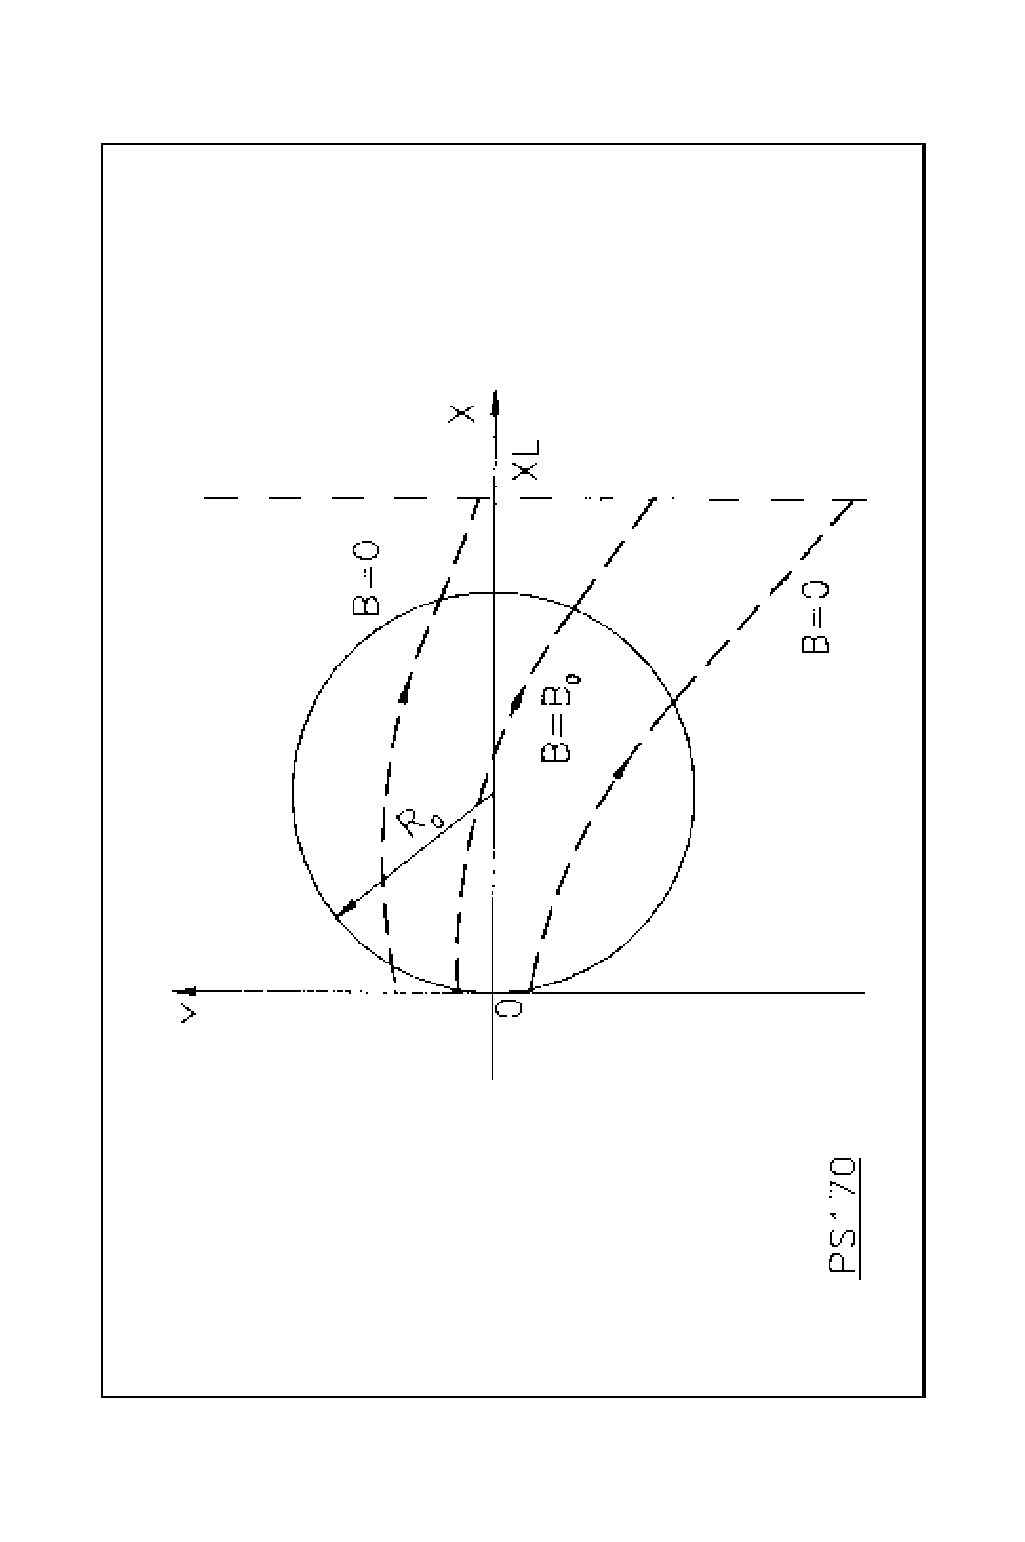
\includegraphics[height=15cm,angle=-90]{Fig25.ps}}
\unnumberedcaption{Scheme of the PS170 magnet simulation.}
\end{figure}

\vfill
\newpage

\begin{tabbing}
$ N$, $EB1$, $EB2$, $EG1$, $EG2$\quad \= 
    $\IL=1,2[\times 10^n]$, 7 : print field and coordinates along trajectories. ~ ~ ~ ~ \quad \=
        1-2, 2*cm, rad\quad \= \kill
%%%
\textbf{QUADISEX}         \label{QUADISEX-B} \index{QUADISEX|textbf}
      \>  \textbf{\QUADISEXTitl}  \> \> \\
 \>$ B_Z\mid_{ Z=0}=B_0 \left(1+\dfrac{N}{R_0} Y + \dfrac{B}{R^2_0} Y^2 + 
              \dfrac{G}{R^3_0} Y^3 \right) $  \> \> \\
 \\
 \\
 $\IL$   \>$\IL=1,2[\times 10^n],~7$ : print coordinates, fields, etc., along trajectories \>0-2$[\times 10^n]$, 7 \>I\\
        \> in zgoubi.res ($1$),  zgoubi.plt ($2$),  zgoubi.impdev.out ($7$).       \>                   \> \\
%$\IL$            \>$\IL=1,2[\times 10^n]$ : print field and coordinates along trajectories. \>0-2$[\times 10^n]$ \>I\\
 \\
 $\XL$, $R_0$, $B_0 $ \>Length of the element~; normalization distance~; field \>2*cm, kG \>3*E\\
 \\
$ N$, $EB1$, $EB2$, $EG1$, $EG2$ \>Coefficients for the calculation of B. \>5*no dim. \>5*E\\
 \>if $Y > 0$ : $B=EB1$ and $G=EG1$~; \>\>\\
 \>if $Y < 0$ : $B=EB2$ and $G=EG2$. \>\>\\
 \\
 \textsl{XPAS}          \>Integration step  \>cm \>E \\
 \\
 \textsl{KPOS}, \textsl{XCE},    \textsl{YCE, ALE}      \>\textsl{KPOS}=1 : element aligned, 2 : misaligned~; shifts, tilt. 
           \>1-2, 2*cm, rad \>I, 3*E \\
% \textsl{YCE, ALE}      \>shifts, tilt (unused if \textsl{KPOS}=1)  
\end{tabbing}
\newpage

\begin{tabbing}
\mestab
 \textbf{QUADRUPO}        \label{QUADRUPO-B} \index{QUADRUPO|textbf}
  \> \textbf{\QUADRUPOTitl }  \> \> \\
 \\
  \\
 $\IL$   \>$\IL=1,2[\times 10^n],~7$ : print coordinates, fields, etc., along trajectories \>0-2$[\times 10^n]$, 7 \>I\\
        \> in zgoubi.res ($1$),  zgoubi.plt ($2$),  zgoubi.impdev.out ($7$).       \>                   \> \\
% $\IL$        \>$\IL=1,2[\times 10^n]$ : print field and coordinates along trajectories. \>0-2$[\times 10^n]$ \>I \\
 \\
 $\XL$, $R_0$,$B_0 $ \>Length~; radius and field at pole tip \>2*cm, kG \>3*E \\
 \\
 \>\textbf{Entrance face :} \>\>\\
$ X_E$, $\lambda_ E $    \>Integration zone extent~; fringe field \>2*cm \>2*E \\
 \>extent ($\simeq 2 R_0$, $\lambda_ E=0 $ for sharp edge) \>\>\\
 \\
 \textsl{NCE}, $ C_0-C_5 $ \>\textsl{NCE} = unused \>any, 6*no dim. \>I, 6*E \\
 \>$ C_0-C_5 $= Fringe field coefficients such that \> \> \\
 \>$ G(s)=G_0/(1+ \exp  P(s))$,  with $ G_0=B_0/R_0 $ \>\>\\
 \>and $ P(s) = \sum^ 5_{i=0}C_i(s/\lambda )^i $ \>\>\\
 \\
 \> \textbf{Exit face} \>\>\\
$ X_S$, $\lambda_ S $    \>See entrance face \>2*cm \>2*E \\
 \textsl{NCS}, $ C_0-C_5 $ \> \>0-6, 6*no dim. \>I, 6*E \\
 \\
 \textsl{XPAS}          \>Integration step  \>cm \>E \\
 \\
 \textsl{KPOS}, \textsl{XCE},   \textsl{YCE, ALE}      \>\textsl{KPOS}=1 : element aligned, 2 : misaligned~; shifts, tilt. 
           \>1-2, 2*cm, rad \>I, 3*E \\
\end{tabbing}

\newpage

%%%%%%%%%%%%%%figure%%%%%%%%%%%%%%  %%% meme page
\begin{figure}[H]
%\vspace{9 truecm}
%%%Figure 26
\centerline{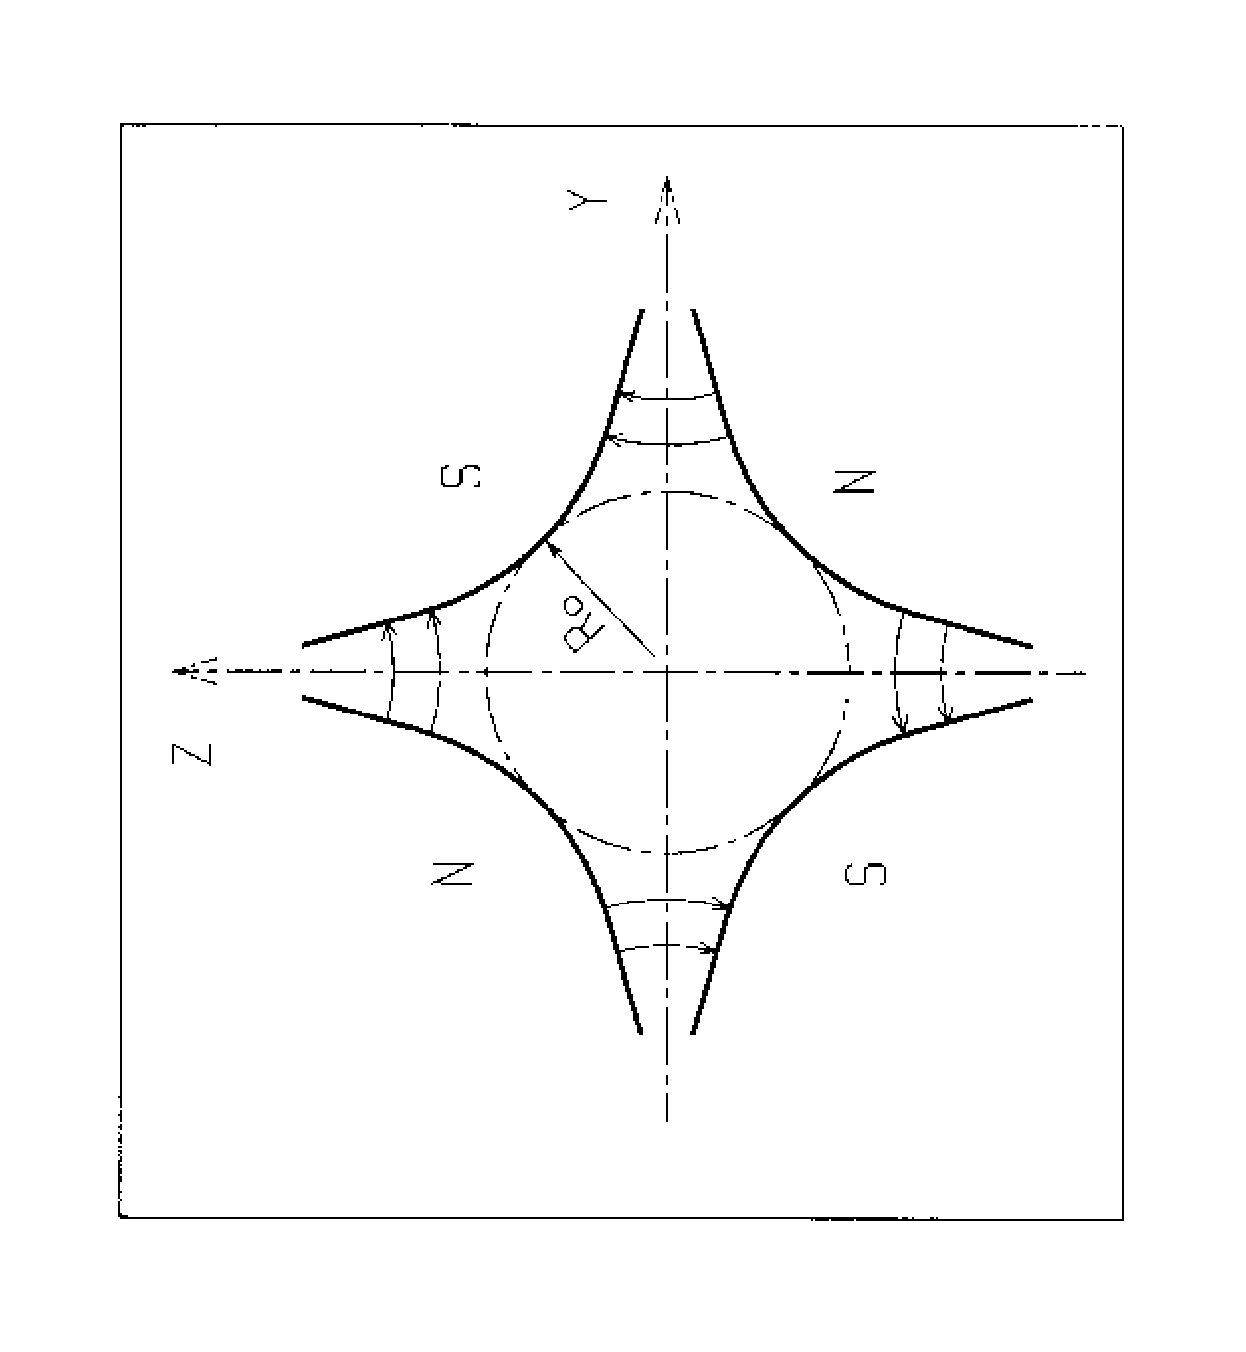
\includegraphics[height=9cm,angle=-90]{Fig26.ps}}
\unnumberedcaption{Quadrupole magnet}
\end{figure}

\vfill
%%%%%%%%%%%%%%figure%%%%%%%%%%%%%%
\begin{figure}[H]
%\vspace{11 truecm}
%%%Figure 27
\centerline{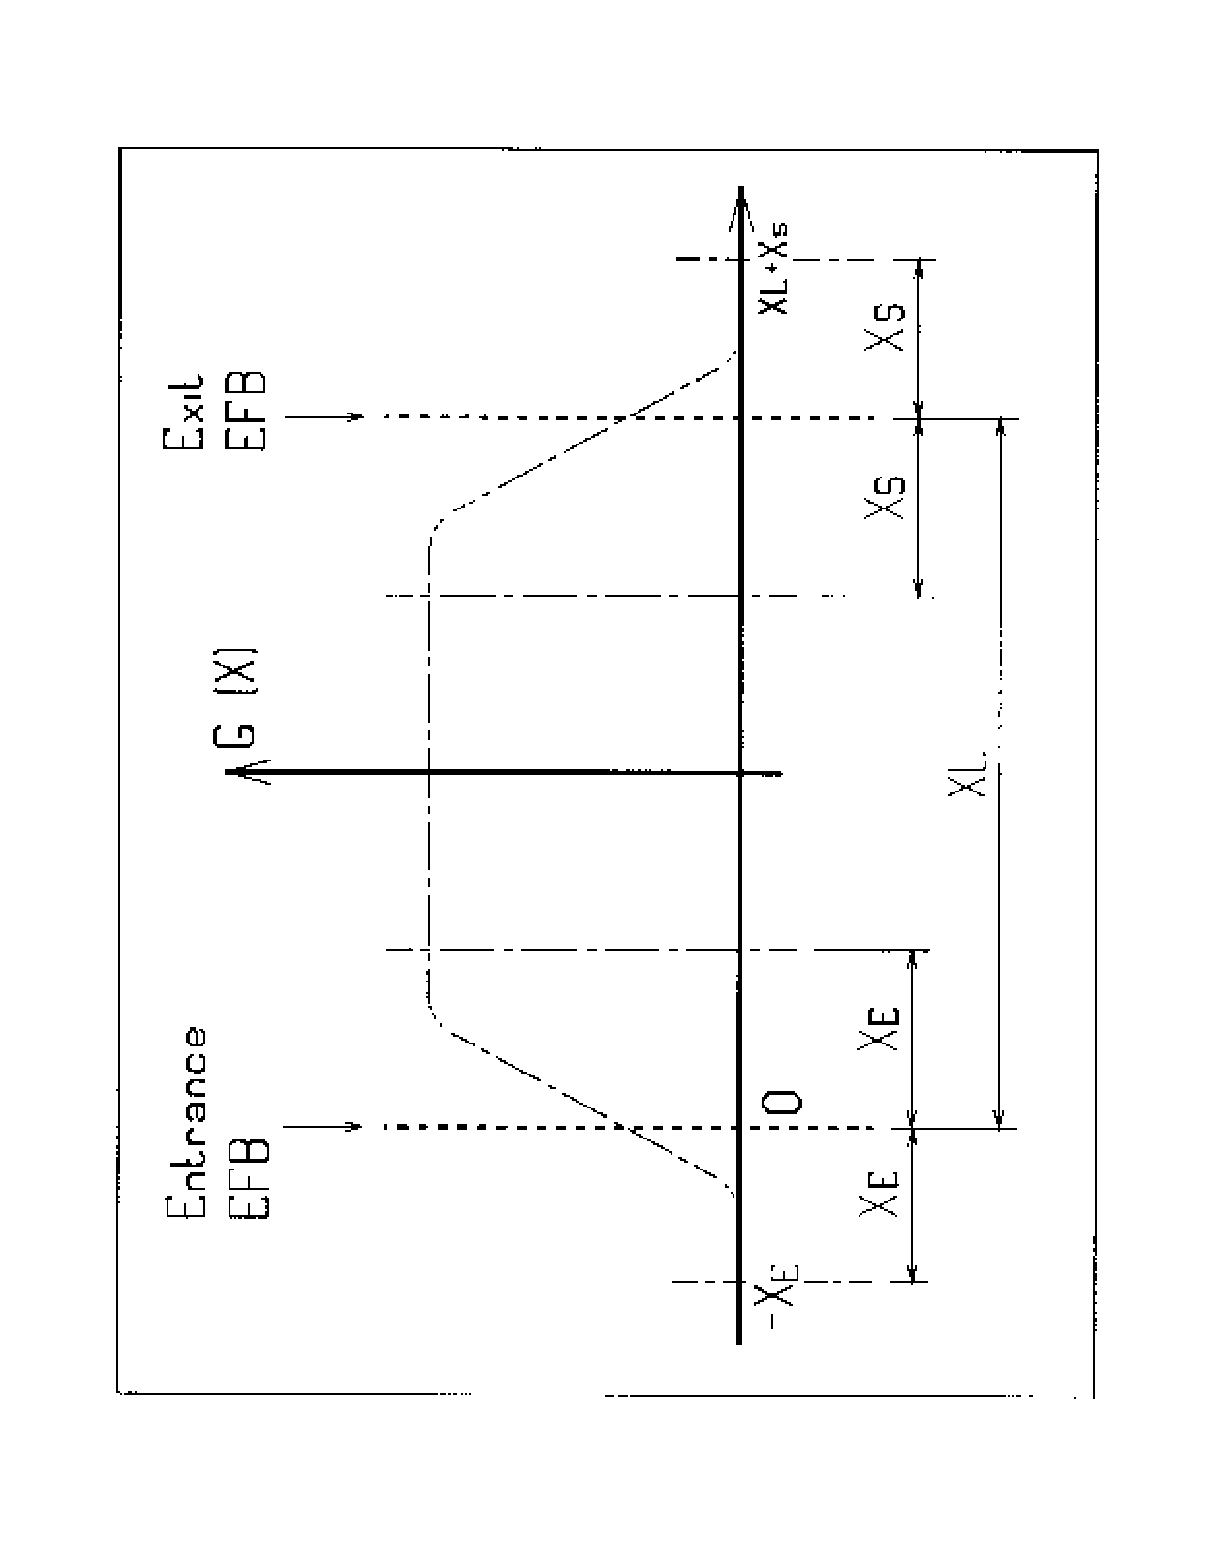
\includegraphics[height=9cm,angle=-90]{Fig27.ps}}
\unnumberedcaption[Fig27]{%
Scheme of the elements \textsl{QUADRUPO}, \textsl{SEXTUPOL},
 \textsl{OCTUPOLE}, \textsl{DECAPOLE}, 
\mbox{\textsl{DODECAPO}} \\
and \textsl{MULTIPOL}  %
\index{QUADRUPO}\index{SEXTUPOL}\index{OCTUPOLE}\index{DECAPOLE}%
\index{DODECAPO}\index{MULTIPOL} \\
$(OX)$ is the longitudinal axis of the reference frame $ (0,X,Y,Z) $  of  \zgoubi.\\
The length of the element is $ \XL $, but trajectories  are calculated 
from $ -X_E $ to $ \XL+X_S $, by means of automatic prior and further $ X_E $ and $
X_S $ translations.}
\end{figure}
\newpage

\begin{tabbing}
\mestab
\textbf{REBELOTE} \label{REBELOTE-B} \index{REBELOTE|textbf} \index{multi-particle}\index{multi-turn tracking|textbf}
		\index{acceleration}\index{synchrotron motion}
     \>      \textbf{\REBELOTETitl}   \>\>\\
 \\
 \\
 \textsl{NPASS}\index{NPASS}, \textsl{KWRIT}, $K$\textsl{[.n]}, 
           \>NPASS~: Number of runs~; \textsl{KWRIT} = 1.1 (resp. 0.0)  switches   \>arbitrary~; 0-1~; \>3*I\\
 \textsl{[IOPT]},  \>(inhibits) \textsl{FORTRAN WRITE}s to .res and to screen~; \> 0, 99~; [1[.any]]\> 2A10 \\
 \textsl{[, Label1 [, Label2]]} \> $K$  option~: \> 0-1~; 0, 22, 99 \> 2A10 \\
 \>$K=0$ : initial conditions (coordinates and spins\index{spin tracking}) \>\>\\
 \>are generated following the regular functioning \>\>\\
 \>of object definitions. If random generators are \>\>\\
 \>used (\emph{e.g.} in \textsl{MCOBJET}\index{MCOBJET}) their seeds will not be reset. \>\>\\
% \>$K=22$ :  next run will account for new parameter values in \>\>\\
% \>zgoubi.dat data list, see below. \>\>\\
 \>$K=99$ :  coordinates at end of previous pass are used as initial  \>\>\\
 \>coordinates for the next pass~; \id\ for spin components.   \>\>\\
 \>$K=99.1$ : Label1 is expected, subsequent passes will start from  \>\>\\
 \> element with Label1  down to \textsl{REBELOTE}  and so forth~; \>\>\\
 \>$K=99.2$ : Label1 and Label2 are expected~; last pass (\# NPASS+1)  \\
 \> will end at element with Label2 whereupon execution will jump to the keyword \>\>\\
 \> next to \textsl{REBELOTE}  and will be carried out down to \textsl{'END'}. \>\>\\
 \>\textsl{IOPT} is optional~: \> \> \\
 \> \textsl{IOPT = 1}~: will change the value of \textsl{NPRM} different parameters  \>\>\\
 \> in one or more of optical elements, using the data list in the next line. \>\>\\
\\
\textbf{If IOPT = 1~\footnotemark[1]}          \>   \>         \>    \\[2ex]  \label{REBEL_IOPT}
\textsl{NPRM}    \>  Number of parameters to be changed at each of the  NPASS passes. \>        \>  I  \\[1ex]
\bf \textsl{NPRM } lines with the following sequence (tells parameters concerned, and for each, its successive values)~: \\[.5ex]
\textsl{LMNT}, \textsl{KPRM}, NV*Val
         \> \textsl{LMNT}~: two possibilities, (i)~keyword number in zgoubi.dat \>  -, -, NV*dim~\footnotemark[2] \>  2*I, NV*E \\
         \>  sequence~; (ii)~\textsl{KEYWORD[, LABEL]}, i.e., keyword concerned   \>  \\
         \>  followed optionnally by is label  \>  \\
         \>  \textsl{KPRM}~: parameter number under that keyword (similar nomenclature  \>  \\
         \>   to FIT[2],  see page~\pageref{FIT-B})~; then follow the \textsl{NPASS} parameter values. \>  \\
\end{tabbing}




\vfill


\footnotetext[1]{~ \textsl{IOPT=1} is compatible with use of the \textsl{FIT[2]} \index{FIT} \index{FIT2} procedure~: \emph{e.g.},  allows successive  \textsl{FIT}s  in a single \zgou\ run, with successive sets of optical parameter values.} 

\footnotetext[2]{~  $V$ is in current \zgou\ units in the case of particle coordinates (cm, mrad). It is in MKSA units 
(m, rad) in the case of matrix coefficients.}



\newpage


\noindent  $\bullet$  Using \textbf{REBELOTE}~: An example.  \label{ExaREBELOTE} \\

\smallskip 

\noindent In this example of an energy-recovery electron recirculator based on FFAG arcs, 
 the arguments in the keyword \textsl{AUTOREF} and \textsl{CAVITE} are changed \textsl{20} times 
by \textsl{REBELOTE}, over the 21-pass recirculation process~\cite{EIC14}. The role of \textsl{AUTOREF} is
 to mimic a spreader-recombiner, \ie, re-centering the beam on the design FFAG orbit
  at the start of each one of the 11 accelerated and 10 decelerated ring turns. 
The RF voltage in \textsl{CAVITE} is set positive (accelerating, 
from 7.944~GeV to 21.16~GeV) during the first 11 passes through the optical structure, and negative 
(decerating, from 21.16 to 7.944~GeV) over the remaining 10 passes. The voltage value at each pass 
is adjusted (for an energy of 1.322~GeV per turn on average) so to compensate the energy lost by 
synchrotron radiation in the arcs.  

\bigskip

\begin{minipage}[h]{.55\linewidth}
{\tiny
\begin{verbatim}
eRHIC ENERGY RECOVERY LINAC RECIRCULATOR WITH FFAG ARCS.
 'MCOBJET'                                               1
57.36635309d3         reference rigidity (kG.cm) 
3   
2000
2 2 2 2 1 1    
-5.360667E-03   5.059706E-3  0. 0. 0.   4.619439E-01  'o'
0. 1   0.   3  
0. 1   0.   3  
0. 1.  0.     3
123456 234567 345678                                         
 'PARTICUL'                                              2
0.51099892 1.60217653e-19 1.15965218076e-3 0.0 0.0       
 'SPNTRK'                                                3
 'FAISCEAU'                                              4    
 'SRLOSS'                                                5
1   srLoss     
MULTIPOL       
1  123456      
 'SCALING'                                               6
1  1
MULTIPOL       
-1  
57.36635309 57.36635309                                  
1           11     
 'MARKER'   ARC#S_1                                      7
 'OPTIONS'                                               8
1  1
WRITE OFF                                                
 'MARKER'   MARK      CELLSTART                          9
 'DRIFT'    DRIF      HD                                10
14.547181      
 'MULTIPOL' RBEN      BD2                               11
0  .Dip        
90. 10. 0. -0.87159105   0. 0. 0. 0. 0. 0. 0. 0.
0. 0. 10.00  4.0  0.800 0.00 0.00 0.00 0.00 0. 0. 0. 0.  
4  .1455   2.2670  -.6395  1.1558  0. 0.  0.             
0. 0. 10.00  4.0  0.800 0.00 0.00 0.00 0.00 0. 0. 0. 0.  
4  .1455   2.2670  -.6395  1.1558  0. 0.  0.             
0. 0. 0. 0. 0. 0. 0. 0. 0. 0.                            
#30|90|30    Dip  BD2                                    
3   0.0E+00   4.0704703E-01  -1.5071892929E-03         
 'DRIFT'    DRIF      D                                 12
29.094362      
\end{verbatim}
\index{zgoubi.SPNPRT.Out}
}
\end{minipage}\hspace{0.03\linewidth}
\begin{minipage}[h]{.38\linewidth}
\centering
%\centerline{\includegraphics*[bbllx=20,bblly=100,bburx=567,bbury=470,width=.9\linewidth]{}}
{\tiny
\begin{verbatim}
 'MULTIPOL' RBEN      QF2                               13
0  .Dip        
110.  10.  0. 0.86286642  0. 0.0 0.0 0.0 0.0 0.0 0.0 0.0     
0. 0. 10.00  4.0  0.800 0.00 0.00 0.00 0.00 0. 0. 0. 0.  
4  .1455   2.2670  -.6395  1.1558  0. 0.  0.             
0. 0. 10.00  4.0  0.800 0.00 0.00 0.00 0.00 0. 0. 0. 0.  
4  .1455   2.2670  -.6395  1.1558  0. 0.  0.             
0. 0. 0. 0. 0. 0. 0. 0. 0. 0.                            
#30|110|30    Dip  QF2                                   
3   0.  -3.6008008661E-01  -1.8710983347E-03            
 'DRIFT'    DRIF      HD                                14
14.547181      
 'MARKER'   MARK      CELLEND                           15
----------------------------------------------------
6*138-1 additional such FD cells, simulating a 6 arc 
energy recovery ring, 138 cells per arc. 
----------------------------------------------------
 'MARKER'   ARC#E_6                                   5820    
 'OPTIONS'                                            5821
1  1
WRITE ON       
 'FAISTORE'                                           5822
zgoubi.fai     
1   
 'FAISCEAU'                                           5823
 'CAVITE'                                             5824
3   
0  0
1.322e9  1.57079632679                           
 'AUTOREF'                                            5825
4.1 
0. -5.168354E-01 4.169759E+00  5.38813280E-01            
 'FAISCEAU'                                           5826
 'REBELOTE'                                           5827
20  0.1 99 1   
4   
AUTOREF 11 -4.7493E-01 -4.1290E-01 -3.3292E-01 -2.3684E-01 
-1.26268E-01 -2.59705E-03   ... (a list of 20 values) 
AUTOREF 12  3.34619E+00  2.58215E+00  1.87157E+00  1.20916 
 5.90197E-01  1.05897E-02   ... (a list of 20 values) 
AUTOREF 13 .615682680   .692552080   .769421480  .84629088   
.923160280    1.00002970    ... (a list of 20 values) 
CAVITE  20  1.337399e9  1.33934e9   1.34012e9   1.34018e9 
... (15 more voltage values) ...  -1.30660e9  -1.309577e9 
 'SRPRNT'                                             5828
 'END'                                                5829
\end{verbatim}
}
\end{minipage}

\bigskip 


\noindent  $\bullet$ \textbf{Combining  REBELOTE and FIT}~: An example is given page \pageref{ExaFITREBELOTE}.




\newpage

\begin{tabbing}
\mestab
\textbf{RESET} \label{RESET-B} \index{RESET|textbf}  \> \textbf{\RESETTitl} \>\>\\
 \\
 \\
 \>Resets counters involved  in \textsl{CHAMBR}\index{CHAMBR}, \textsl{COLLIMA}\index{COLLIMA},  \>\>\\
 \> \textsl{HISTO}\index{HISTO} and \textsl{INTEG}\index{INTEG} procedures. \>\>\\
 \\
 \>Switches off \textsl{CHAMBR}, \textsl{MCDESINT}\index{MCDESINT}, \textsl{SCALING}\index{SCALING} and \>\>\\
 \>\textsl{SPNTRK}\index{SPNTRK} options. 
\end{tabbing}

\newpage

\begin{tabbing}
\mestab
~ ~ $ \omega^+$, $\theta$,     $R_1$, $U_1$, $U_2$  ~ ~ ~    \quad \=
 �$ B=\mathcal{F}B_0 \left(1+N \left(\frac{R-RM }{ RM} \right)      
                +B \left(\frac{R-RM}{ RM} \right)^2+G \left(\frac{R-RM }{ RM}
                \right) \right) $, ~ ~ ~ ~ ~ ~ ~     \quad \= 2*cm, 2*deg, cm   \= \kill
%%%%%%%%
\textbf{SCALING} \label{SCALING-B} \index{SCALING|textbf}  \index{acceleration}
\index{synchrotron motion}
      \>\textbf{\SCALINGTitl } \> \> \\
 \\
  \\
 \textsl{IOPT, NFAM [, PRINT]}  \>\textsl{IOPT} = 0 (inactive) or 1 (active)~; \textsl{NFAM} = number of families  
                                                                                               \>0-1, 1-45 [,-] \>I1, I2  [,A]\\
                \> to be scaled. Occurence of \textsl{PRINT} will cause printing of scaling infos  \> \> \\
                \>  in zgoubi.SCALING.out. \> \> \\
 \\
\textbf{For NF=1, NFAM :} \>repeat \textsl{NFAM} times the following sequence : \> \> \\
 \> \> \> \\
 \textsl{NAMEF [, Lbl [, Lbl]]}       \>Name of family (\emph{i.e.}, keyword of concern)~;  up to 2 labels, \> \>A10 [,A10[ \\
          \> wild card accepted, in the form \textsl{'*myLabel'} or \textsl{'myLabel*'}. \> \> ,A10]]  \\
 \\
 $NT$          \>$NT>0$~: number of timings~;   \>  -2, -1 or 1-10 \>I \\
           \>$NT=-1$~: field scaling factor updated by \textsl{CAVITE}~;   \> \> \\
           \>$NT=-2$~:  RF law in \textsl{CAVITE} is  read from external data file.  \> \> \\
 \\
 $SCL(I)$, $I=1$, $NT$ \>Scaling values (a single value if $NT=-1$~; unused if $NT=-2$)  \>relative \>NT*E\\
 \\
 $TIM(I)$, $I=1$, $NT$ \>Corresponding timings, in units of turns (1 if $NT=-1$~;   \>turn number \>NT*I \\
                       \>  unused  if      $NT=-2$).                       \>  \>  \\
% \>  Out of this range, the scaling factor is 1.
\end{tabbing} 



\newpage

\begin{tabbing}
\mestab
\textbf{SEPARA~\footnotemark[1]}         \label{SEPARA-B} \index{SEPARA|textbf}
                \> \textbf{Wien Filter - analytical simulation} \> \> \\
  \\
\\
 $IA$, $\XL$, $E$, $B$,   \>$IA=0$ : element inactive  \>0-2, m, \>I, 3*E\\
 \>$IA=1$ : horizontal separation \>V/m, T \> \\
 \>$IA=2$ : vertical separation~; \>\>\\
 \>Length of the separator~; electric field~; magnetic field.   
\end{tabbing} 

\footnotetext[1]{~ \textsl{SEPARA} must be preceded by \textsl{PARTICUL} for the definition of
mass and charge of the particles.} 
\vfill

%%%%%%%%%%%%%%figure%%%%%%%%%%%%%%
\begin{figure}[H]
%\vspace{20 truecm}
%%%Figure 28
\centerline{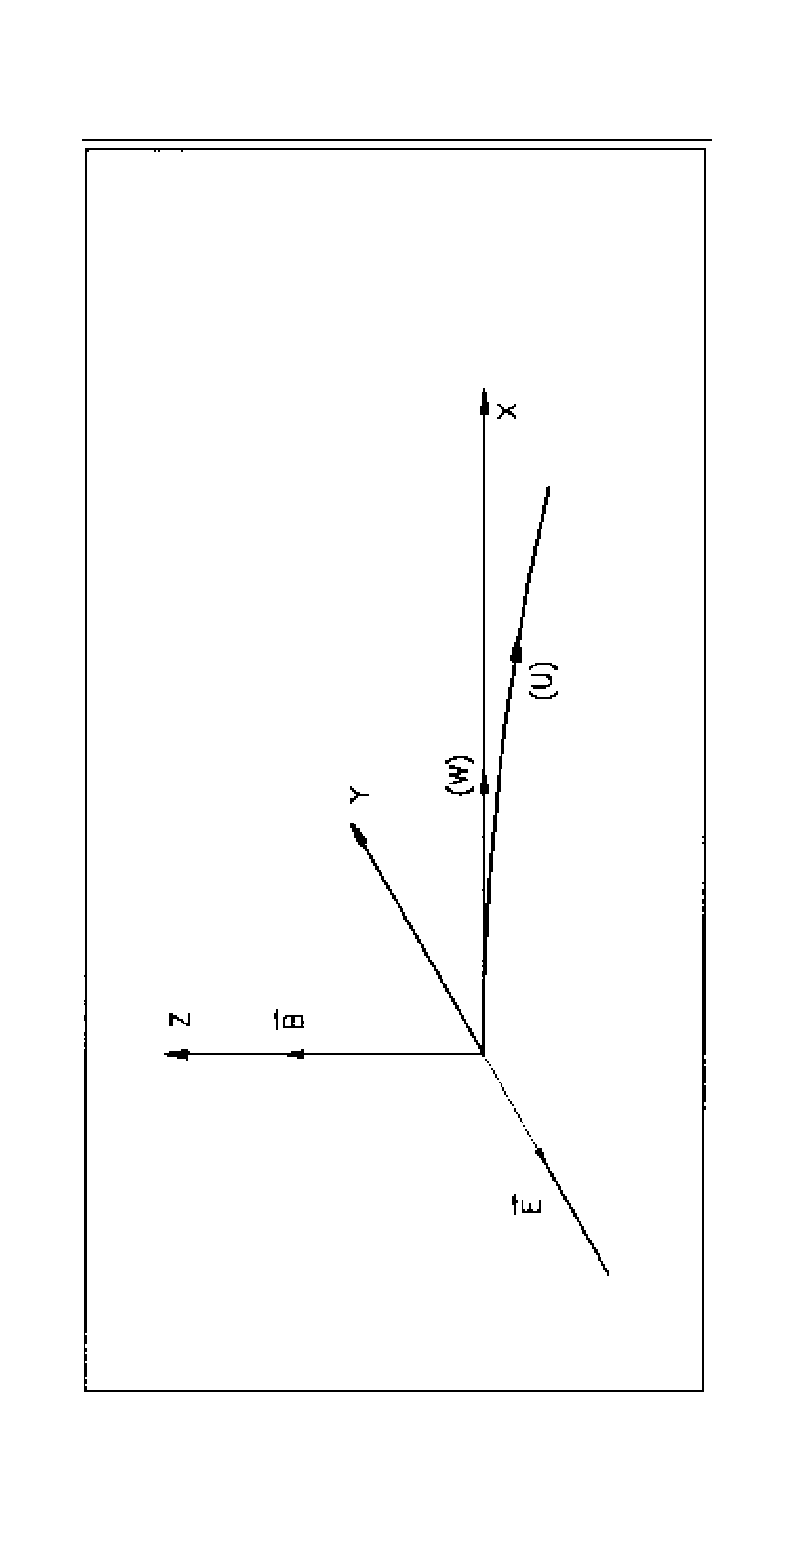
\includegraphics[height=15cm,angle=-90]{Fig28.ps}}
\medskip

\begin{center}
	\begin{minipage}[t]{13cm}
Horizontal separation between a wanted particle, $ (W)$,  
 and an unwanted particle, $ (U) $. \\
 $ (W) $ undergoes a linear motion while $ (U) $ undergoes a 
cycloidal motion.
\end{minipage}
\end{center}
 \end{figure}
\vfill


\newpage

\begin{tabbing}
$N$, $EB1$, $EB2$, $EG1$, $EG2$\quad \=
         $\IL=1,2[\times 10^n]$ : print field and coordinates along trajectories. ~ ~ ~ ~ \quad \=
             1-2, 2*cm, rad ~ ~ \quad \= \kill
%%%\mestab             
\textbf{SEXQUAD}         \label{SEXQUAD-B} \index{SEXQUAD|textbf} 
            \> \textbf{Sharp edge magnetic multipole} \> \> \\
 \> $ B_Z\mid_{ Z=0}=B_0 \left(\dfrac{N}{R_0} Y + 
      \dfrac{B}{R^2_0} Y^2 + \dfrac{G}{R^3_0} Y^3 \right)$ \> \> \\
  \\
\\
 $\IL$   \>$\IL=1,2[\times 10^n],~7$ : print coordinates, fields, etc., along trajectories \>0-2$[\times 10^n]$, 7 \>I\\
        \> in zgoubi.res ($1$),  zgoubi.plt ($2$),  zgoubi.impdev.out ($7$).       \>                   \> \\
% $\IL$   \>$\IL=1,2[\times 10^n]$ : print field and coordinates along trajectories. \>0-2$[\times 10^n]$ \>I\\
 \\
$ \XL$, $R_0 $, $B_0 $ \>Length of the element~; normalization distance~; field \>2*cm, kG 
         \>3*E\\
 \\
 $N$, $EB1$, $EB2$, $EG1$, $EG2$ \>Coefficients for the calculation of B. \>5*no dim. \>5*E\\
 \>if $Y>0$ : $B=EB1$ and $G=EG1$~; \>\>\\
 \>if $Y<0$ : $B=EB2$ and $G=EG2$. \>\>\\
 \\
 \textsl{XPAS}          \>Integration step  \>cm \>E \\
 \\
 \textsl{KPOS}, \textsl{XCE},    \textsl{YCE, ALE}     \>\textsl{KPOS}=1 : element aligned, 2 : misaligned~; shifts, tilt. 
           \>1-2, 2*cm, rad \>I, 3*E \\
\end{tabbing}


\newpage

\begin{tabbing}
$N$, $EB1$, $EB2$, $EG1$, $EG2$\quad \=
         $\IL=1,2[\times 10^n]$ : print field and coordinates along trajectories. ~ ~  ~ ~ \quad \=
             1-2, 2*cm, rad ~ ~ \quad \= \kill
%%%\mestab             
\textbf{SEXTUPOL }           \label{SEXTUPOL-B} \index{SEXTUPOL|textbf}
          \> \textbf{Sextupole Magnet }  \> \> \\
 \\
 $\IL$   \>$\IL=1,2[\times 10^n],~7$ : print coordinates, fields, etc., along trajectories \>0-2$[\times 10^n]$, 7 \>I\\
        \> in zgoubi.res ($1$),  zgoubi.plt ($2$),  zgoubi.impdev.out ($7$).       \>                   \> \\
% $\IL$        \>$\IL=1,2[\times 10^n]$ : print field and coordinates along trajectories. \>0-2$[\times 10^n]$ \>I \\
 \\
 $\XL$, $ R_0$, $B_0 $ \>Length~; radius and field at pole tip of the element \>2*cm, kG \>3*E \\
 \\
 \>\textbf{Entrance face :} \>\>\\
$ X_E$, $\lambda_E $    \>Integration zone~; fringe field \>2*cm \>2*E \\
 \>extent ($ \lambda_E=0 $ for sharp edge) \>\>\\
 \\
 \textsl{NCE}, $ C_0-C_5 $ \>\textsl{NCE} = unused \>any, 6* \>I, 6*E \\
 \>$ C_0-C_5 $ = Fringe field coefficients such that  \>no dim. \> \\
 \>$ G(s)=G_0/(1+ \exp  P(s)), $ with $ G_0=B_0/R^2_0 $ \>\>\\
 \>and $ P(s) = \sum^ 5_{i=0}C_i(s/\lambda )^i $ \>\>\\
 \\
 \>\textbf{Exit face :} \>\>\\
$ X_S$, $\lambda_ S $    \>Parameters for the exit fringe field~; see entrance \>2*cm \>2*E \\
 \\
 \textsl{NCS}, $ C_0-C_5 $ \> \>0-6, 6*no dim. \>I, 6*E \\
 \\
 \textsl{XPAS}          \>Integration step  \>cm \>E \\
 \\
 \textsl{KPOS}, \textsl{XCE},    \textsl{YCE, ALE}      \>\textsl{KPOS}=1 : element aligned, 2 : misaligned~; shifts, tilt. 
           \>1-2, 2*cm, rad \>I, 3*E \\
\end{tabbing}

%\newpage
%%%%%%%%%%%%%%figure%%%%%%%%%%%%%%
\begin{figure}[H]
%\vspace{12 truecm}
%%%Figure 29
\vfill
\centerline{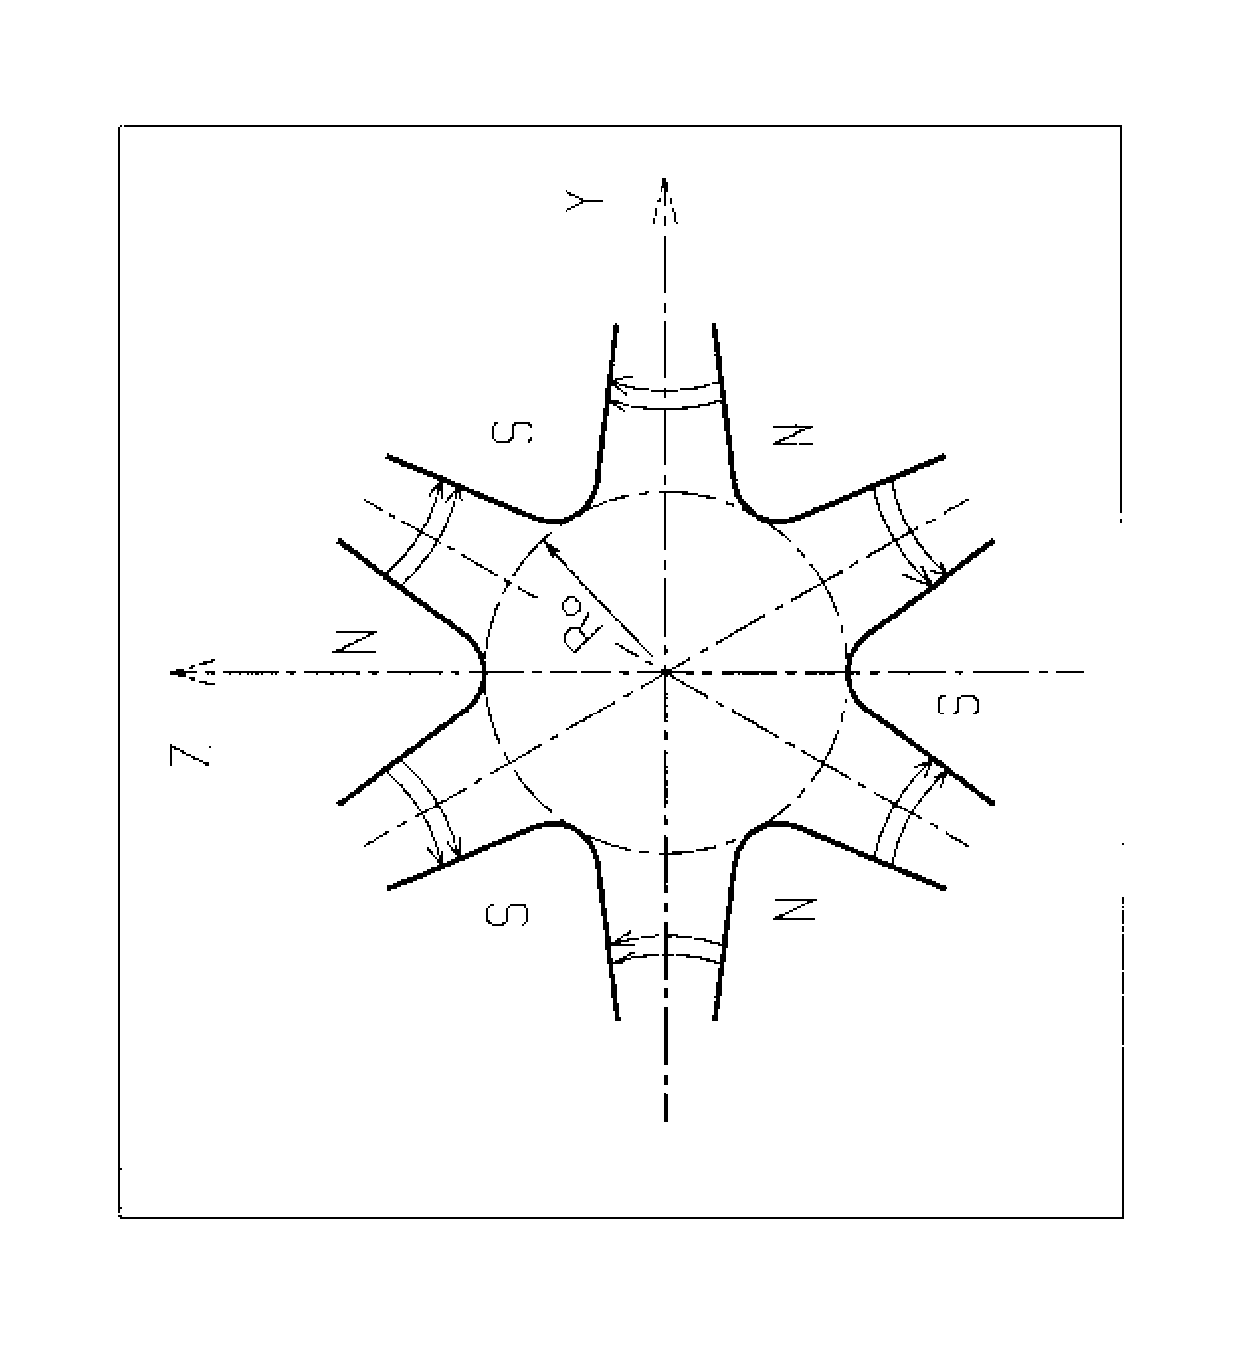
\includegraphics[height=10cm,angle=-90]{Fig29.ps}}
\unnumberedcaption{Sextupole magnet}
\vfill
\end{figure}


\newpage

\begin{tabbing}
$N$, $EB1$, $EB2$, $EG1$, $EG2$\quad \=
         $\IL=1,2[\times 10^n]$ : print field and coordinates along trajectories. ~ ~  ~ ~ \quad \=
             1-2, 2*cm, rad ~ ~ \quad \quad \= \kill
%%%\mestab             
 \textbf{SOLENOID}        \label{SOLENOID-B} \index{SOLENOID|textbf}
     \> \textbf{\SOLENOIDTitl} \> \> \\
 \\
 \\
 $\IL$   \>$\IL=1,2[\times 10^n],~7$ : print coordinates, fields, etc., along trajectories \>0-2$[\times 10^n]$, 7 \>I\\
        \> in zgoubi.res ($1$),  zgoubi.plt ($2$),  zgoubi.impdev.out ($7$).       \>                   \> \\
% $\IL$  \> $\IL=1,2[\times 10^n]$ : print field and coordinates along trajectories. \>0-2$[\times 10^n]$\>I\\
 \>\>\>\\
 $\XL$, $R_0 $, $B_0 $  \textsl{[, MODL]}   \>Length~; radius~; asymptotic field (=$ \mu_0 NI/\XL $)~; \textsl{MODL=1}~: default,  \>2*cm, kG [, no dim.] \>3*E \\
     \>   $r$-extrapolation from on-axis field model, \textsl{MODL=2}~: elliptic    \> \> \\
     \>   integrals method      \> \> \\
 \\
$ X_E$, $X_S $        \>Entrance and exit integration zones \>2*cm\>2*E\\
 \\
 \textsl{XPAS}          \>Integration step  \>cm \>E \\
 \\
 \textsl{KPOS}, \textsl{XCE},   \textsl{YCE, ALE}      \>\textsl{KPOS}=1 : element aligned, 2 : misaligned~; shifts, tilt. 
           \>1-2, 2*cm, rad \>I, 3*E \\
\end{tabbing}
 
\vfill
%%%%%%%%%%%%%%figure%%%%%%%%%%%%%%
\begin{figure}[H]
%\vspace{14 truecm}
%%%Figure 30
\centerline{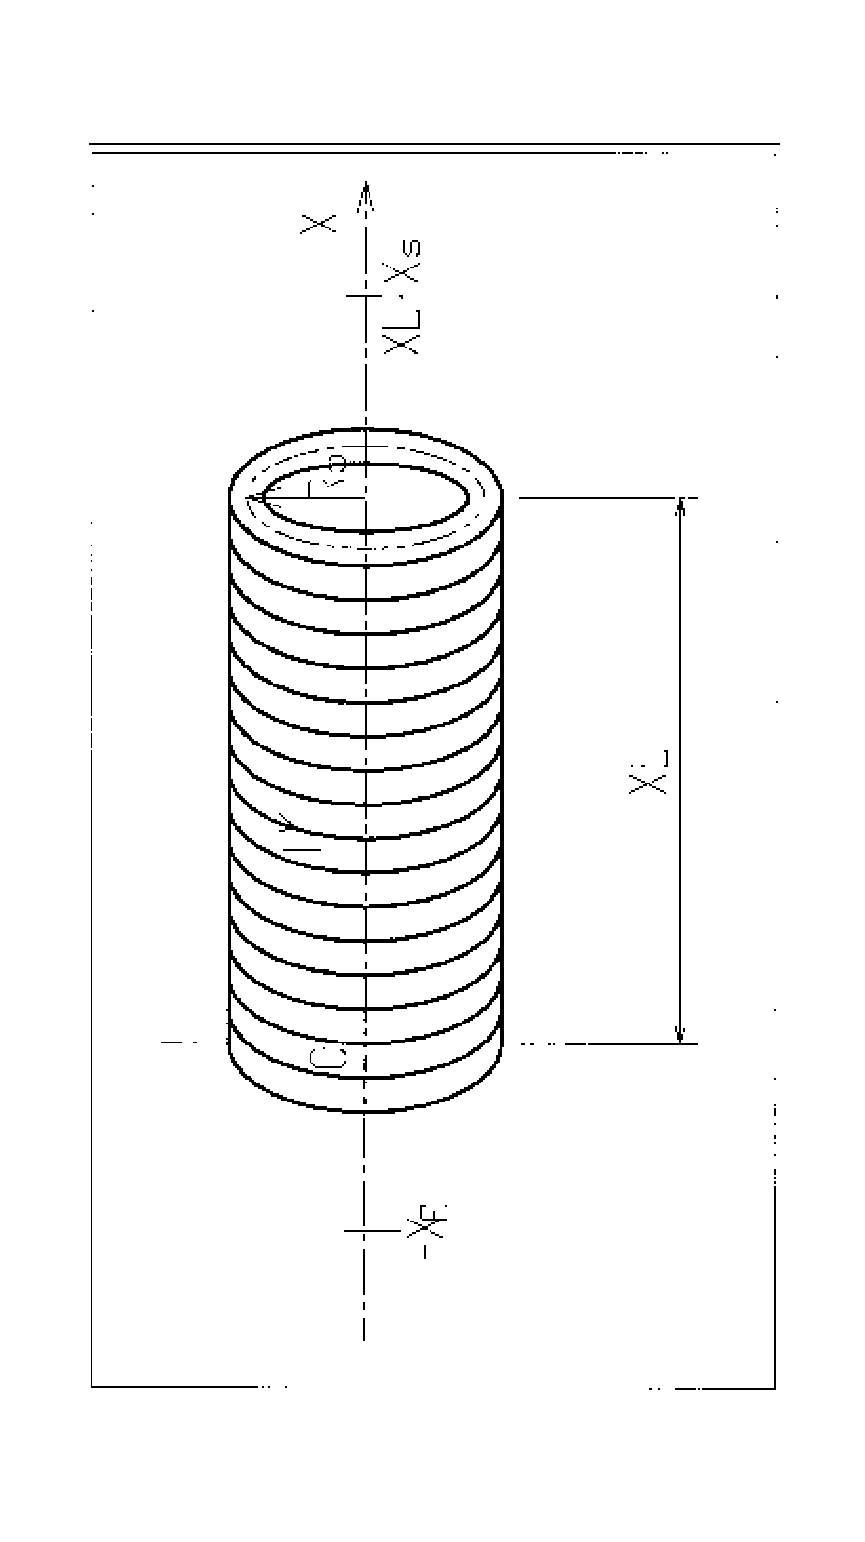
\includegraphics[height=15cm,angle=-90]{Fig30.ps}}
\end{figure}
\vfill





\newpage

\begin{tabbing}
\mestab
 \textbf{SPACECHARG}        \label{SPACECHARG-B} \index{SPACECHARG|textbf}
     \> \textbf{\SPACECHARGTitl} \> \> \\
 \\
\textsl{LMNT, model [, PRINT]} \> \textsl{LMNT} = 'all',  'none', or keyword~; model~: 'KV', 'Gaussian'~;    \> -, - [,-] \> 2*A [,A] \\
   \> [optional : print out to zgoubi.SPACECHARG.out].  \> \> \\
\\
$\lambda$ \> Linear charge density   \> $C/m$ \>  E\\
\\
  \end{tabbing}





\newpage

\begin{tabbing}
$N$, $EB1$, $EB2$, $EG1$, $EG2$\quad \=
         $\IL=1,2[\times 10^n]$ : print field and coordinates along trajectories. ~ ~  ~ ~ \quad \=
             1-2, 2*cm, rad ~ ~ \quad \= \kill
%%%\mestab             
 \textbf{SPINR}        \label{SPINR-B} \index{SPINR|textbf}
     \> \textbf{\SPINRTitl} \> \> \\
% \\
% \\
% $\Theta_x$, $\Phi_X$      \>Angles that define the spin precession axis. \>2*rad \>2*E \\
% \\
% $\mu$     \>Spin precession  angle. \>rad \>E \\
% \\
 \\
 \\
 \textsl{IOPT}       \> Option    \>0-2 \>I \\
 \\
\textbf{If IOPT=0}  \>Element inactive \>\>\\
\\
$ X$, $X $        \> Unused \> 2*unused\> 2*E\\
  \\
\textbf{If IOPT=1}  \> \bf Axis and spin precession angle values.\\
 \\
 $\mu$, $\phi$ \> Angle (in $(X,Y)$ plane) between the X-axis and the spin precession \> deg, deg \> 2*E \\
                \>  axis~; spin precession angle around that axis. \>  \>  \\
\\
\textbf{If IOPT=2}  \>\bf Given the spin precession axis direction, $\mu$, in the horizontal plane, the spin precession \\
   \> \bf angle follows a function of the Lorentz factor~: $\phi(\gamma) = \left(\dfrac{B}{B_0}\right)^2 * \left( C_0 + \dfrac{C_1}{\gamma} + \dfrac{C_2}{\gamma^2}  + \dfrac{C_3}{\gamma^3} \right) $  \\
 \\
$\mu$, $B$, $B_0$,  \> Angle  (in $(X,Y)$ plane)  between the X-axis and the spin  \> deg.; 6*no dim \> 7*E \\
$C_0$, $C_1$, $C_2$, $C_3$  \> precession axis~; six coefficients that define the spin precession \>  \>  \\
  \> around that axis. \>  \>  \\
\end{tabbing}
 





\newpage

\begin{tabbing}
\mestab
% \textbf{SPNPRT}        \label{SPNPRT-B} \index{SPNPRT}
%     \> \textbf{Print spin\index{spin tracking} coordinates} \> \> \\
%  \\
%\\
% \> Print spin coordinates at the location where this \\
% \> keyword is introduced in the structure. \\[60pt]
 \textbf{SPNPRNL}        \label{SPNPRNL-B} \index{SPNPRNL|textbf}
     \> \textbf{Store spin coordinates in file \textsl{FNAME}} \> \> \\
 \\
 \\
\textsl{FNAME~~\footnotemark[1]} \> Name of storage file (\emph{e.g.}, zgoubi.spn\index{zgoubi.spn}) \>\> A80 \\[60pt]
%
%
 \textbf{SPNSTORE}        \label{SPNSTORE-B} \index{SPNSTORE|textbf}
     \> \textbf{Store spin coordinates every $IP$ other pass} \> \> \\
\\
 \\
 \textsl{FNAME}~~\footnotemark[1]
       \>Name of storage file (\emph{e.g.},~zgoubi.spn) [~; label(s) of the element(s)  \> \>A80\\ %%
{[,}\textsl{\LABEL(s)}{]}~~\footnotemark[2]  \index{LABEL@{\LABEL}}   \>  at the exit of which the store occurs (10 labels 
       maximum)]. \> \> [, 10*A10] \\
       \\
 $IP$ 	\> Store every $IP$ other pass (when using \textsl{REBELOTE}\index{REBELOTE} \> \>I\\
 \> with \textsl{NPASS}\index{NPASS} $\geq IP-1$).  \\[60pt]
%
%
 \textbf{SPNPRT [PRINT]}        \label{SPNPRT-B} \index{SPNPRT|textbf}
     \> \textbf{Print spin coordinates} \>  \\
\\
 \> Print spin coordinates in zgoubi.res, at the location where this  keyword is introduced  \\
 \> in the structure. \\
 \> The first label, '\textsl{PRINT}', is optional, if it appears, then local data are stored in  the file  \\
 \> zgoubi.SPNPRT.Out. That file is open at the first occurence of \textsl{SPNPRT} and left open  \\
 \> until \zgou\ execution is completed. 
\\
  \end{tabbing}
 
\begin{alltt}
\footnotetext[1]{ \textsl{FNAME} = 'none' will inhibit printing.}
\footnotetext[2]{ If first \textsl{\LABEL} = 'none' then  printing will be inhibited.}
\end{alltt}



\newpage

\begin{tabbing}
\mestab
 \textbf{SPNTRK~\footnotemark[1]}        \label{SPNTRK-B} \index{SPNTRK|textbf}\index{spin tracking}
     \> \textbf{Spin tracking} \> \> \\
 \\
\textsl{KSO [.KSO2]} \> \textsl{KSO=0}~: spin tracking [switched] off~\footnotemark[2]~; \textsl{KSO=~-1}~: spin  tracking  \> -1 or 0 or  \> I \\
             \>   resumes. Otherwise~: as stated below.                                        \> 1-3 0r 4[.1] or 5 \>  \\
\\
\textbf{If KSO = 1 --  3} \> \textsl{KSO} = 1 (respectively 2, 3) : all particles \\
      \> have their spin automatically set to (1,0,0), \\
      \> longitudinal [respectively (0,1,0), horizontal \\
      \> and (0,0,1), vertical] \\
\\
\textbf{If KSO = 4}    \>  Repeat \IMAX\ times (corresponding to the \IMAX \\
      \> particles in `\textsl{OBJET}') the following sequence : \\
\\
$S_X$, $S_Y$, $S_Z$   \> $X$, $Y$ and $Z$ initial components of the initial spin. \> 3*no dim. \> 3*E \\
\\
\textbf{If KSO = 4.1}    \>      \>  \\
\\
$S_X$, $S_Y$, $S_Z$   \> $X$, $Y$ and $Z$ components of the initial spins. \> 3*no dim. \> 3*E \\
                     \> These  will be assigned to all particles.   \>  \> \\
\\
\textbf{If KSO = 5} \> Random distribution in a cone (see figure)\\
      \> Enter the following two sequences : \\
$TO$, $PO$, $A$, $\delta A$ \> Angles of average polarization : \> 4*rad \> 4*E \\
        \> $A$ = angle of the cone~; $\delta A$ = standard deviation \\
        \> of distribution around $A$ \\
\\
$IR$ \> Random sequence seed  \> $\losim 10^6$  \> I              
  \end{tabbing}
  
\footnotetext[1]{~ \textsl{SPNTRK} must be preceded by \textsl{PARTICUL} for
 the definition of $G$ and mass.}

\footnotetext[2]{~ Spin tracking can be switched off at any location in zgoubi.dat data list using \textsl{KSO=0}, 
and further away resumed using \textsl{KSO=~-1}.}




\newpage


\begin{tabbing}
\mestab
 \textbf{SRLOSS}        \label{SRLOSS-B} \index{SRLOSS|textbf}
     \> \textbf{\SRLOSSTitl}\index{synchrotron radiation loss} \> \> \\
 \\
\textsl{KSR[.i]}     \> On/off switch~; $i=1$ for info output  into \texttt{zgoubi.SRLOSS.Out}       \> $0~or~1[.1]$  \> 2*I \\
\\
\textsl{STR1 [, STR2]} \> \textsl{STR1 = 'ALL'} or \textsl{'all'} or a particular magnet KEYWORD.  \> \> 2*A \\
                    \> Optional~: \textsl{STR2 = 'scale'} will scale fields following energy loss.              \>  \\
 \\
\textsl{Option}, seed \>  Option~: 0 / no effect, 1 / SR causes dp only,   \> $1-3$,  $>10^5$ \> 2*I \\
                \>  2 / SR causes dp and angle kick (not installed).  \> \\

  \end{tabbing}
  


\newpage

\begin{tabbing}
\mestab
 \textbf{SRPRNT}        \label{SRPRNT-B} \index{SRPRNT|textbf}\index{SRLOSS}
     \> \textbf{\SRPRNTTitl}   ~~ into zgoubi.res

\end{tabbing}



\newpage

\begin{tabbing}
\mestab
 \textbf{SYNRAD}        \label{SYNRAD-B} \index{SYNRAD|textbf}
     \> \textbf{\SYNRADTitl}\index{synchrotron radiation spectra} \> \> \\
 \\
\textsl{KSR} \> Switch \> 0-2 \> I \\
   \> 0 : inhibit SR calculations \> \> \\
   \> 1 : start \> \> \\
   \> 2 : stop \> \> \\
\\
\textbf{If KSR = 0} \> \> \> \\
\\
$D1$, $D2$, $D3$      \> Dummies \> \> 3*E \\
 \\
\textbf{If KSR = 1}   \> \> \> \\
\\
$X0$, $Y0$, $Z0$ \> Observer position in frame of magnet next to \textsl{SYNRAD} \> 3*m \> 3*E \\
\\
\textbf{If KSR = 2} \> \> \> \\
\\
 $\nu_1$, $\nu_2$, $N$   \> Frequency range and sampling \> 2*eV, no dim. \> 2*E, I 
  \end{tabbing}
  



\newpage

\begin{tabbing}
\mestab
 \textbf{SYSTEM}        \label{SYSTEM-B} \index{SYSTEM|textbf}
     \> \textbf{\SYSTEMTitl}\index{system call} \> \> \\
 \\
\textsl{NCMD} \> The number of calls to follow.  \> $\geq 0$ \> I \\
\\
\\
\textsl{NCMD lines follow, one command per line. }
 \\
  \end{tabbing}
  


\newpage

\noindent  $\bullet$  \textbf{SYSTEM}~: An example (an additional example can be found page~\pageref{ExaFITREBELOTE}) \\

\label{ExaSYSTEM}

\smallskip 

\noindent The first occurence of the command (top region in the data list below) 
allows establishing links from remote folders to the current one (the one in which \zgou\ 
is presently run). These folders happen to contain  files appearing in the \textsl{SCALING} command, 
as well as OPERA field maps of the siberian snakes used in subsequent \textsl{TOSCA} commands.

The second occurence of the command (bottom region in the data list below) 
allows saving  zgoubi.res output file as resulting from the \zgou\ run, under a different name. 

~

%\hspace{-0.05\linewidth}
\begin{minipage}{.48\linewidth}
\tiny  %\scriptsize
\begin{verbatim}
AGS, polarized protons. 2 snakes. t = 145 ms.
'GETFITVAL'       
fitVals.data
'OBJET'     LBL_OBJfit                                      
7069.3668040036146
5
.01 .01 .01 .01 0. .0001    
  0.  0.  0.  0.  0.  1.    'o'       
'FAISCEAU'
'SYSTEM'
 2
ln -sf /rap/lattice_tools/zgoubi/AgsZgoubiModel/snakeFieldMaps/TOSC3D/Csnk3D .
ln -sf /rap/lattice_tools/zgoubi/AgsZgoubiModel/snakeFieldMaps/TOSC3D/Wsnk3D . 
'SCALING'   LBL_SCLfit
1   21
AGSMM *AF *BF *CF  !# of params 2Bchanged. dB0 (FIT#3) dB1 (FIT#4)      dB2     
-1                  3                      13  3E-20   14 -1.473595E-03 15  8.01942
1.00000000     ! (FIT #6)
1
AGSMM *AD *BD *CD  !# of params 2Bchanged. dB0 (FIT#9) dB1 (FIT#10)     dB2   
-1                  3                      13  9E-20   14 -1.011857E-03 15 -1.70597
1.000000      ! (FIT#12)
1
AGSQUAD  QH_*   !# of params 2Bchanged.      (FIT#15)
-1               1                       15   0.0   
1.000000
1
AGSQUAD  QV_*  QP_*      !# of params 2Bchanged.       (FIT#15)
-1                        1                       15    0.0  
1.000000
1
MULTIPOL   QJUMP_*
-1
7.06936680E+00
1
MULTIPOL   SXH_*
-1
7.06936680E+00
1
MULTIPOL   SXV_*
-1
7.06936680E+00
1
AGSMM MM_F08CD MM_F09BF MM_G02BF MM_G03CD MM_G16AD MM_G17CF  ! blw1 / G9  bump
-1          1        22    -.0762e-99                ! Amp.  (FIT #31)
1.0
1
AGSMM MM_H04CD MM_H05AF MM_H18CF MM_H19BD MM_I12BD MM_I13CF  ! blw1 / H11 bump
-1          1        22    -.06093e-99               ! Amp.  (FIT #35)
1.0
1
MULTIPOL COH1
1.10
./Csnk3D/Hlx68.2_Sol42.3/CHREF_+_dipolCORR.scal
1 4
MULTIPOL COV1
1.10
./Csnk3D/Hlx68.2_Sol42.3/CHREF_+_dipolCORR.scal
1 5
MULTIPOL COH2
1.10
./Csnk3D/Hlx68.2_Sol42.3/CHREF_+_dipolCORR.scal
1 6
MULTIPOL COV2
1.10
./Csnk3D/Hlx68.2_Sol42.3/CHREF_+_dipolCORR.scal
1 7
MULTIPOL WOH1
1.10
./Csnk3D/Hlx68.2_Sol42.3/CHREF_+_dipolCORR.scal_51.8_0.0
1 4
MULTIPOL WOV1
1.10
./Csnk3D/Hlx68.2_Sol42.3/CHREF_+_dipolCORR.scal_51.8_0.0
1 5
MULTIPOL WOH2
1.10
./Csnk3D/Hlx68.2_Sol42.3/CHREF_+_dipolCORR.scal_51.8_0.0
1 6
MULTIPOL WOV2
1.10
./Csnk3D/Hlx68.2_Sol42.3/CHREF_+_dipolCORR.scal_51.8_0.0
1 7
CHANGREF WSNKE
1.12
./Csnk3D/Hlx68.2_Sol42.3/CHREF_+_dipolCORR.scal_51.8_0.0
1 1  1 3
CHANGREF WSNKO
1.12
./Csnk3D/Hlx68.2_Sol42.3/CHREF_+_dipolCORR.scal_51.8_0.0
1 1  1 2
CHANGREF CSNKE
1.12
./Csnk3D/Hlx68.2_Sol42.3/CHREF_+_dipolCORR.scal
1 1  1 3
CHANGREF CSNKO
1.12
./Csnk3D/Hlx68.2_Sol42.3/CHREF_+_dipolCORR.scal
1 1  1 2
\end{verbatim}
\end{minipage}\hspace{.05\linewidth}
\begin{minipage}{.38\linewidth}
\tiny  %\scriptsize
\begin{verbatim}
'MARKER'   #Start
'OPTIONS'
1 1  ! options
WRITE OFF
'AGSMM'  MM_A01BF
0
3 0 0   0.00000E+00  1.00000E+00  1.00000E+00  1.0
2.1  1 0.  1 0.
0. 0. 10.00  4.0  0.800 0.00 0.00 0.00 0.00 0. 0. 0. 0.
4  .1455   2.2670  -.6395  1.1558  0. 0.  0.
0. 0. 10.00  4.0  0.800 0.00 0.00 0.00 0.00 0. 0. 0. 0.
4  .1455   2.2670  -.6395  1.1558  0. 0.  0.
0. 0. 0. 0. 0. 0. 0. 0. 0. 0.
3.0  Dip MM_A01BF
4 0. 0. 0. 0. 0.
[......]
'TOSCA'
0  0
1.e-3 100. 100. 100.
HEADER_4 csnake
281 29 29  15.2 .682 .423
./Csnk3D/Hlx68.2_Sol42.3/b_table_for_Helix_3T.tab
./Csnk3D/Hlx68.2_Sol42.3/b_table_for_Solen.tab
0 0 0 0
2
.1
2  0.  .00  0.  0.
[......]
'TOSCA'
0  0
1.e-3 100. 100. 100.
HEADER_4 csnake
281 29 29  15.2 .518 1.e-30
./Csnk3D/Hlx68.2_Sol42.3/b_table_for_Helix_3T.tab_2
./Csnk3D/Hlx68.2_Sol42.3/b_table_for_Solen.tab_2
0 0 0 0
2
.1
2  0.  .00  0.  0.
[......]
'MARKER'   #End
'FAISCEAU'
'OPTIONS'
1 1  ! options
WRITE ON
'FAISCEAU'
'MATRIX'
1   11                     
'SYSTEM'
1
cp zgoubi.res zgoubi.res_save
'END'   
\end{verbatim}

\end{minipage}




\newpage


\begin{tabbing}
\mestab
 \textbf{TOSCA}        \label{TOSCA-B} \index{TOSCA|textbf}
     \> \textbf{\TOSCATitl} \> \> 
 \\
 \\
 $\IC$, $\IL$      \>$\IC=1,2$ : print  the map \>0-2; 0-2$[\times 10^n]$, 7 \>2*I\\
    \>$\IL=1,2[\times 10^n],~7$ : print coordinates, fields, etc., along trajectories \> \>   \\
        \> in zgoubi.res ($1$),  zgoubi.plt ($2$),  zgoubi.impdev.out ($7$).       \>                   \> \\
 \\
 \textsl{BNORM, XN,YN, ZN}      \> Field and  X-,Y-,Z-coordinate normalization coefficients. \> 4*UnitConv. \> 4*E \\
        \> Convert values  as read from map file, to kG and cm or rad. \\
 \\
 \textsl{TITL}        \>Title. Include ``FLIP'' to get field map X-flipped. Include \> \>A80 \\
                      \>``HEADER n'' in case \textsl{FNAME} starts with $n\geq1$ header lines.  \> \> \\
 \\
 $IX$, $IY$, $IZ,$~\footnotemark[1]     \>Number of nodes of the mesh in the $X$, $Y$    \>$\leq$\textsl{MXX}, $\leq$\textsl{MXY}, \>3*I, I[.I  \\
\textsl{MOD[.MOD2 [, a(i),i=} \> and $Z$ directions, $IZ=1$ for a 2-D map~; \textsl{MOD} \> $\leq$\textsl{IZ}, [0-22.1-9], - \> [, MOD2*E]]\\
  \textsl{1,MOD2]]}    \> and \textsl{MOD2} : field map style, see table next page. \> \> \\
 \\
Next NF lines :   \> Map file name(s), one line per name.   \> \>A80 \\
\textsl{FNAME}~\footnotemark[3] \> If \textsl{MOD}=0 : $NF = 1+ [IZ/2]$, the $NF$ 2-D maps are for $0 \leq Z \leq Z_{max}$, \\
      \> they are symmetrized with respect to the $Z(1)=0$ plane.\\
       \> If \textsl{MOD}=1 : $NF = IZ$, no symmetry assumed~; $Z(1) = Z_{max}$,  \\ 
       \> $Z(1+ [IZ/2])=0$ and $Z(NF) = -Z_{max}$ .\\ 
       \> If \textsl{MOD}=12 : a single \textsl{FNAME}  file contains the all 3-D volume.  \\ 
       \> \textsl{MOD=15, 20-22}, etc.~: see table next page.  \> \> \\
 \\
$ID$, $A$, $B$, $C$ {[}, $A'$, $B'$, $C'$,\>Integration boundary. Ineffective when $ID=0$.     \>$\geq -1$,  cm, \>I,3*E  \\
$A''$, etc., if $\left. ID\geq 2\right]$ \>$ID=$ -1, 1 or $\geq 2$ : as for \textsl{CARTEMES}\>2*no dim. [,\id]\>[,3*E,etc.]\\
 \\
 \textsl{IORDRE}     \>If $IZ=1$ : 2, 25 or 4 as in \textsl{CARTEMES\index{CARTEMES}}~; unused if $IZ \not =1$.  \>2, 25 or 4 \>I\\
 \\
 \textsl{XPAS}          \>Integration step  \>cm \>E \\
 \\
 \textbf{If Cartesian mesh (see MOD) : } \\
 \textsl{KPOS, XCE, YCE, ALE}    \>\textsl{KPOS}=1 : element aligned, 2 : misaligned~; shifts, tilt  \>1-2, 2*cm, rad \>I, 3*E \\
 \textbf{If polar mesh : } \\
 \textsl{KPOS}    \>as for \textsl{POLARMES}. Normally 2.    \>1-2  \>I \\
 \textbf{If KPOS = 2 :} \> \> \> \\
 $RE$, $TE$, $RS$, $TS$ \> \> cm, rad, cm, rad \> 4*E \\
 \end{tabbing}


\begin{alltt}
\footnotetext[1]{\textsl{MXX, MXY, IZ} may be changed, they are stated in the include file \texttt{PARIZ.H}. }
\footnotetext[2]{\textrm{Case of 2-D field maps : Each file \textsl{FNAME(K)} contains the field specific to elevation \(Z(K)\) and must be formatted according to the following \textsl{FORTRAN} read sequence (that usually fits \textsl{TOSCA} code \textsl{OUTPUTS} - details and possible updates are to be found in the source  file \texttt{'fmapw.f'}) :} 
{\tiny
   DO JF = 1, NF
     OPEN (UNIT = NL, FILE = FNAME(JF), STATUS = `OLD' [,FORM='UNFORMATTED'])
     DO J = 1,  JY ;       DO I = 1, IX
         READ(NL,*) Y(J), Z(JF), X(I), BY(J,I), BZ(J,I), BX(J,I)    \hfill      {\footnotesize node coordinates, field components at node}
     ENDDO ;     ENDDO
     NL = NL + 1
   ENDDO} 
BX and BY are assumed  zero at all nodes of the 2-D mesh, regardless of BX(J,1,I), BY(J,1,I) values. 
\textrm{Case of 3-D field maps :} 
{\tiny
   DO JF = 1, NF
     OPEN (UNIT = NL, FILE = FNAME(JF), STATUS = `OLD' [,FORM='UNFORMATTED'])
     DO J = 1,  JY ; DO K = 1, KX ; DO I = 1, IX
         READ(NL,*) Y(J), Z(K), X(I), BY(J,K,I), BZ(J,K,I), BX(J,K,I)    \hfill      {\footnotesize node coordinates, field components at node}
     ENDDO ; ENDDO ; ENDDO
     NL = NL + 1
   ENDDO} 
}
\footnotetext[3]{For binary files, \textsl{FNAME} must begin with 'B\(\sb{_}\)' or 'b\(\sb{_}\)'. }
\end{alltt}



\newpage


\noindent {\bf $\bullet$ The various \IZ, \textsl{MOD} and \textsl{MOD2} possibilities, when using \textsl{TOSCA}. }

~

  
\noindent {\bf IZ} : number of nodes of the \textsl{complete} field map along the Z direction (IZ=1 for 2D)

\noindent {\bf MOD, MOD2} : determine the coordinate system,  symmetries, reading format and column sequence,  etc.

\noindent {\bf NF} : number of field map input data files to be declared. Always include mid-plane map.

\noindent {\bf Expected columns} : formatting of the coordinates and field data columns in the field map data file(s) 

\noindent {\bf 'Exemple' example folder} : examples of \zgoubi\ runs using field maps can be found in the subfolders 
of \\
zgoubi-code/exemples/KEYWORDS/TOSCA/cartesian (case MOD$\leq$19) or \\
 zgoubi-code/exemples/KEYWORDS/TOSCA/cylindrical (case MOD$\geq$20). The rightmost column  below 
indicates the  subfolder of concern, following \textsl{(IZ, MOD, MOD2)} options. 

\centering

\renewcommand{\arraystretch}{1}

{\footnotesize 
\begin{tabular}{ccclcll}
 \multicolumn{5}{l}{\underline{\bf MOD $\leq$ 19 :    Cartesian mesh}}    \\[1ex]
\bf IZ &  \bf         MOD   &\bf      .MOD2 &   & \bf NF   & $\begin{array}{c}\bf Expected \\[-.8ex] \bf columns \end{array}$ & Example folder \\[1ex]
 1   & 0, 1 &     \multirow{2}{12.mm}{none or  \\ .1, .2, .3 }        &  \multirow{2}{61.mm}{{\bf \large 2-D} map. File contains  $B_Z(X,Y)|_{Z=0}$, mid-plane antisymmetry assumed. Several different reading formats (see fmapw.f/fmapr3).} & 1 & \footnotesize \multirow{2}{25.mm}{Y, Z, X, BY, BZ, BX }& \footnotesize \multirow{2}{35.mm}{ IZ-MOD-.MOD2{\_}1-0-none/ \\ (GSI KAOS spectrometer)} \\[7ex]
1 &      3     &   none \textsl{or} .1   &  \multirow{3}{61.mm}{{\bf \large 2-D} map. Used for AGS main magnet.  If MOD2=1, $B_{Z}(X,Y,Z=0)$   field is perturbed by $(1+n_1\,Y+n_2\, Y^2+n_3\, Y^3)$ factor.} & 1 & Special - see example & \footnotesize \multirow{2}{35.mm}{AGS/usingMainMagnetsMaps \\ (AGS with main magnet maps) }  \\[6ex]
1 &   15    &      .1 $-$ .4          &  \multirow{4}{61.mm}{{\bf \large 2-D} map. Up to 4 files to be combined linearly into a new map~: field at all node of new map is $\vec B = \sum_{i=1}^{i=MOD2} a_i \, \vec B_i $. Mid-plane antisymmetry is assumed~: each file has to contain  $B_{Z}(X,Y,Z=0)$.}  & $1-4$ &   \footnotesize \multirow{2}{25.mm}{Y, Z, X, BY, BZ, BX } & \footnotesize \multirow{2}{35.mm}{IZ-MOD-.MOD2\_1-15-.1-.4\ \\ (EMMA FFAG cell)} \\[10ex]
$>\! $1 & 0   &     none                   &  \multirow{2}{61.mm}{{\bf \large 3-D} map. Files span upper half of magnet, one per (X,Y)$|_{0\leq Z\leq Z_{max}}$ plane including median plane, mid-plane antisymmetry assumed.}  & 1+IZ/2 & \footnotesize Y, Z, X, BY, BZ, BX & \footnotesize \multirow{2}{35.mm}{ IZ-MOD-.MOD2{\_}gt1-0-none/ \\ (GSI KAOS spectrometer)}  \\[7ex]
\multirow{2}{8mm}{2p+1 \\ \footnotesize $p \geq  1$} &        1     &  none              &  \multirow{2}{61.mm}{{\bf \large 3-D} map. Files span full magnet volume, one file per (X,Y) plane, no symmetry assumed.} & IZ &  \footnotesize Y, Z, X, BY, BZ, BX  & \footnotesize \multirow{2}{35.mm}{IZ-MOD-.MOD2{\_}gt1-1-none/ \\ (AGS warm helix snake) }  \\[4ex]
$>\! $1 &        12    &           none          &  \multirow{2}{61.mm}{{\bf \large 3-D} map. Single file, upper half of magnet, mid-plane antisymmetry assumed.} & 1 \\[4ex]
$>\! $1 &        12    &              .1         &  \multirow{2}{61.mm}{{\bf \large 3-D} map. Single file, whole magnet volume, no symmetry assumed.}  & 1 &  \footnotesize \multirow{2}{25.mm}{Y, Z, X, BY, BZ, BX } & \footnotesize \multirow{2}{35.mm}{ IZ-MOD-.MOD2{\_}gt1-12-.1/ \\ (AGS warm helix snake) } \\[4ex]
$>\! $1 &        12    &              .2         &  \multirow{2}{61.mm}{{\bf \large 3-D} map. Single file, 1/8th of the magnet,  symmetry wrt. $(X,Y)_{Z=0}$, $(X,Z)_{Y=0}$, $(Y,Z)_{X=0}$ planes.}  & 1 \\[4ex]
\multirow{2}{8mm}{2p+1 \\ \footnotesize $p \geq  1$} &   15    &      .1 $-$ .4          &  \multirow{4}{61.mm}{{\bf \large 3-D} map. Up to 4 files to be combined linearly into a new map, field at all node of new map is $\vec B = \sum_{i=1}^{i=MOD2} a_i \, \vec B_i $. Each file has to contain $B_{X,Y,Z}(X,Y,Z)$ data over  \IZ\ equally $Z$-spaced $(X,Y)$ planes (no symmetry assumed).}   & $1-4$ & \\[12ex]
\multirow{2}{8mm}{2p+1 \\ \footnotesize $p \geq  1$} &   16    &      .1 $-$ .4          &  \multirow{4}{61.mm}{{\bf \large 3-D} map. Fields from up to 4 maps to be combined linearly into a new field value at particle location, $\vec B = \sum_{i=1}^{i=MOD2} a_i \, \vec B_i $. Each file has to contain $B_{X,Y,Z}(X,Y,Z)$ data over  \IZ\ equally $Z$-spaced $(X,Y)$ planes.}   & $1-4$ & UNDER DEVELOPMENT \\
\\[11ex]
 \multicolumn{4}{l}{\underline{\bf MOD $\geq$ 20   : Cylindrical mesh}}   \\[1ex]
\bf IZ &  \bf         MOD   &\bf      .MOD2 &   & \\[1ex]
1 &   25    &      .1 $-$ .4          &  \multirow{4}{61.mm}{{\bf \large 2-D} map. Up to 4 files to be combined linearly into a new map~: at all node of new map $\vec B = \sum_{i=1}^{i=MOD2} a_i \, \vec B_i $. Each file contains mid-plane $B_{Z}(X,Y,Z=0)$ data, mid-plane antisymmetry is assumed.}  & $1-4$ &   \footnotesize \multirow{2}{25.mm}{Y, Z, X, BY, BZ, BX } & \footnotesize \multirow{2}{35.mm}{IZ-MOD-.MOD2\_1-15-.1-.4\ \\ (EMMA FFAG cell)} \\[12ex]
$>\! $1  &       20, 21  &                        &  \multirow{2}{61.mm}{{\bf \large 3-D} map. Single file. MOD=20~:  1/4 magnet, cylindrical symmetry with respect to (Y,Z) plane and antisymmetry wrt (X,Y) plane. MOD=21~: another type of symmetry (to be documented - see fmapw.f).} &  1  & \footnotesize \multirow{2}{25.mm}{Y$(r,\theta)$, Z, X$(r,\theta)$, BY, BZ, BX }  & \footnotesize \multirow{2}{35.mm}{IZ-MOD-.MOD2{\_}gt1-20 \\ (KEK 150 MeV FFAG) } \\[11ex]
\multirow{2}{8mm}{2p+1 \\ \footnotesize $p \geq  0$} &   22, 23    &      .1 $-$ .4          &  \multirow{4}{61.mm}{{\bf \large 2D} or {\bf \large  3-D} map. Mid-plane antisymmetry assumed. Up to 4 files can be combined linearly into a new one, $Z\geq 0$ half-magnet volume each~: field at all node of new map is $\vec B = \sum_{i=1}^{\textsl{i=MOD2}} a_i \, \vec B_i $. Each file has to contain $B_{X,Y,Z}(X,Y,Z)$ data over  \IZ\ equally $Z$-spaced $(X,Y)$ planes. MOD=23~: special, test code (see fmapw.f). }  & $1-4$ &\footnotesize \multirow{2}{25.mm}{Y$(r,\theta)$, Z, X$(r,\theta)$, BY, BZ, BX } \\[18ex]
\multirow{2}{8mm}{2p+1 \\ \footnotesize $p \geq  1$} &   24    &     &  \multirow{1}{61.mm}{{\bf \large 3-D} map, full volume. No symmetry assumed.} & $1$ &\footnotesize \multirow{1}{25.mm}{ $\theta, ~R, ~Z, ~B_{\theta}, ~BR, ~BZ$ } 
\end{tabular}
} %\small






\newpage

\begin{tabbing}
 \mestab
 \textbf{TRANSMAT}        \label{TRANSMAT-B} \index{TRANSMAT|textbf}
     \> \textbf{\TRANSMATTitl} \> \> \\
 \\
 \\
\textsl{IORDRE} \> Transfer matrix order \> 1-2 \> I \\
\\
$\XL$ \> Length (ineffective, for updating) \> m \> E \\
\\
For $IA = 1, 6$ : \\
\\
$R(IA, IB)$, $IB=1,\, 6$ \> First order matrix \> m, rad \>  6 lines \\
 \>  \>  \>  6*E each 
\\
\textbf{If IORDRE = 2} \> Following records \emph{only} if \textsl{IORDRE} = 2 \\
\\
%For $IA = 1,\, 6$ and \\
%For $\IC = 1,\, 6$ : \\
%\\
%$T(\IA, \IB, \IC)$,  \> Second order matrix, 6 blocks ($\IA = 1,\, 6$)
%        \>  m, rad \> 6*(\IB*E,  \\
%$\IB = 1$, $\IC$ \> of 6 lines each ($\IC = 1, 6$) with $\IB$ reals per line, 
%		\>\>  \IB=1, I)\\
%\> ($\IB = 1$, $\IC$)
$T(\IA, \IB, \IC)$,  \> Second order matrix, six 6*6 blocks  \>  m, rad \> 36 lines  \\
		\>\> \>  6*E each \\
 \end{tabbing}





\newpage

\begin{tabbing}
\mestab
 \textbf{TRAROT}        \label{TRAROT-B} \index{TRAROT|textbf}
     \> \textbf{Translation-Rotation} \> \> \\
 \\
 \\
$TX$, $TY$, $TZ$, \> Translations, rotations \> 3*m, 3*rad \> 6*E \\
$RX$, $RY$, $RZ$
\end{tabbing}






\newpage



\begin{tabbing}
\mestab
\textbf{TWISS}         \label{TWISS-B} \index{TWISS|textbf}
             \> \textbf{\TWISSTitl} \> \> \\
             \> \textbf{and printout to zgoubi.TWISS.out} \index{zgoubi.TWISS.out} \> \> \\
  \\
  \\
 \textsl{KTW[.KTW2]},  \> $KTW=0/1/2/3$ :  Off / as \textsl{MATRIX} / add computation  of \>0-3[.1], 2*any    \>I1[.I1], 2*E \\
         FacD, FacA \textsl{[, coupled]}    \> chromaticities / add computation of anharmonicities.    \> \>\\
                          \> $KTW2=1$~: long write-up to zgoubi.res.            \> \>\\
                          \> $FacD \times D = \delta p/p$ value applied, with $D$ the momentum sampling             \> \>\\
                          \> in OBJET~; $FacA$~: unused.             \> \> \\
                          \>  ``\textsl{coupled}'', in the periodic case,  will cause  use of coupled formalism.   \>\>\\
\end{tabbing}




\vfill

{\noindent $\bullet$  {\bf \textsl{Example}} 
{\small
\begin{verbatim}
'OBJET'
20015.55                           ! 6 GeV electrons.
5                                  ! Will generate 11 particles.
 .001 .001 .001 .001 0. .0001      ! Coordinate sampling for matrix computation : $delta_Y, 
0. 0. 0. 0. 0. 1.                  ! delta_T, delta_Z, delta_P, delta_S (unused), delta_D$.
.................................
zgoubi.dat optics list in between
.................................
 'TWISS'
 2 1. 1.                           ! KTW = 3, FacD = 1
 'END'
\end{verbatim}
}
\noindent ``\textsl{KTW=3}'' under \textsl{TWISS} will cause 3 successive executions of zgoubi.dat and will result in 
delivery (print out to zgoubi.res) of 

- the on-momentum matrix of the optical structure, 

-  off-momentum matrices at $\dfrac{dp}{p} = \pm FacD*\delta D$, 

- the Twiss parameters in the hypothesis of a stable periodic structure, 

- the  momentum compaction, chromaticities, etc.  \index{chromaticity@{chromaticity}} \index{momentum compaction@{momentum compaction}}
}




\newpage


\begin{tabbing}
\mestab
\textbf{UNDULATOR}  \label{UNDULATOR-B} \index{UNDULATOR|textbf} \>\textbf{Undulator magnet} \> \> \\
 \\
 \\
\textsl{Under development, to be documented}
% $\IL$            \>$\IL=1,2[\times 10^n]$ : print field and coordinates along trajectories.  \> 0-2$[\times 10^n]$\> I  \\
% \>along trajectories (otherwise $\IL=0$)\>   \>    \\
%  \\
%$ \XL$, $Sk$, $B1 $      \>Length~; number of poles~; field \>cm, rad, kG \>3*E \\
%  \\
% \>\textbf{Entrance face :}  \> \> \\
% $X_{\text{E}}$, $ \lambda_{\text{E}}$, $W_{\text{E}}$      \>Integration zone
%extent~; fringe field extent (normally \>cm, cm, rad \>3*E  \\
% \>  $\simeq$ gap height~; zero for sharp edge)~; wedge angle \> \> \\
%  \\
% $N$, $C_0$--$C_5$       \>Unused~; fringe field coefficients : $ B(s)=B1\, F(s)$ with   
% 	\>unused, 6*no\>I, 6*E \\
% \>$ F(s)=1/(1+ \exp(P(s)) $ and $ P(s)= \sum^ 5_{i=0}C_i(s/\lambda )^i$
% 	\> dim.\>\\
% \\
% \>\textbf{Exit face :} \> \> \\
% $X_S$, $\lambda_S $, $W_S$      \>See entrance face \> cm, cm, rad \> 3*E \\
% \\
% $N$, $C_0$--$C_5$        \> \>unused, 6*no \>I, 6*E \\
% \>	\> dim. \> \\
% \\
% \textsl{XPAS}                 \>Integration step    \>cm \>E \\
% \\
% \textsl{KPOS}, \textsl{XCE},     \>\textsl{KPOS}=1 : element aligned, 2 : misaligned~; 
%           \>1-2, 2*cm, rad \>I, 3*E \\
% \textsl{YCE, ALE}      \>shifts, tilt (unused if \textsl{KPOS}=1)  \> \> \\
\end{tabbing}
%%%%%%%%%%%%%%%figure%%%%%%%%%%%%%%
%\begin{figure}[H]
%  \vspace{5cm}
%  %%%Figure Undulator
%%  \centerline{\includegraphics[height=8cm,angle=-90]{FigUndul.eps}}
%\begin{center}
%\begin{minipage}[t]{8cm}
%        Undulator magnet.
%\end{minipage}
%\end{center}
%\end{figure}




\newpage

\begin{tabbing}
\mestab
 \textbf{UNIPOT}        \label{UNIPOT-B} \index{UNIPOT|textbf}
     \> \textbf{Unipotential electrostatic lens} \> \> \\
  \\
\\
 $\IL$   \>$\IL=1,2[\times 10^n],~7$ : print coordinates, fields, etc., along trajectories \>0-2$[\times 10^n]$, 7 \>I\\
        \> in zgoubi.res ($1$),  zgoubi.plt ($2$),  zgoubi.impdev.out ($7$).       \>                   \> \\
%  $\IL$            \>$\IL=1,2$ : print field and coordinates along trajectories  \>  0-2$[\times 10^n]$ \>    \\
  \\
$X_1$, $D$, $X_2$, $X_3$, $R_0$ \> Length of first tube~; distance between \> 5*m \> 5*E \\
\> tubes~; length of second and third tubes~; radius \\
\\
$V_1$, $V_2$ \> Potentials \> 2*V \> 2*E \\
\\
 \textsl{XPAS}          \>Integration step  \>cm \>E \\
 \\
 \textsl{KPOS}, \textsl{XCE},    \textsl{YCE, ALE}     \>\textsl{KPOS}=1 : element aligned, 2 : misaligned~; shifts, tilt. 
           \>1-2, 2*cm, rad \>I, 3*E \\
 \end{tabbing}

\vfill
%%%%%%%%%%%%%%figure%%%%%%%%%%%%%%
\begin{figure}[H]
%\vspace{14 truecm}
%%%Figure 31
\centerline{\includegraphics[height=12cm,angle=-90]{Fig31.ps}}
%\unnumberedcaption{Three-electrode cylindrical unipotential lens.}
\end{figure}
\vfill 

 \newpage

\begin{tabbing}
\mestab
 \textbf{VENUS}        \label{VENUS-B} \index{VENUS|textbf}
     \> \textbf{Simulation of a rectangular dipole magnet} \> \> \\
 \\
 \\
 $\IL$   \>$\IL=1,2[\times 10^n],~7$ : print coordinates, fields, etc., along trajectories \>0-2$[\times 10^n]$, 7 \>I\\
        \> in zgoubi.res ($1$),  zgoubi.plt ($2$),  zgoubi.impdev.out ($7$).       \>                   \> \\
% $\IL$            \>$\IL=1,2[\times 10^n]$ : print field and coordinates along trajectories. \>0-2$[\times 10^n]$ \> I  \\
  \\
$ \XL$, $YL$, $B_0 $      \>Length~; width = $ \pm YL $~; field \>2*cm, kG \>3*E \\
\\
 \textsl{XPAS}          \>Integration step  \>cm \>E \\
 \\
 \textsl{KPOS}, \textsl{XCE},    \textsl{YCE, ALE}      \>\textsl{KPOS}=1 : element aligned, 2 : misaligned~; shifts, tilt. 
           \>1-2, 2*cm, rad \>I, 3*E \\
\end{tabbing}

\vfill
%%%%%%%%%%%%%%figure%%%%%%%%%%%%%%
\begin{figure}[H]
%\vspace{18 truecm}
%%%Figure 32
\centerline{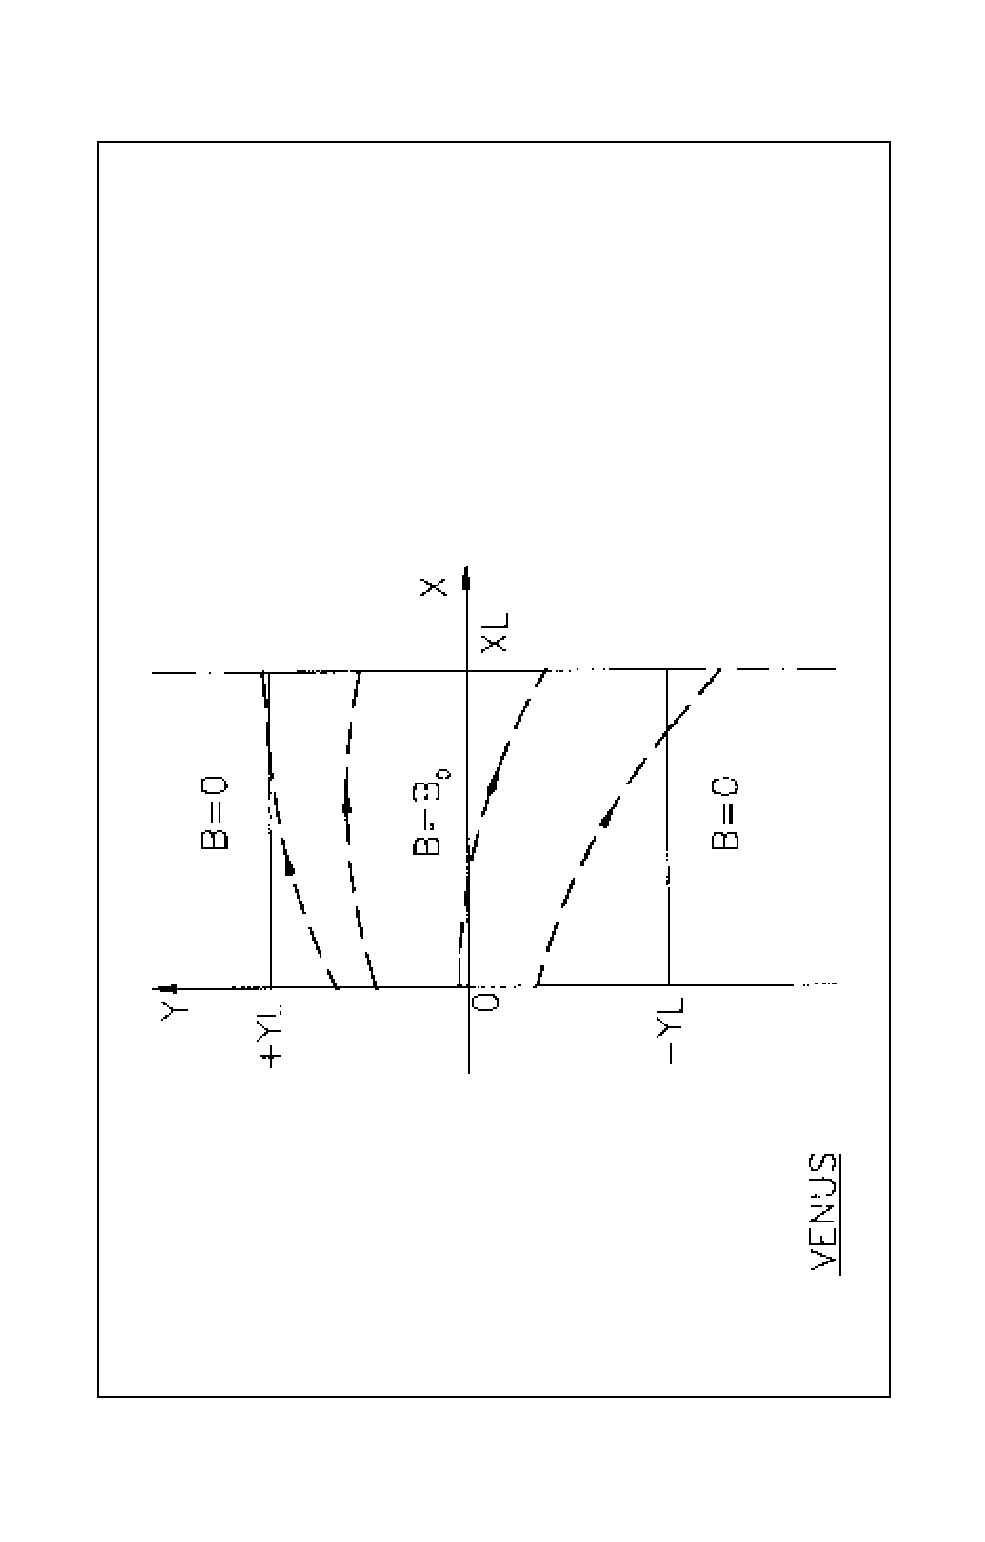
\includegraphics[height=15cm,angle=-90]{Fig32.ps}}
\unnumberedcaption{Scheme of \textsl{VENUS} rectangular dipole.}
\end{figure}
\vfill
\newpage

\begin{tabbing}
\mestab
 \textbf{WIENFILT~\footnotemark[1]}        \label{WIENFILT-B} \index{WIENFILT|textbf}
     \> \textbf{Wien filter} \> \> \\
 \\
 \\
 $\IL$   \>$\IL=1,2[\times 10^n],~7$ : print coordinates, fields, etc., along trajectories \>0-2$[\times 10^n]$, 7 \>I\\
        \> in zgoubi.res ($1$),  zgoubi.plt ($2$),  zgoubi.impdev.out ($7$).       \>                   \> \\
%  $\IL$            \>$\IL=1,2[\times 10^n]$ : print field and coordinates along trajectories.  \> 0-2$[\times 10^n]$\> I  \\
  \\
$ \XL$, $E$, $B$, $HV$      \>Length~; electric field~; magnetic field~; \> m, V/m, T, 
		\>3*E, I \\
\> option : element inactive ($HV=0$) horizontal \> 0-2 \> \\
      \> ($HV=1$) or vertical ($HV=2$) separation \\
\\
 \>\textbf{Entrance face :}  \> \> \\
 $X_{\text{E}}$, $ \lambda_{E_E}$, $ \lambda_{B_E}$       
        \>Integration zone extent~; fringe field \>  3*cm  \>3*E \\
 \>extents, E and B respectively ($\simeq$ gap height)  \> \> \\
  \\
$C_{E0}$--$C_{E5}$       \>Fringe field coefficients for $E$  \> 6*no dim.\>  6*E \\
$C_{B0}$--$C_{B5}$       \>Fringe field coefficients for $B$  \> 6*no dim.\>  6*E \\
 \\
 \>\textbf{Exit face :} \> \> \\
 $X_S$, $\lambda_{E_S} $, $ \lambda_{B_S}$      \>See entrance face \>  3*cm \> 3*E \\
 $C_{E0}$--$C_{E5}$       \>   \> 6*no dim.\>  6*E \\
$C_{B0}$--$C_{B5}$       \>   \> 6*no dim.\>  6*E \\
\\
 \textsl{XPAS}          \>Integration step  \>cm \>E \\
 \\
 \textsl{KPOS}, \textsl{XCE},    \textsl{YCE, ALE}     \>\textsl{KPOS}=1 : element aligned, 2 : misaligned~; shifts, tilt. 
           \>1-2, 2*cm, rad \>I, 3*E \\
\end{tabbing}
 
\footnotetext[1]{~ Use \textsl{PARTICUL} to declare mass and charge.}
 
  \newpage

\begin{tabbing}
\mestab
 \textbf{YMY}        \label{YMY-B} \index{YMY|textbf}
     \> \textbf{Reverse signs of $Y$ and $Z$ axes} \> \> \\
  \\
\\
 \> Equivalent to a 180$^\circ$ rotation with respect to $ X$-axis 
 \end{tabbing}
 \vfill
 
%%%%%%%%%%%%%%figure%%%%%%%%%%%%%%
\begin{figure}[H]
%\vspace{18 truecm}
%%%Figure 33
\centerline{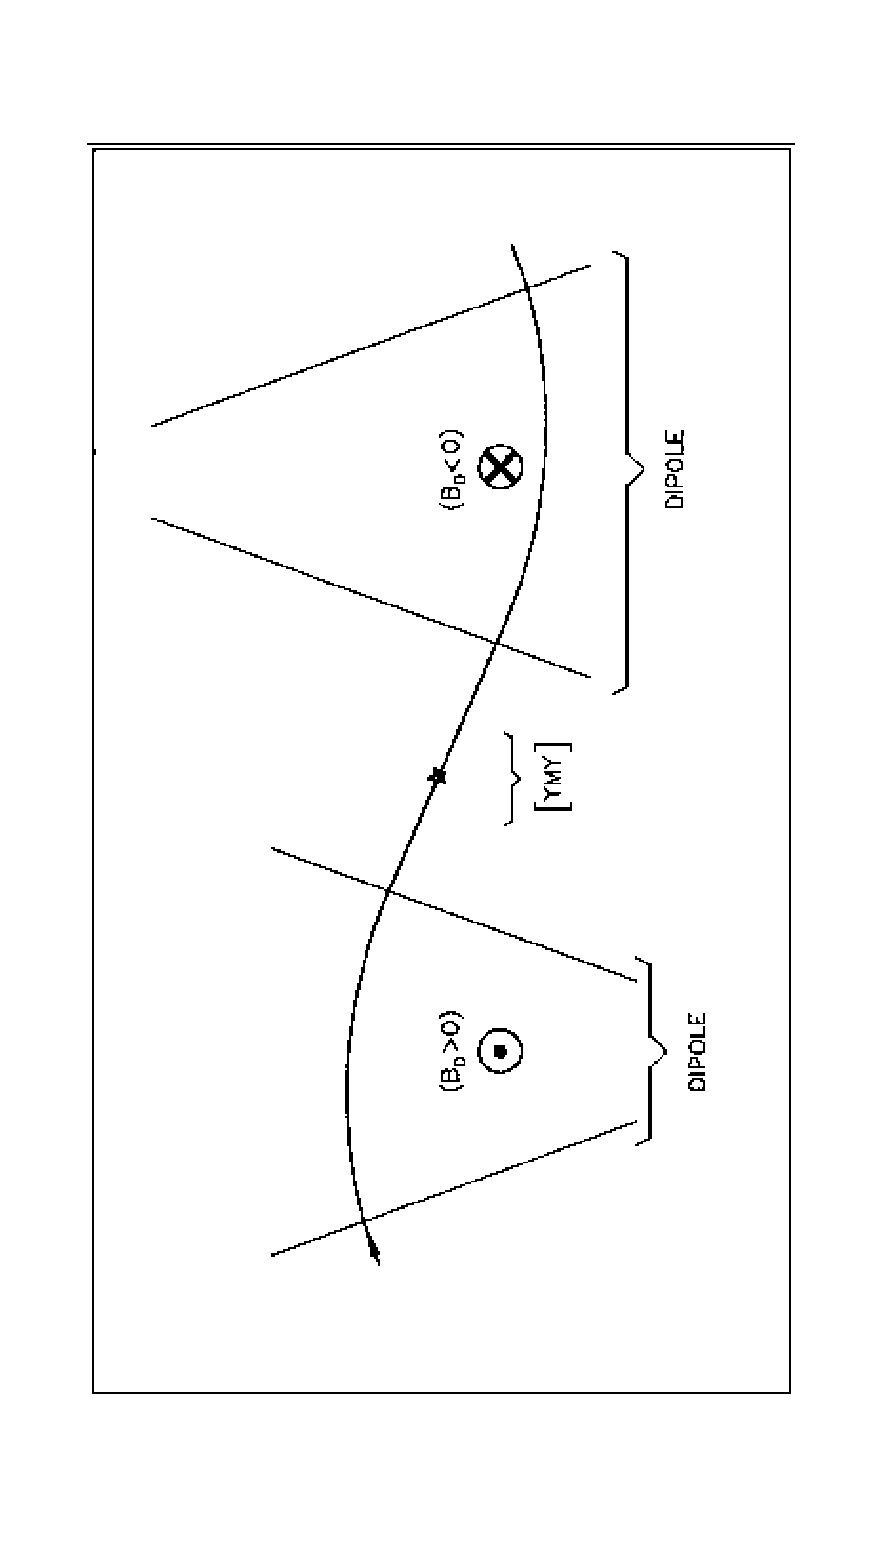
\includegraphics[height=15cm,angle=-90]{Fig33.ps}}
\unnumberedcaption{The use of $ YMY $ in a sequence of two 
dipoles of opposite signs.}
\end{figure}

\vfill
